\documentclass[a4paper]{article}

\usepackage[english]{babel}
\usepackage[utf8]{inputenc}
\usepackage{amsmath}
\usepackage{float}
\usepackage{graphicx}
\usepackage{subcaption}
\usepackage[colorinlistoftodos]{todonotes}
\usepackage{hyperref}
\usepackage[noabbrev,capitalise]{cleveref}
\usepackage{siunitx}
\usepackage{setspace}
\usepackage{soul}
\usepackage{multirow}
\usepackage[affil-it]{authblk}
\usepackage{verbatim}
\usepackage[bottom]{footmisc}
\usepackage[left=0.6in,right=0.6in,top=1in,bottom=1in]{geometry}
\usepackage[margin=0.6in]{caption}
\usepackage{multicol}
\usepackage{lineno}
\usepackage{array}
\usepackage{siunitx}
\usepackage{rotating}
\usepackage{makecell, tabularx}
\usepackage{soul}
\newcolumntype{C}{>{\centering\arraybackslash}X}
\linenumbers
\linespread{1.1}

\usepackage{listings}
\usepackage{xcolor}
\lstset { %
    language=C++,
    backgroundcolor=\color{black!5}, % set backgroundcolor
    basicstyle=\footnotesize,% basic font setting
}

\title{Measurement of $\nu_e$ interactions at low energy with the MicroBooNE Experiment}

\author[1]{Sophie Berkman}
\author[1]{David Caratelli}
\author[2]{Ivan Caro Terrazas}
\author[1]{Giuseppe Cerati}
\author[3]{Nicolo Foppiani}
\author[1]{Elena Gramellini}
\author[3]{Roxanne Guenette}
\author[2]{Ryan LaZur}
\author[2]{Michael Mooney}
\author[3]{Sebasten Prince}
\author[3,4]{Roberto Soleti}
\author[3,4]{Wouter Van De Ponteele}
\author[1]{Maya Wospakrik}
\affil[1]{Fermi National Accelerator Laboratory}
\affil[2]{Colorado State University}
\affil[3]{Harvard University}
\affil[4]{University of Oxford}
%\date{\today}	


\newcommand{\nue}{$\nu_e$ }
\newcommand{\nuecc}{$\nu_e CC$ }
\newcommand{\nueccnopinp}{$\nu_e CC 0\pi Np$ }
\newcommand{\nuebar}{$\bar{\nu}_e$ }
\newcommand{\nuebarcc}{$\bar{\nu}_e CC$ }
\newcommand{\numu}{$\nu_{\mu}$ }
\newcommand{\numucc}{$\nu_{\mu} CC$ }
\newcommand{\numubar}{$\bar{\nu}_{\mu}$ }
\newcommand{\numubarcc}{$\bar{\nu}_{\mu} CC$ }
\newcommand{\npsel}{1$e$N$p$0$\pi$ }
\newcommand{\zpsel}{1$e$0$p$0$\pi$ }

\begin{document}

\maketitle

\abstract{The analysis presented in this note uses data from the MicroBooNE Experiment to measure  $\nu_e$ interactions from the Booster Neutrino Beamline using the Pandora reconstruction framework. Our goal is addressing the nature of the anomalous excess of low-energy events with EM activity in the final state as recorded by the MiniBooNE experiment. In this document, we outline the analysis strategy, focusing on the reconstruction and event selections performed, the evaluation of systematics associated to detector, flux, and neutrino-interaction modeling, and the expected sensitivity to the MB-$\nu_e$ LEE model utilizing the available BNB dataset of 10.1$\times 10^{20}$ POT. }

\tableofcontents

\newpage
\section{Technical Overview on the Content of this Note \textcolor{red}{David+Elena}}
Before we dive into the physics, we take a moment to lay out some technical details, common conventions, and acronyms used throughout this note. This is intended to help the reader through the note's interpretation.
%\addcontentsline{toc}{Section}{echnical Overview on the Content of this Note}
\subsection{Samples}
\par This analysis attempts to use all the latest available data and simulation samples for the MicroBooNE LEE analysis. This section briefly describes which samples are used.
\par MicroBooNE's collected dataset passing  data-quality requirements for the LEE analysis consists of 10.1E20 POT of BNB data taken over four ``runs'', or data taking periods. %This number takes into account run periods discarded due to data-quality requirements. 
Only small subsets of this data is available for analyzers to use, i.e. :
\begin{itemize}
\item[-] On-beam data (\textbf{BNB}):
\begin{itemize}
\item ``5E19'' POT Run1 open dataset (4.07E19 POT after quality cuts)
\item  ``1E19'' POT Run3 open dataset  (0.8E19 POT after quality cuts) 
\item  $\sim3.0$E20 POT of filtered $\pi^0$ data from Runs 1 and 3. 
\end{itemize}
\item[-] Off-beam data (\textbf{EXT}):
\begin{itemize}
\item all available Run1 samples (about 1 million events)
\item all available Run3 samples (about 1 million events)
\end{itemize}
\item[-] MC (from the ``overlay datasets''):
\begin{itemize}
\item $\sim$1E21 POT standard MC BNB flux prediction
\item $\sim$5E22 POT $\nu_e$ intrinsic only from the standard MicroBooNE flux prediction
\item $\sim$3E20 POT  \emph{dirt} interactions (neutrinos which interact outside of the cryostat) 
\item $\sim$2-3E21 POT filtered by final-state topology for CC $\pi^0$ and NC $\pi^0$ events
\end{itemize}
\end{itemize}

%For on-beam data, three samples are used in this note: the ``5E19'' Run1 open dataset ($4.07E19$ POT after quality cuts), the ``1E19'' ($0.8E19$ POT after quality cuts) open Run3 data, and the $\sim3.0E20$ POT of filtered $\pi^0$ data from runs 1 and 3. 
%For off-beam data, this analysis uses all available samples from Run1 and Run3, consisting of roughly 1 million events for each run. 

Scaling factors for the EXT datasets to match the full 10.1E20 POT are $\times3.5$ and $\times2.1$ for Run1 and Run3 respectively. The fact that EXT samples need to be scaled up rather then down is a consequence of the lack of availability of off-beam events. This is a generally recognized problem with all LEE analyses and may make EXT background estimation difficult and hamper sensitivity estimates.
\par %All MC samples used are from ``overlay datasets''. For each run period, MC datasets are produced for the standard MC BNB flux prediction (``MC'' sample, $\sim1E21$ POT), a $\nu_e$ intrinsic sample simulating only $\nu_e$ neutrinos from the standard MicroBooNE flux prediction (\emph{$\nu_e$ intrinsic}, $\sim5E22$ POT), a sample of \emph{dirt} interactions (neutrinos which interact outside of the cryostat, $\sim3E20$ POT), and samples filtered by final-state topology for CC $\pi^0$ and NC $\pi^0$ channels ($\sim2-3E21$ POT). 
All simulation samples, in addition to the generic ``MC'' are used to boost statistics in channels that are sub-dominant in event rate but important for this analysis. In merging these samples in the analysis, we take care to remove the same events from the ``MC'' samples and weigh the special high-statistic samples appropriately. 
Even with this workflow, the statistics of several background categories are not sufficient for a careful evaluation of their impact on the selection. This leads to large bin-by-bin fluctuations in the expected events and therefore an unclear background estimation. To mitigate this, specific targeted truth-based filters have been developed (see DocDB 27409~\cite{bib:truthfilters}) to boost statistics in backgrounds for which the current statistics are not sufficient. 

\subsection{How to read plots in this note} A large fraction of plots in this note are data-simulation comparisons. This paragraph describes common features for these plots. All data-simulation comparisons up to Chapter~\ref{sec:systematics} show statistical errors only, denoted with error-bars for data. The statistical error on MC samples is denoted with a grey band. All plots, unless otherwise labeled, are POT normalized, following the procedure outlined in DocDB 15204~\cite{bib:POTscaling}. Data-simulation comparisons are accompanied by a legend which denotes the various event categories shown. Categories are described below:
\begin{itemize}
    \item \textbf{BNB}: On-beam contributions (data).
    \item \textbf{EXT}: Off-beam contributions (data).
    \item \textbf{Cosmic}: Events from MC overlay where a cosmic instead of a neutrino interaction have been selected as the neutrino candidate by Pandora's \texttt{SliceID}.
    \item \textbf{Out. fid. vol.}: Events from MC overlay where a neutrino was tagged, but the neutrino interaction vertex is outside of the defined TPC fiducial volume.
    \item \textbf{MiniBooNE LEE}: Events from the MB-$\nu_e$ LEE model.
    \item \textbf{$\nu_e$}: CC $\nu_e$ events, split by final state (\zpsel, \npsel, and N$\pi$).
    \item \textbf{$\nu_{\mu}$ CC}: CC muon events with no final state $\pi^0$.
    \item \textbf{$\pi^0$}: $\nu_{\mu}$ events with final state $\pi^0$ split in NC and CC channels.
    \item \textbf{NC}: NC events (all flavors) with no final state $\pi^0$s.
\end{itemize}{}

\subsection{Tech-note versioning: current status and recent/expected changes }
Until Neutrino2020, this note is supposed to be a living document: this entails that parts of the analysis will evolve and parts of the text is going to change. Throughout the note, we highlight incomplete parts and known preliminary statements with the use of \emph{italics}.

\par As of January 2020,  all latest samples are used, including the ``GENIE-TUNE CV" weights for work up to the selections development.
For systematic studies, the latest GENIE and flux systematics are used to present truth-level studies, but they are not used for the final sensitivity calculation due to ongoing work in SBNFit to incorporate them.
%\begin{multicols}{1}

\newpage

\section{Introduction to the $\nu_e$ analysis}
In this section, we provide the big picture view of the complete Pandora $\nu_e$ analysis, starting from our selection philosophy and ending with our strategy regarding systematics. A deeper dive into on each topic is provided in note's following sections. 

\subsection{$\nu_e$ Selection Philosophy \textcolor{green}{David ... (P.R. Elena) }}
\par Several proposals have been made to explain the nature of the MiniBooNE LEE anomaly. It is fair to say that a large amount of uncertainty remains in the community regarding what may have generated such an excess of EM events: this analysis works within the $\nu_e$ excess hypothesis.  To best explore the potential new physics in the $\nu_e$ channel at low energy, this analysis aims to perform an inclusive multi-channel measurement of $\nu_e$ interactions without relying on kinematic variables which depend upon neutrino-interaction models. A multi-channel approach can reduce systematic uncertainties dependent on the chosen interaction model in addition to building a stronger confidence against  issues in the MC simulation.

\par By performing three different $\nu_e$ selections, we aim at isolating three channel topologies: the $\nu_e$ inclusive, 1$e$N$p$0$\pi$, and a 1$e$0$p$0$\pi$ channels. A schematic summarizing the strengths and features of each selection is shown in table~\ref{tab:selectionsNue}. The 1$e$N$p$0$\pi$ and 1$e$0$p$0$\pi$ selections are orthogonal and share a common pre-selection, which splits at the stage in which presence of a final state proton in the event is determined; these two channels combined match the MiniBooNE signal channel (1$e$X$p$0$\pi$). The inclusive $\nu_e$ selection currently is developed independently of the other two selections: therefore, its selected events are not orthogonal to the 1$e$X$p$0$\pi$ pool of candidates.
%\textcolor{red}{Should we add that our main selection is the 1$e$N$p$0$\pi$? }

\begin{comment}
\par We perform three $\nu_e$ selections, each aimed at leveraging particular strengths, and designed with cuts tailored to exploit as much information in a given channel topology as possible. The analysis is comprised of a $\nu_e$ inclusive, a 1$e$N$p$0$\pi$, and a 1$e$0$p$0$\pi$ selection. A schematic summarizing the strengths and features of each selection is shown in table~\ref{tab:selectionsNue}. The 1$e$N$p$0$\pi$ and 1$e$0$p$0$\pi$ selections are orthogonal and share a common pre-selection, which splits at the stage in which presence of a final state proton in the event is determined; these two channels combined match the MiniBooNE signal channel (1$e$X$p$0$\pi$). The inclusive $\nu_e$ selection currently is developed independently of the 1$e$N$p$ selection and therefore its selected events are not independent.
\end{comment}



%\begin{figure}[ht]
%\begin{center}
%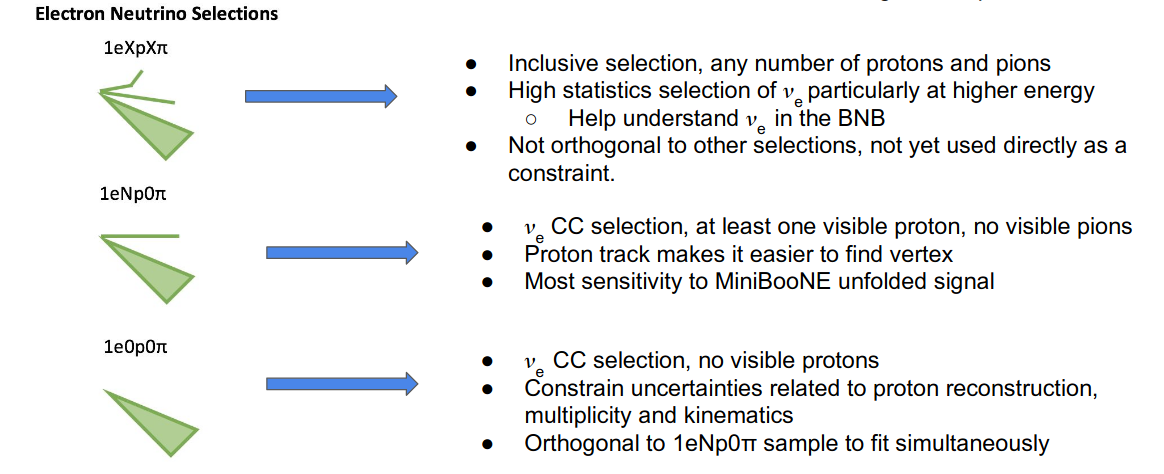
\includegraphics[width=0.85\textwidth]{introduction/nueselections.png}
%\caption{\label{fig:nueselections}Schematic of the three $\nu_e$ selection in this analysis, outlining the goals and strengths of each. In this work, the threshold for a visible proton at truth-level proton is 40 MeV of KE. $N$ refers to one or more and $X$ to any number of final state particles of a given category.}
%\end{center}
%\end{figure}


\begin{table}[ht]
\caption{\label{tab:selectionsNue} Schematic of the three $\nu_e$ selections, outlining the definition and goals of each. In this work, the threshold for a visible proton at truth-level proton is 40 MeV of KE. N refers to one or more and X to any number of final state particles of a given category.}
\centering
\begin{tabular}{ m{0.1\textwidth} | m{0.2\textwidth}  m{0.45\textwidth}  }
Channel & Description & Goal \\
\hline
 \begin{center}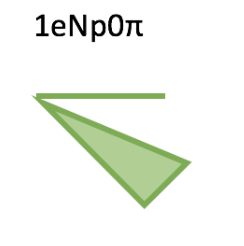
\includegraphics[width=0.1\textwidth]{introduction/1eNp}\end{center}& At least one visible proton and no visible pions & Most sensitive channel to MiniBooNE unfolded signal. The presence of a proton facilitates vertex finding.\\
\hline
 \begin{center}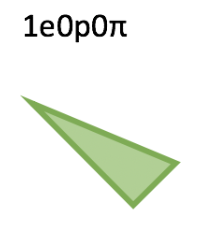
\includegraphics[width=0.1\textwidth]{introduction/1e0p}\end{center}& No visible protons and no visible pions & Constrain uncertainty related to proton reconstruction, multiplicity and kinematics for the 1$e$N$p$0$\pi$ channel.\\
\hline
\begin{center}\includegraphics[width=0.1\textwidth]{introduction/inclusive} \end{center} & Inclusive Selection: any number of protons and pions & Helpful to understand $\nu_e$ in the BNB: high statistic selection, especially at higher energies ($>$ 700 MeV). Not used as a constraint for other channels. \\
\hline
\end{tabular}
\label{tab:gt}
\end{table}


\par %\textbf{agnostic selection} 
In devising the selections presented above, we have deliberately chosen to not rely on cuts that make use of kinematic features of low-energy $\nu_e$ events. This allows the analysis to be agnostic to possible sources of new physics, and limits model dependence associated with assumptions on intrinsic $\nu_e$ interaction kinematics. Furthermore, an agnostic selection strategy allows to explore the kinematics of $\nu_e$ candidate events after their selection, for a full investigation of the origin of a potential anomaly. Implementing this choice requires the ability to fully leverage the information provided by the MicroBooNE LArTPC for $\nu_{\mu}-\nu_e$ and $e-\gamma$ separation. Significant progress has been made in developing tools for this goal, and will be described in subsequent sections. 




\subsection{Signal Model \textcolor{green}{David  ... (P.R. Elena) }}
\begin{comment}
%%%%%%% these are various parts that have been moved/modified
In order to benchmark the performance of the analysis it is valuable to have a signal model which can be used to assess the analysis' sensitivity.  This section describes the choice of model used for this purpose. It is important to stress that the signal model used serves the purpose of benchmarking the analysis' sensitivity, but the ultimate goal of our analysis remains to measure the rate of $\nu_e$ interactions in the BNB and report whether the observation is consistent or not with MicroBooNE's MC prediction.

\par Ultimately many signal models can be produced to test an analysis' sensitivity, each with its own set of important assumptions and caveats. % Or...
Ultimately any signal model used to test the analysis' sensitivity will carry a set of important assumptions and caveats. 
While reporting sensitivities for the MB-$\nu_e$ LEE model is useful, it is not exhaustive in being able to address MicroBooNE's ability to address MiniBooNE's anomaly. 
\end{comment}


\par  Many models can be devised to explain the MiniBooNE LEE as an excess of $\nu_e$ interactions, each model relying on a given (new) physics production mechanism and set of assumptions on the detector response. This section describes the signal model chosen by the collaboration to benchmark the sensitivity of all $\nu_e$ LEE analyses, including ours.  While a signal model is a useful tool, it is important to stress that any signal model carries a set of important assumptions and caveats, and that the ultimate goal of our analysis remains to measure the rate of $\nu_e$ interactions in the BNB, reporting whether the observation is consistent or not with MicroBooNE's MC prediction. Answering whether MicroBooNE's observation is consistent with the MiniBooNE LEE anomaly is beyond the scope of this work, and something not achievable without significant work for both MiniBooNE and MicroBooNE.
\begin{comment}
\par To test this analysis' sensitivity, a model explaining the MiniBooNE LEE  as an excess of $\nu_e$ interactions must be produced and used to generate simulated events in MicroBooNE. Many such models can be devised, each relying on a given (new) physics production mechanism and set of assumptions on detector response. 
\end{comment}

\par  The signal model used to generate simulated events in MicroBooNE and to compute the primary sensitivity quoted by this analysis  is the MiniBooNE-unfolded LEE model, referred to as \textbf{MB-$\nu_e$ LEE} model \cite{C,C2}. In this model, all excess LEE events are assumed to be due to $\nu_e$ interactions with a value of true energy obtained by unfolding from the reconstructed CCQE energy of MiniBooNE LEE events, as recorded by MiniBooNE's data. This procedure is performed by relying on MiniBooNE's energy smearing matrix. The resulting true neutrino energy distribution is shown in figure~\ref{fig:minibooneunfolded}. There are several limitations to this model worth observing, some technical, others conceptual. On a technical level, the model is composed of a binned event distribution, rather then a parametrized or analytic prediction of the expected $\nu_e$ spectrum. Additionally, no events below 200 MeV of true energy exist in this model. 
\begin{figure}[ht]
\begin{center}
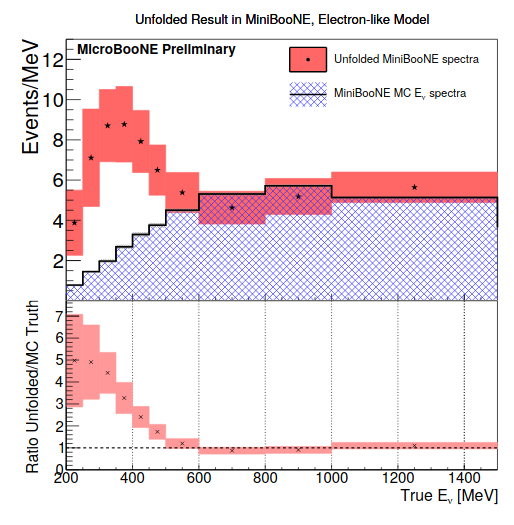
\includegraphics[width=0.45\textwidth]{introduction/unfoldedminiboone.png}
\caption{\label{fig:minibooneunfolded}MB-$\nu_e$ LEE signal model extracted from MiniBooNE's results.}
\end{center}
\end{figure}
Conceptual issues can be raised in association with the various assumptions made to generate the model. These include the strong reliance on MiniBooNE's simulation in order to unfold reconstructed to true neutrino energy, and the choice of such an unfolding procedure (performed as a function of $E_{\rm CCQE}$ rather then EM energy and $\theta$, for example).
It is especially important to note that the chosen model strongly favors the interpretation of MiniBooNE events as originating from very low energies (200-400 MeV) for which achieving high sensitivity may come at the cost of omitting a robust analysis at higher energies. This is something the analysis tries to avoid by developing an inclusive and kinematically unbiased analysis workflow. At the same time, we explore additional models for sensitivity calculations, most notably a 3+1 sterile-neutrino oscillation model. This is discussed in more detail in section~\ref{sec:Sensitivity2Osc}.
\par Figure~\ref{fig:nuerate} shows the expected $\nu_e$ rate as a function of true neutrino energy split by final-state topology for the available MicroBooNE dataset of $10.1E20$ POT. % with a 10 cm FV. 
 MB-$\nu_e$ LEE signal events are shown in orange.
\begin{figure}[H] 
\begin{center}
    \begin{subfigure}[b]{0.45\textwidth}
    \centering
    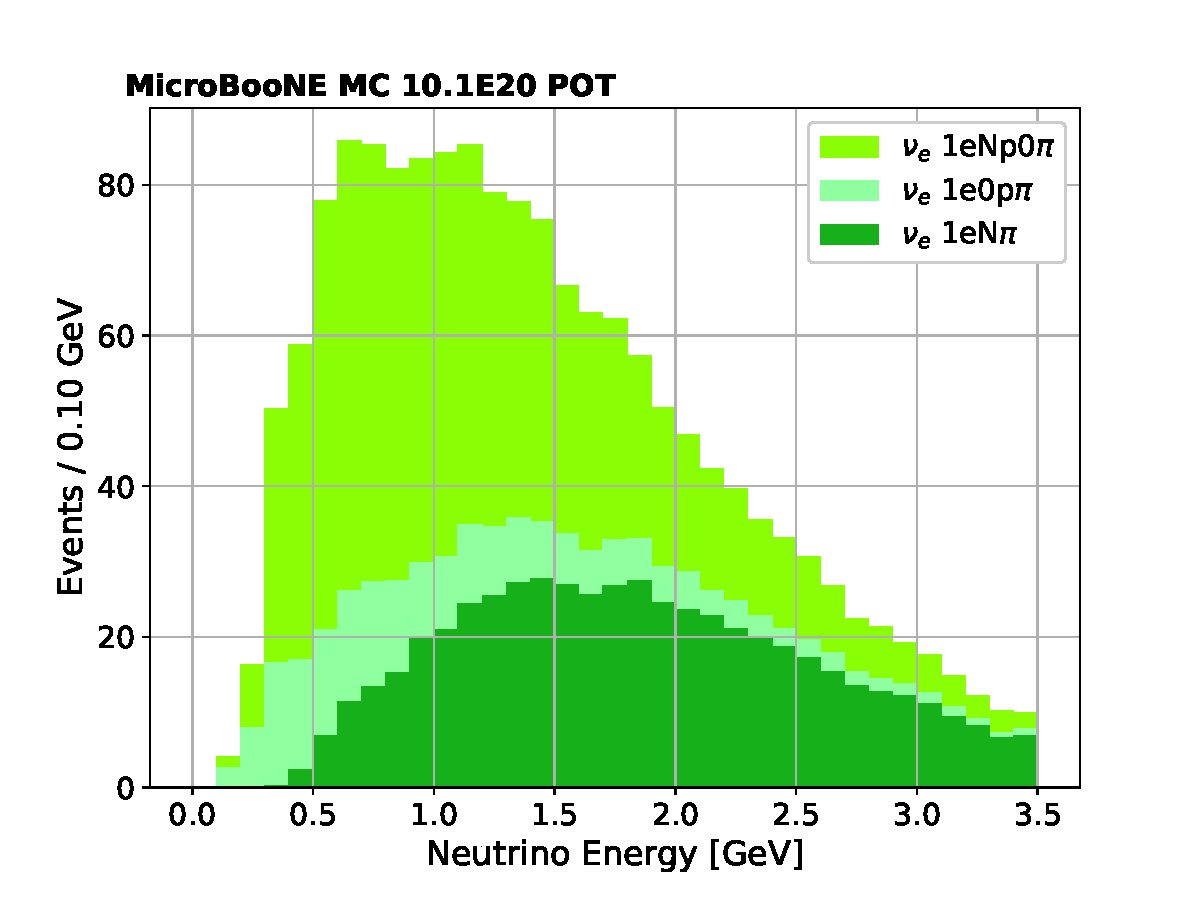
\includegraphics[width=1.00\textwidth]{introduction/nue_rate_MCC9.pdf}
    %\caption{\label{fig:nuerate:prediction}}
    \end{subfigure}
    \begin{subfigure}[b]{0.45\textwidth}
    \centering
    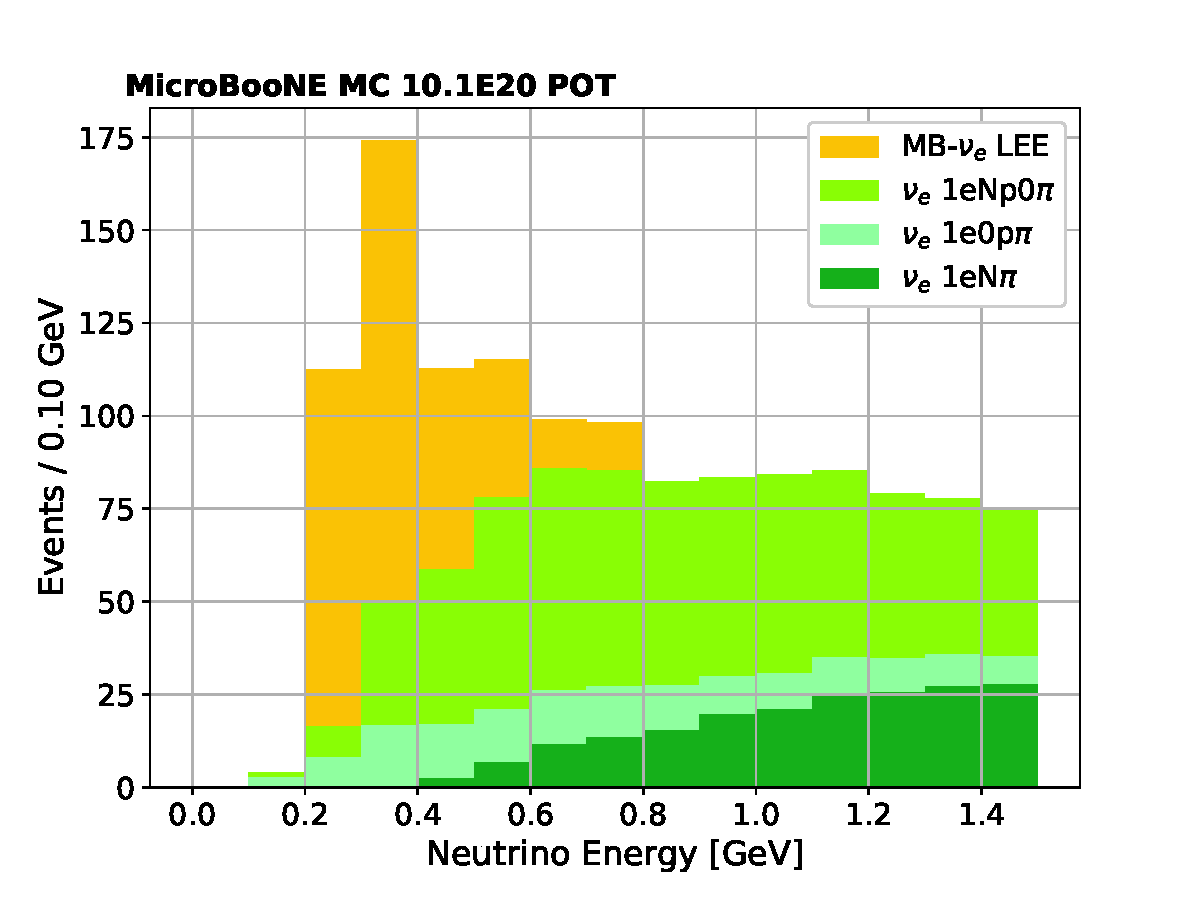
\includegraphics[width=1.00\textwidth]{introduction/nue_rate_MCC9_LEE.pdf}
    %\caption{\label{fig:nuerate:prediction:MC}}
    \end{subfigure}
\caption{\label{fig:nuerate}Expected $\nu_e$ rate in MicroBooNE for $10.1E20$ POT %in a 10-cm FV 
 subdivided by event topology (1$e$N$\pi$,1$e$N$p$0$\pi$, and 1$e$N$p$0$\pi$). The right-hand side figure highlights the low energy region with the unfolded $MB-\nu_e$ LEE signal prediction in orange.}
\end{center}
\end{figure}

\subsection{Goals of the $\nu_{\mu}$ Selection \textcolor{green}{David   ... (P.R. Elena)}}
\label{ssec:goalsofnumusel}
\begin{comment}
\par For the purpose of this analysis, measurements of $\nu_{\mu}$ interactions are aimed at reducing modeling uncertainties for intrinsic $\nu_e$ events and backgrounds, with the goal of reducing systematic uncertainties in order to be able to claim the observation of new physics were a measurement of $\nu_e$ interactions differ significantly from the expected intrinsic rate. This section describes why such a data-driven constraint is needed and what are the choices which motivate the approach taken in this analysis.
\end{comment}
\par In the context of this analysis, measurements of $\nu_{\mu}$ interactions are aimed at reducing modeling uncertainties for intrinsic $\nu_e$ events and backgrounds. Event reconstruction and $\nu_e$ identification are only one of the challenges in this analysis:  in order to make statements on whether the observed $\nu_e$ rate indicates the presence of new physics, a well understood prediction of the intrinsic $\nu_e$ rate is needed. 

\par Uncertainties in the expected $\nu_e$ rate are associated to reconstruction efficiencies (detector effects) as well as modeling uncertainties in both the $\nu_e$ flux  and neutrino-argon cross-section predictions. Here, we focus on describing the strategy to deal with the latter. In the case of a single detector experiment, %uncertainties in the intrinsic $\nu_e$ interaction rate are rather large:  and can limit the ability to associate a $\nu_e$ measurement with potential new physics if not a constraint through additional measurements is needed. 
flux uncertainties for $\nu_e$ calculated from the beam simulation are $\mathcal{O}$(10\%) above 800 MeV and grow to 40\% at 200 MeV;  cross-section uncertainties are also large, due to the scarcity of $\nu$-Ar cross-sections measurements -- especially at low energy -- and due to the complex modeling of neutrino interactions on heavy targets such as argon. Combining all effects, the uncertainty on the $\nu_e$ interaction rate in the few-hundred MeV energy range in MicroBooNE could be as high as 100\%.
\par To reduce modeling uncertainties on the expected rate of $\nu_e$ interactions, data-driven constraints are required. These can be performed through measurements of $\nu_{\mu}$ interactions impacted by the same underlying modeling uncertainties. In order to constrain flux uncertainties, we rely on the fact that $\nu_e$ and $\nu_{\mu}$ intrinsic to the beam are produced by the decay of the same parent $\pi$ and $K$ flux. Similarly, we rely on the charged-current interaction mode $\nu_{l} + Ar \rightarrow l + X$ common to both $\nu_{\mu}$ and $\nu_e$ interactions to constrain the uncertainties on the $\nu_e$ interaction modeling.


\begin{comment}

The complexity of $\nu$-Ar interactions and of hadronic interactions in the beamline mean that many different handles and measurements of $\nu_{\mu}$ interactions can play a role in constraining different uncertainties. As examples, measurement of CC and NC $\pi^0$ production constrain resonant interactions and thus $\pi^0$ backgrounds to the $\nu_e$ selection, and measurements of high-energy $\nu_{\mu}$ interactions can help constrain the kaon flux in the beam, which contributes substantially to the production of intrinsic $\nu_e$s. Likewise, measurements of low-energy $\nu_{\mu}$s can help constrain poorly understood $\nu$-Ar interaction models in the few-hundred MeV energy regime, a critical requirement for this analysis. The neutrino identification work developed for this analysis, referred to as \texttt{SliceID} and described in section~\ref{sec:sliceID}, is a highly efficient and topology agnostic selection that enables a vast program of $\nu_{\mu}$ measurements, allowing for flexibility in selecting topologies that may have the strongest constraining power and thus most benefit the $\nu_e$ analysis. At the current time, as described in the remainder of this section and in section~\ref{sec:systematics}, the emphasis is on the measurement of low-energy $\nu_{\mu}$ interactions with the goal of constraining the large uncertainties in low-energy $\nu_e$ events which significantly impact the analysis.
\par To further motivate the need for low energy $\nu_{\mu}$ interactions, we describe two important ways in which such a dataset can benefit the reduction of modeling uncertainties for $\nu_e$ interactions.
\end{comment}
\par The richness of $\nu$-Ar interactions and of hadronic interactions in the beamline offers a number of different handles 
to constraint different uncertainties via the measurements of $\nu_{\mu}$ interactions.
As examples, measurements of CC and NC $\pi^0$ production can be used to constrain resonant interactions and thus $\pi^0$ backgrounds to the $\nu_e$ selection;  measurements of high-energy $\nu_{\mu}$ interactions can help constrain the kaon flux in the beam, which contributes substantially to the production of intrinsic $\nu_e$s. Likewise, measurements of low-energy $\nu_{\mu}$s can help constrain poorly understood $\nu$-Ar interaction models in the few-hundred MeV energy regime, a critical requirement for this analysis.  At the current time, we focus our effort on the study with the bigger impact to the analysis: we perform the measurement of low-energy $\nu_{\mu}$ interactions with the goal of constraining the large uncertainties in low-energy $\nu_e$. A detailed  description of this constraint is shown in the remainder of this section and in section~\ref{sec:systematics}.
%At the current time, our effort is focused on the measurement of low-energy $\nu_{\mu}$ interactions with the goal of constraining the large uncertainties in low-energy $\nu_e$ events which significantly impact the analysis; a detailed  description of this constraint is shown in the remainder of this section and in section~\ref{sec:systematics}.
 However, it should be noted that the neutrino identification work described in section~\ref{sec:sliceID} results in a highly efficient and topology agnostic selection: such a flexible selection allows for a number of $\nu_{\mu}$ measurements and their associated constraints to be implemented in case the $\nu_e$ analysis needs a stronger constraining power. 



\par To further motivate the need to study low energy $\nu_{\mu}$ interactions, we describe two important ways in which such a dataset can lead to a reduction of modeling uncertainties for $\nu_e$ interactions. Figure~\ref{fig:numuconstraint:flux} shows the flux correlation for $\nu_{\mu}$ (bottom left) and $\nu_e$ (top right) interactions obtained from MicroBooNE's adaptation of the BNB flux simulation developed by MiniBooNE~\cite{bib:fluxmcc9,bib:fluxtechnote}. Red (blue) areas show large (anti-)correlation. The top-left or bottom-right quadrants show the strength of correlations between the two flavors. For $\nu_e$ energies below 1 GeV, correlations are strongest with $\nu_{\mu}$ interactions at low energy \textcolor{blue}{should we add some more details on the assumptions behind this correlation matrix? or on how this correlation matrix is calculated (is it simply from the beam MC?) Elena}. Figure~\ref{fig:numuconstraint:xsec} shows different cross-section predictions for $\nu_{\mu}$ and $\nu_e$ interactions. The dashed and solid curves represent the CCQE cross-section used in MCC8 vs. MCC9 respectively. Below 400 MeV, the difference in event rates for different models is larger then 100\%. The large differences between these curves, particularly at low energy, indicate the strong need to constrain cross-section uncertainties with MicroBooNE's own data. 
\begin{figure}[ht] 
\begin{center}
    \begin{subfigure}[b]{0.42\textwidth}
    \centering
    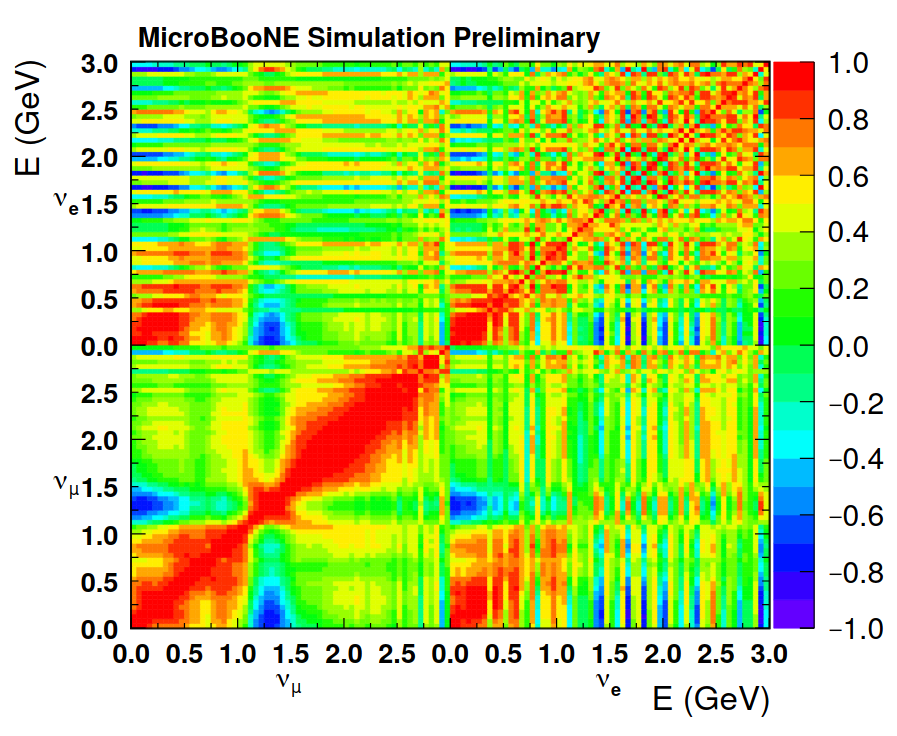
\includegraphics[width=1.00\textwidth]{introduction/fluxcorrelation.png}
    \caption{\label{fig:numuconstraint:flux}}
    \end{subfigure}
    \begin{subfigure}[b]{0.3\textwidth}
    \centering
    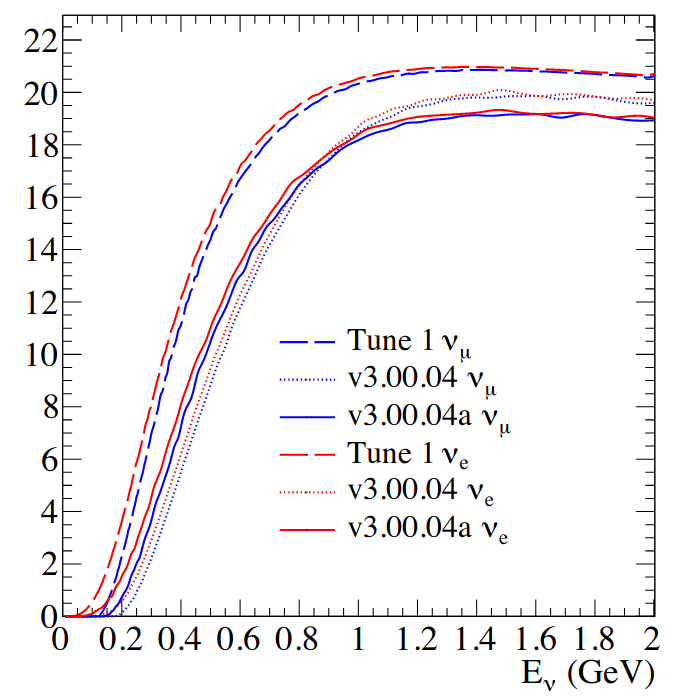
\includegraphics[width=1.00\textwidth]{introduction/xsec_mcc8_mcc9.png}
    \caption{\label{fig:numuconstraint:xsec}}
    \end{subfigure}
\caption{\label{fig:numuconstraint} (a) $\nu_{\mu}$-$\nu_e$flux correlation matrix. (b) Different cross section models for CC interactions \textcolor{blue}{Y axis label is missing}.  }
\end{center}
\end{figure}

\subsection{Systematics \textcolor{green}{David... (P.R. Elena)}}
\par This section gives a brief overview of how detector and modeling uncertainties are accounted for in the analysis. The estimation of systematics is performed in section~\ref{sec:systematics}.
\par \noindent \textbf{Detector Systematics}: Detector modeling in MicroBooNE has undergone significant updates in the past year, in part as a result of the large impact that detector systematics have had on 2018 analyses \cite{bib:CCpi0, bib:CCincl}. Detector effects with significant impact on the analysis can be broken up into three main categories:
\begin{itemize}
    \item[-] Wire-Response modeling: the response of MicroBooNE's electronics to drifting charge is a complex subject described in three past publications~\cite{bib:noise,bib:SP1,bib:SP2}. The work of these papers in improving the understanding and modeling of noise and field-response effects has been implemented in the current detector simulation and is expected to lead to a reduction in what for MCC8 analysis comprised the largest detector uncertainty.
    \item[-] Space-Charge modeling: MicroBooNE's space-charge model has changed significantly since 2018, moving from a calculation-based~\cite{bib:SCEsim} implementation of electric field distortions to a data-driven E-field map~\cite{bib:SCEdata} implemented in simulation and reconstruction. Due to the large position distortions (and, though smaller, charge distortions) SCE can significantly impact an analysis through the determination  of fiducial boundaries, tracking and energy resolution.
    \item[-] Scintillation light modeling: MicroBooNE's model of scintillation light production has not changed significantly since the beginning of data-taking, and has known limitations. Of particular importance to this analysis, which aims to use a dataset spanning four years, is the known and significant time-dependent variation of MicroBooNE's light response. This analysis takes several steps to correct for, and mitigate the impact of light mismodeling. Triggering on low-energy signal $\nu_e$ events, and cosmic-rejection are particularly sensitive to scintillation light detector effects.
\end{itemize}
\emph{An additional detector effects that needs to be accounted for is ion Recombination which impacts the detector's calorimetric response. Tailored studies and proton samples are being developed to assess ion recombination modeling accuracy in MCC9 but are not available at the time of writing of this note.}
\par \noindent \textbf{Flux and Cross-Section Modeling} Uncertainties in flux and cross-section modeling are treated through a \emph{multi-sim} approach, where underlying parameters that are input to the modeling are varied in a correlated way. Flux uncertainties are taken from the MiniBooNE BNB flux simulation adapted to MicroBooNE~\cite{bib:fluxmcc9,bib:fluxtechnote}, while $\nu$ interaction uncertainties are handled within the \texttt{GENIE} reweighting package, as described in~\cite{bib:geniesupportnote}. \emph{We note that the \texttt{GENIE} event reweighting infrastructure is still in development and likely to be updated or further expanded on in the future. Finally, uncertainties associated with pion and proton re-interactions in argon were unavailable when this version of the Tech Note was produced and not included at this stage.} 

\subsection{Sensitivity Estimation \textcolor{green}{Nico/Maya... (P.R Elena)}}
In order to extract information from the selected events, a simple hypothesis test is performed.
Given an observable quantity, such as a measurement of the energy deposited by the neutrino interaction, the hypothesis in which the observed spectrum of events is entirely due to the standard model, $H_0$, is tested against an alternative hypothesis $H_1$.
The alternative hypothesis $H_1$ consists of all the known background plus the LEE unfolded signal from MiniBooNE (MB-$\nu_e$ LEE), though an oscillation signal has also been studied, as shown in section \ref{sec:Sensitivity2Osc}.
For the MB-$\nu_e$ LEE signal, the hypothesis test is simple in that the comparison of two different hypotheses is performed and no parameter is inferred from the data.

%The hypothesis test is simple in the sense no parameter is fitted from the data, but we limit ourselves to a comparison of two different hypotheses.

A test statistic is chosen in order to condensate all information of the observables in one number.
Through toy experiments, the expected distributions of the test statistic under the two hypotheses is calculated; the separation power is computed by taking the median p-value with respect to $H_0$ under the assumption that %one might observe if 
 $H_1$ is true. This is the discovery sensitivity, i.e. the sensitivity to reject $H_0$ when $H_1$ is true.
We studied the sensitivity in different cases. First, we describe in detail the sensitivity calculation considering only statistical uncertainties. Given that only a handful of events pass the exclusive selections, the impact of statistical uncertainties plays a large role in determining the analysis' ultimate sensitivity. We also include systematic uncertainties using the covariance matrix formalism and the SBNfit package, as described in section \ref{subsec:sensitivity_syst_uncertainty}.
Finally, the observed spectra from the \nueccnopinp and the \numu selections are analyzed simultaneously using a single covariance matrix to constraint the systematic uncertainties and thus increase the sensitivity.

\subsection{Analysis Status \textcolor{red}{Elena/David/ Group discussion}}

\par The work presented in this note has matured into a robust and comprehensive analysis, with strong tools which are able to leverage the calorimetric and topological imaging of the LArTPC technology to identify in a kinematically agnostic selection $\nu_e$ interactions in MicroBooNE's BNB dataset. The analysis, as it stands, is able to make interesting conclusions on the $\nu_e$ content of the BNB flux, with the primary limitation to the power of these conclusions driven by the low selection efficiency at low energy .
\par Multiple selections have been developed as part of this analysis, all showing generally good data-simulation agreement, as shown in figure~\ref{fig:datamccomparisons} for the \npsel pre-selection (figure~\ref{fig:datamccomparisons:nuepresel}, Run 1) and for the full $\nu_{\mu}$ contained selection (figure~\ref{fig:datamccomparisons:numu}, Run 3).

\begin{figure}[ht] 
\begin{center}
    \begin{subfigure}[b]{0.4\textwidth}
    \centering
    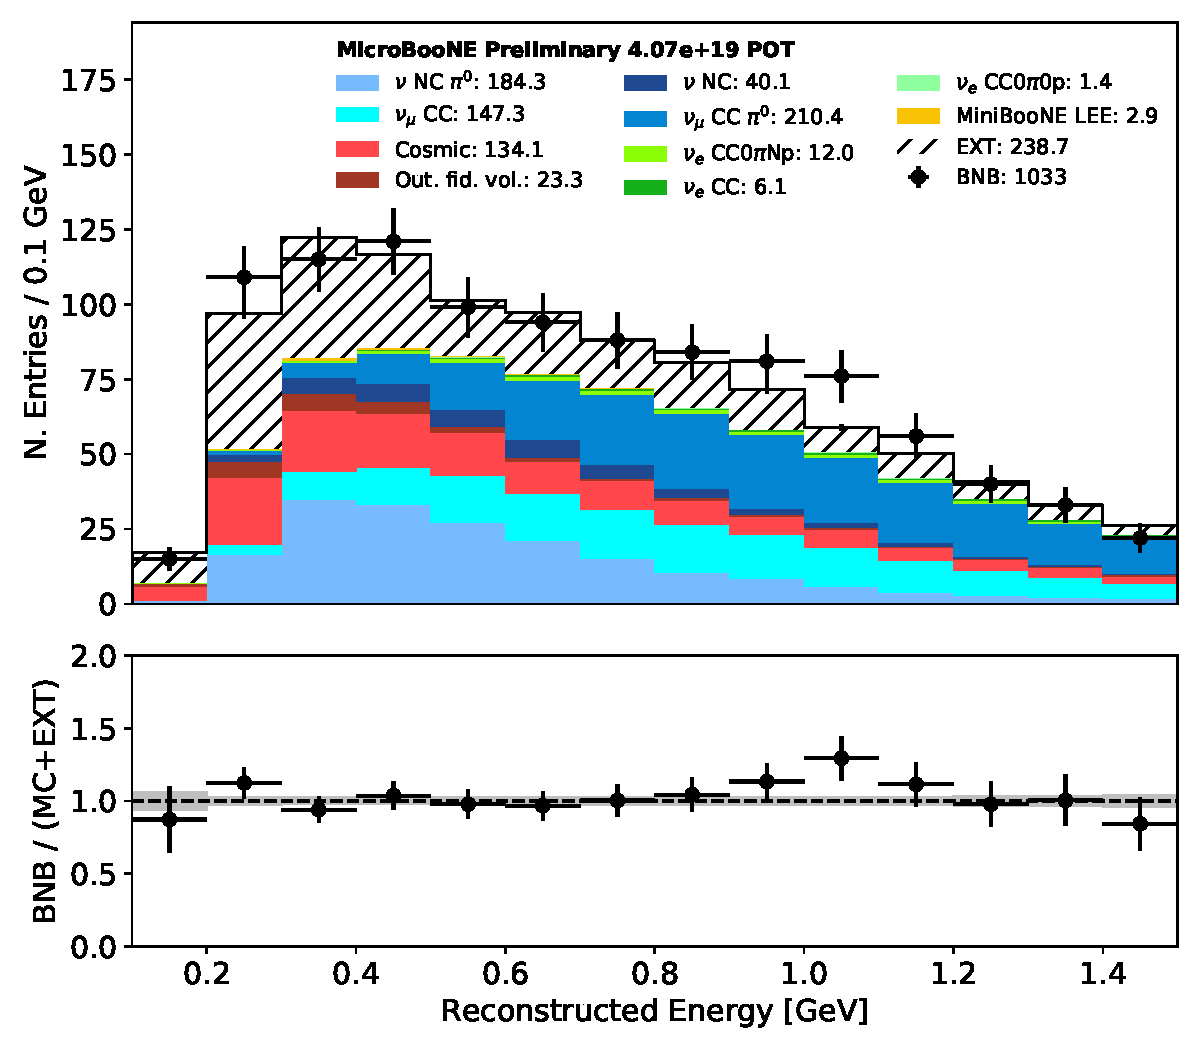
\includegraphics[width=1.00\textwidth]{1eNp/reco_e_01162020_RUN1.pdf}
    \caption{\label{fig:datamccomparisons:nuepresel} \npsel pre-selection for Run  1}
    \end{subfigure}
    \begin{subfigure}[b]{0.44\textwidth}
    \centering
    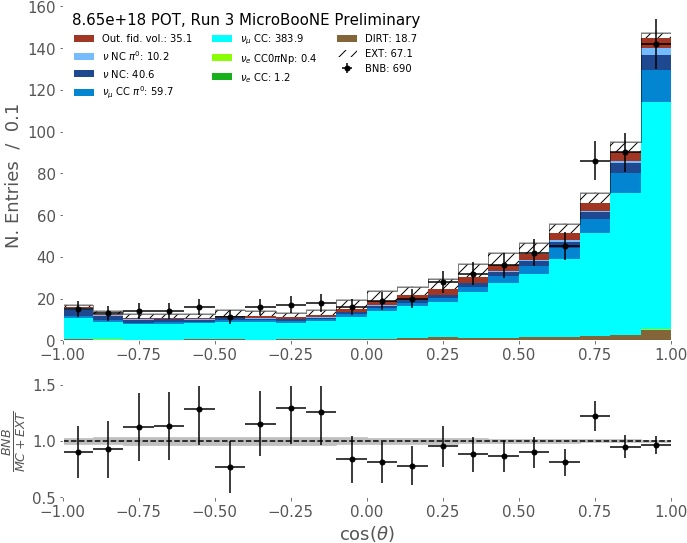
\includegraphics[width=1.00\textwidth]{NuMuCCsel/Images/Ryan/Run3_costheta_withCRT.jpg}
    \caption{\label{fig:datamccomparisons:numu} high-purity $\nu_{\mu}$ for Run 3}
    \end{subfigure}
\caption{\label{fig:datamccomparisons} }
\end{center}
\end{figure}

\par The three $\nu_e$ selections developed in this work all provide strong input to the analysis. Figure~\ref{fig:intro:nueselections} shows the status of the box-cut \npsel (figure~\ref{fig:intro:nueselections:1eNp}), the BDT-based (figure~\ref{fig:intro:nueselections:1e0p}), and the BDT-based $\nu_e$ inclusive (figure~\ref{fig:intro:nueselections:inclusive}). \par The inclusive channel provides the analysis a tool with which to study the modeling of $\nu_e$ interactions, especially at higher energies, and provides a first validation even with the small dataset currently available. Moving forward, we are exploring ways to use this channel to quantitatively constrain high-energy $\nu_e$ modeling uncertainties.
\par The 1$e$0$p$0$\pi$ channel obtains a purity of 49\% and, even though it currently primarily is sensitive to higher-energy $\nu_e$ interactions, provides a valuable validation of detector and modeling effects which can cause migration from the N$p$ to 0$p$ channel. A quantitative estimation of the impact of this channel is being performed.
\par The \npsel channel, in the box-cut selection, achieves a $5-10$\% efficiency with a 73\%  purity for the cut-based  and a $5-15$\% efficiency with a 81\%  purity for the BDT-based selection. These selections lead to $\mathcal{O}$(10) expected MB-$\nu_e$ LEE signal events and $40-70$ intrinsic $\nu_e$ events for the full Run $1-4$ dataset. The final reconstructed energy distribution for the box-cut selection is shown in figure~\ref{fig:intro:nueselections:1eNp}. The box-cut selection's statistics-only sensitivity is $2.1-2.3\sigma$, depending on the test-statistic used. The low statistics of the predicted signals lead to significant fluctuations in the expected sensitivity, covering the range $1.5-3.1\sigma$. 
 \emph{Given the efficiency and purity obtained with the BDT-based workflow, we expect a higher sensitivity compared to the cut-based workflow.  We are in the process of re-evaluating the BDT-based performance which will be reported in this note after higher statistics MC samples have been included, and a re-calibration of the calorimetry has been completed.} 

\begin{figure}[ht] 
\begin{center}
    \begin{subfigure}[b]{0.28\textwidth}
    \centering
    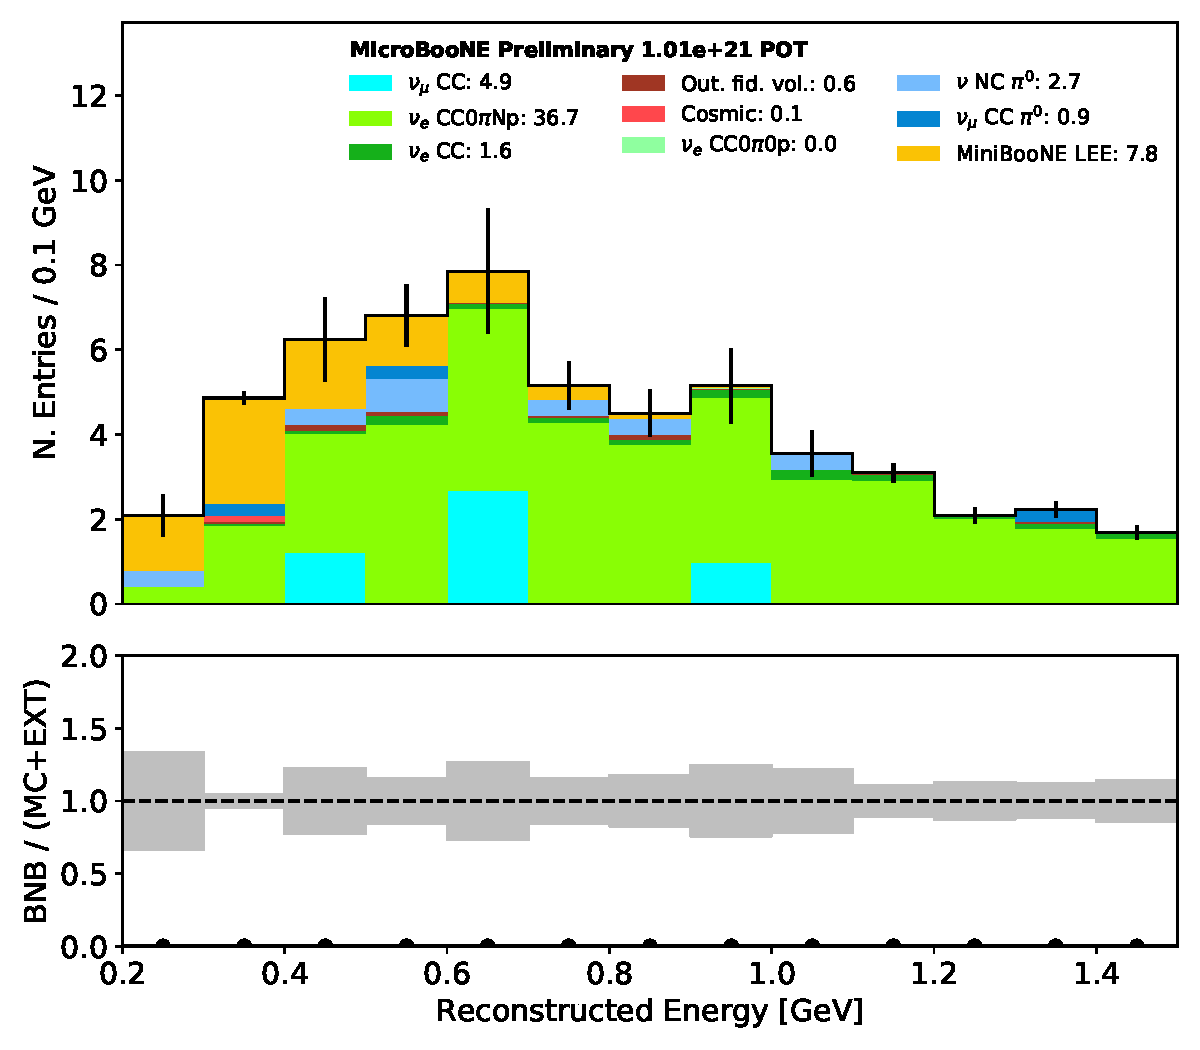
\includegraphics[width=1.00\textwidth]{1eNp/reco_e_01162020_box_RUN1.pdf}
    \caption{\label{fig:intro:nueselections:1eNp} box-cut $\nu_e$ 1$e$0$p$}
    \end{subfigure}
    \begin{subfigure}[b]{0.28\textwidth}
    \centering
    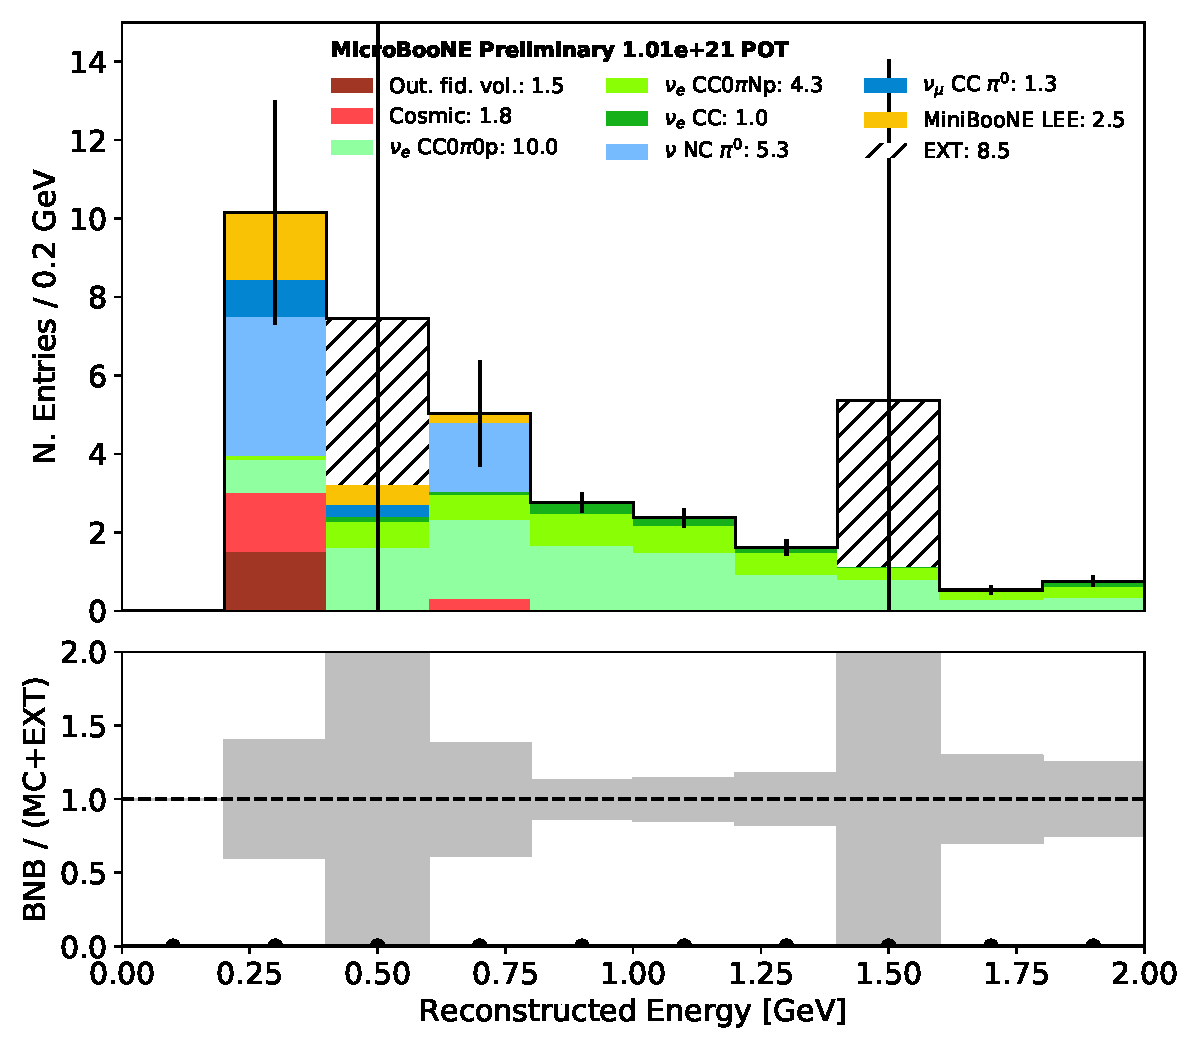
\includegraphics[width=1.00\textwidth]{1e0p/reco_e_01162020_RUN3_bgbdt.pdf}
    \caption{\label{fig:intro:nueselections:1e0p} bdt-based $\nu_e$ 1$e$0$p$}
    \end{subfigure}
    \begin{subfigure}[b]{0.31\textwidth}
    \centering
    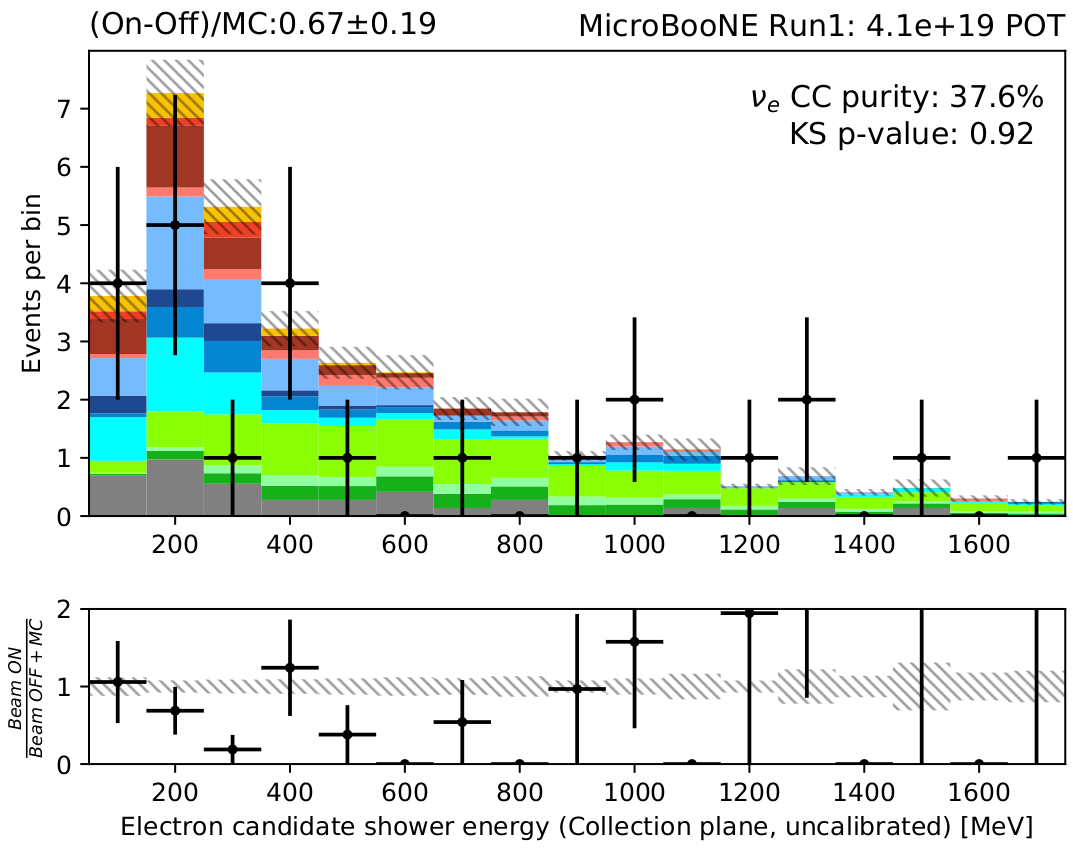
\includegraphics[width=1.00\textwidth]{introduction/nueinclusive.png}
    \caption{\label{fig:intro:nueselections:inclusive} BDT-based $\nu_e$ inclusive}
    \end{subfigure}
\caption{\label{fig:intro:nueselections} }
\end{center}
\end{figure}


\par A particular strength of this analysis consists in the multiple sideband channels available to validate the simulation, reconstruction, and help constrain $\nu_e$ interaction uncertainties. A high statistics $\pi^0$ sideband (section~\ref{sec:controls:pi0}) provides confidence in the performance of the analysis' shower reconstruction. A high-quality inclusive contained $\nu_{\mu}$ selection shows good data-simulation agreement in both Run 1 and Run 3 and provides the input for the $\nu_{\mu}$ constraint which has the primary goal of reducing systematic uncertainties for low-energy $\nu_e$s. A primary estimation of the impact of the $\nu_{\mu}$ constraint shows a 50\% reduction in modeling uncertainties, though this is to be revisited by the time of the February collaboration meeting. Additionally, an inclusive $\nu_{\mu}$ selection (section~\ref{sec:nueselection:inclusive}) provides a valuable starting point for many possible final-state measurements which may become necessary to further validate the analysis as its review progresses. 
\par The full evaluation of systematics for this analysis has not yet been completed. Detector systematic samples available have been investigated and preliminarily show little impact on the selections (sec.~\ref{sec:systematics}) but have not yet been included in sensitivity calculations. The recent availability of an updated central-value simulation for \texttt{GENIE}, together with updated genie modeling uncertainties, will allow us to quantitatively measure the impact of these uncertainties, with and without sideband channel constraints, by the February collaboration meeting. In the meantime, sections~\ref{sec:systematics} and~\ref{sec:sensitivity} present the status of tools and methods used for the full evaluation of the analysis' sensitivity. Statistics-only sensitivity calculations are also presented, based on the box-cut \npsel described in this note.


\newpage

\newpage

\section{Overview of Neutrino Identification}
\label{sec:sliceID}
%\subsection{Event Slicing and Cosmic Removal in Pandora}
The work presented in this note relies on the Pandora event reconstruction~\cite{bib:pandoraub}. Pandora does the low-level pattern-recognition step of the reconstruction, i.e. groups hits into clusters, clusters into particles and particles into hierarchies. This section focuses on the cosmic rejection aspect of the analysis. We describe here how the output of Pandora's pattern-recognition is combined with scintillation light to isolate possible candidate neutrino interactions in MicroBooNE. This process is illustrated in the three images of Figure~\ref{fig:sliceid}. Moreover, we describe how the additional information from the Cosmic Ray Tagger (CRT) is used to improve cosmic rejection in the \numu selection. 

\begin{figure}[ht] 
\begin{center}
    \begin{subfigure}[b]{0.7\textwidth}
    \centering
    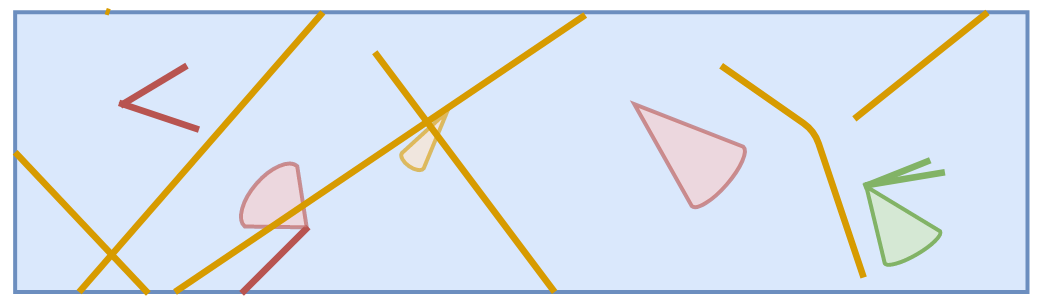
\includegraphics[width=1.00\textwidth]{NuId-Ch3/Images/slice00.png}
    \caption{\label{fig:slcieid:00} Typical event with multiple interactions isolated by Pandora in \texttt{slices}. Candidate neutrino interactions are shown in green and red.  Obvious cosmics are shown in orange.}
    \end{subfigure}
    \begin{subfigure}[b]{0.7\textwidth}
    \centering
    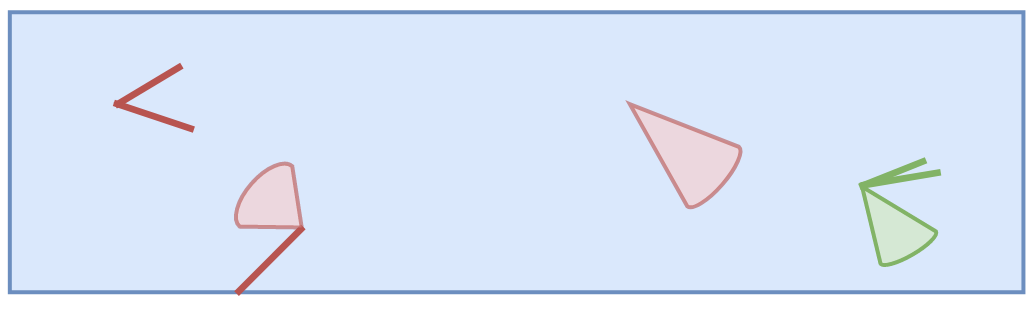
\includegraphics[width=1.00\textwidth]{NuId-Ch3/Images/slice01.png}
    \caption{\label{fig:slcieid:01} Event after the removal of \texttt{obvious cosmics} tagged geometrically by Pandora.}
    \end{subfigure}
    \begin{subfigure}[b]{0.7\textwidth}
    \centering
    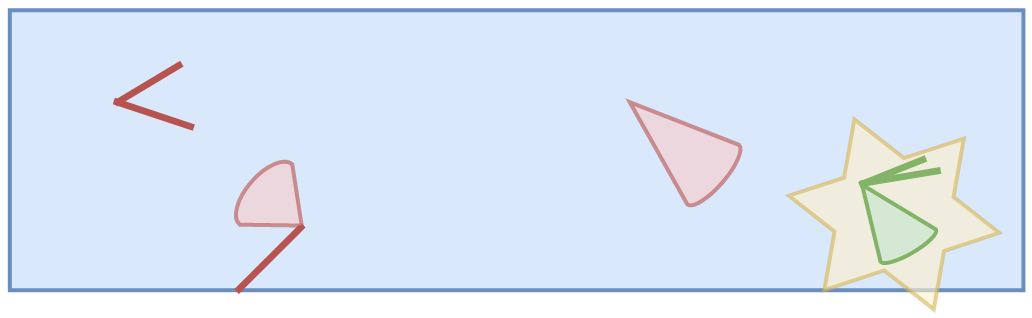
\includegraphics[width=1.00\textwidth]{NuId-Ch3/Images/slice02.png}
    \caption{\label{fig:slcieid:02} Implementation of the \texttt{SiceID} tool to isolate possible candidate $\nu$ interactions.  The selected candidate is highlighted, and shown in green.}
    \end{subfigure}
\caption{\label{fig:sliceid} Succession of steps in cosmic removal performed using Pandora's topological pattern recognition combined with scintillation light information through the \texttt{NeutrinoID} tool.}
\end{center}
\end{figure}

%\subsection{Slicing, Clustering and Vertexing}
\subsection{Pandora Slicing, Clustering and Vertexing}
The creation of a ``slice" is the first step of the Pandora processing. A slice is a collection of distinct reconstructed particles which belong to the same interaction, such as a cosmic muon and its Michel electron, or the muon and proton in a 1$\mu$1$p$ neutrino interaction. To produce slices, the Pandora cosmic pattern recognition is first run over all hits, aiming to construct muon tracks and any associated $\delta$-rays or Michel electrons under the cosmic hypothesis (fig.~\ref{fig:slcieid:00}). At this stage, obvious cosmic activity (through-going or out-of-time muons) is tagged using geometric information and discarded (fig.~\ref{fig:slcieid:01}). The remaining hit collection is used as input to Pandora and reconstructed both under the cosmic hypothesis and the neutrino hypothesis. A typical event contains approximately five slices at this stage. 

%\subsubsection{Clustering and Vertex Finding } 
\par In order to reconstruct the interactions in three dimensions, Pandora needs to match the information from at least two different views and create a neutrino vertex. Pandora performs the 2D clustering on the hits in each slice and on each plane separately. Then a number of 3D candidate vertices is created by finding positions that project down onto the ends of the available 2D clusters. All of the possible vertex candidates are fed into the support vector machine (SVM) vertex selection, and the candidate with the highest SVM score is chosen. This 3D vertex is used to split any existing clusters that cover the vertex. Then the cluster matching algorithms are run; in these algorithms the clusters are compared between views and modified to improve the matching.

\subsection{Pandora NeutrinoID: Cosmic Removal Via Topology and Scintillation Light}
\label{sec:sliceID:NeutrinoID}
\par After the set of Pandora pattern-recognition algorithms has isolated individual interactions into reconstructed slices and removed obvious cosmics, the remaining task is to identify which slice, if any, is associated with a neutrino interaction. Scintillation light information is used to reject slices incompatible with light recorded in-time with the beam. Topological cuts aimed at rejecting stopping-muon events which enter the TPC are also used. The \texttt{NeutrinoID} is at the core of all neutrino selections performed in this analysis; this first, common step is responsible for the majority of cosmic-rejection.
\\
\par We leverage three handles to distinguish between neutrino and cosmic-ray slices:
\begin{enumerate}
    \item Simple optical pre-selection cuts, which remove slices inconsistent with the beam flash;
    \item A topological score which assesses to what extent the slice looks like a neutrino interaction in the TPC (see DocDB 14175)
    \item A flash-matching score, which assesses how well the flash-hypothesis for the slice matches the beam flash.
\end{enumerate}

To select the neutrino slice, we first require a beam-triggered flash in the beam window. Then we apply the optical pre-selection cuts. If no slice passes optical pre-selection, the event is rejected. If the slice with the largest topological score passes the optical pre-selection, the slice forms the neutrino candidate; otherwise, the slice with the largest  flash-matching score forms the neutrino candidate. 
The performance of the \texttt{NeutrinoID} for simulated neutrino events is shown in~\cref{fig:sliceid_eff}.
Integrated over all final states and neutrino energies, the efficiency is:
\begin{itemize}
    \item[-] $\nu_\mu$ charged-current: \SI{83.0}{\%}
    \item[-] $\nu_e$ charged-current: \SI{83.3}{\%}
\end{itemize}
Further details on the \texttt{NeutrinoID} tool are available in DocDB 28418, 23854 and 22519.

\begin{figure}[H]
    \centering
    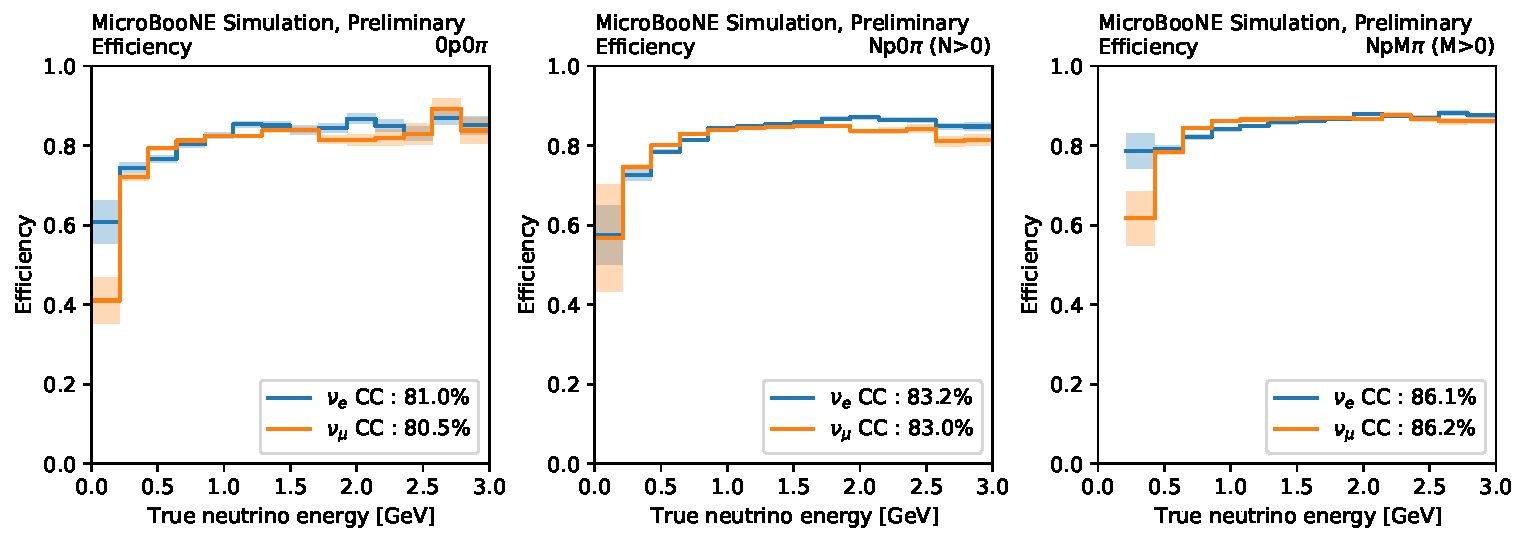
\includegraphics[width=0.75\textwidth]{NueCCsel/Images/truth/sliceID_eff.pdf}
    \caption{The performance of the \texttt{NeutrinoID} tool as a function of the true neutrino energy for the topologies considered in the \nuecc selection: \zpsel (left), \npsel (middle) and inclusive (right) channels. The energy range is \SIrange{0}{3}{\GeV} and the bin size is \SI{200}{\MeV}. The shaded areas correspond to the statistical errors arising from limiter simulated sample sizes.}
    \label{fig:sliceid_eff}
\end{figure}



\subsection{CRT Veto and Distance Tagger}
\label{sec:sliceID:CRT}
CRT tools are used in this analysis to boost cosmic rejection in the $\nu_{\mu}$ constrain selection, where the analysis-level containment requirement removes the concern of tagging exiting muons through CRT-based cuts. CRT-based cuts were explored for the $\nu_e$ selections as well but were ultimately found to be of little impact in the \npsel due to the powerful cosmic rejection achieved when requiring final-state protons. Considerable additional cosmic rejection was obatined with the CRT in the \zpsel, but the current analysis has chosen to not implement these cuts to avoid complications in mixing datasets from different runs with different selection requirements. Two specific cut concepts have been developed to make use of CRT information. Both are used in the $\nu_{\mu}$ and are described below.

\textbf{CRT Veto.} The CRT veto looks for a time coincidence between the scintillation light recorded in time with the 1.6 $\mu$s beam-spill (beam flash) and a CRT hit: if a CRT hit occurs within 1 $\mu s$ of the beam flash, the event is rejected. For this coincidence, only CRT hits with PE $>$ 100 p.e. are considered; we do not apply a constraint on the position of the flash or on the position of the CRT hit. 
The rejection power and efficiency of the CRT veto are calculated using the BNB external and the $\nu_e$ overlay samples, respectively. The BNB external rejection rate is $\sim$59\%. %,  and the $\nu_e$ passing rate greater than $\sim$94\% for all electron neutrino energies, even higher at low energies. \\

\textbf{CRT Distance Tagger.} 
The CRT Distance Tagger tool builds upon the standard Pandora neutrino vertex reconstruction and the CRT tagging of TPC tracks. A TPC track is tagged with a CRT hit association if the track projection onto a CRT panel and a CRT hit are close in space. 
To perform this association, the track projection to the CRT is calculated under the hypothesis that the associated particle crossed the TPC at the time registered by the CRT hit under consideration. More details on the CRT hit to TPC track matching are available in \cite{bib:CRTPresel_Technote}.  The CRT Distance Tagger checks the minimum distance between the reconstructed neutrino vertex and each track tagged with a CRT hit. If the minimum distance is less than 14 cm, the event is rejected. An example event tagged by this cut is shown in Figure~\ref{fig:crtdist00}.  With the CRT Distance Tagger an additional 19\% of off-beam backgrounds are rejected.% external passing rate is $\sim$81\%,  and the $\nu_e$ efficiency is greater than $\sim$96\% for all electron neutrino energies, even higher at low energies. \\
 
\begin{figure}[h!]
\centering
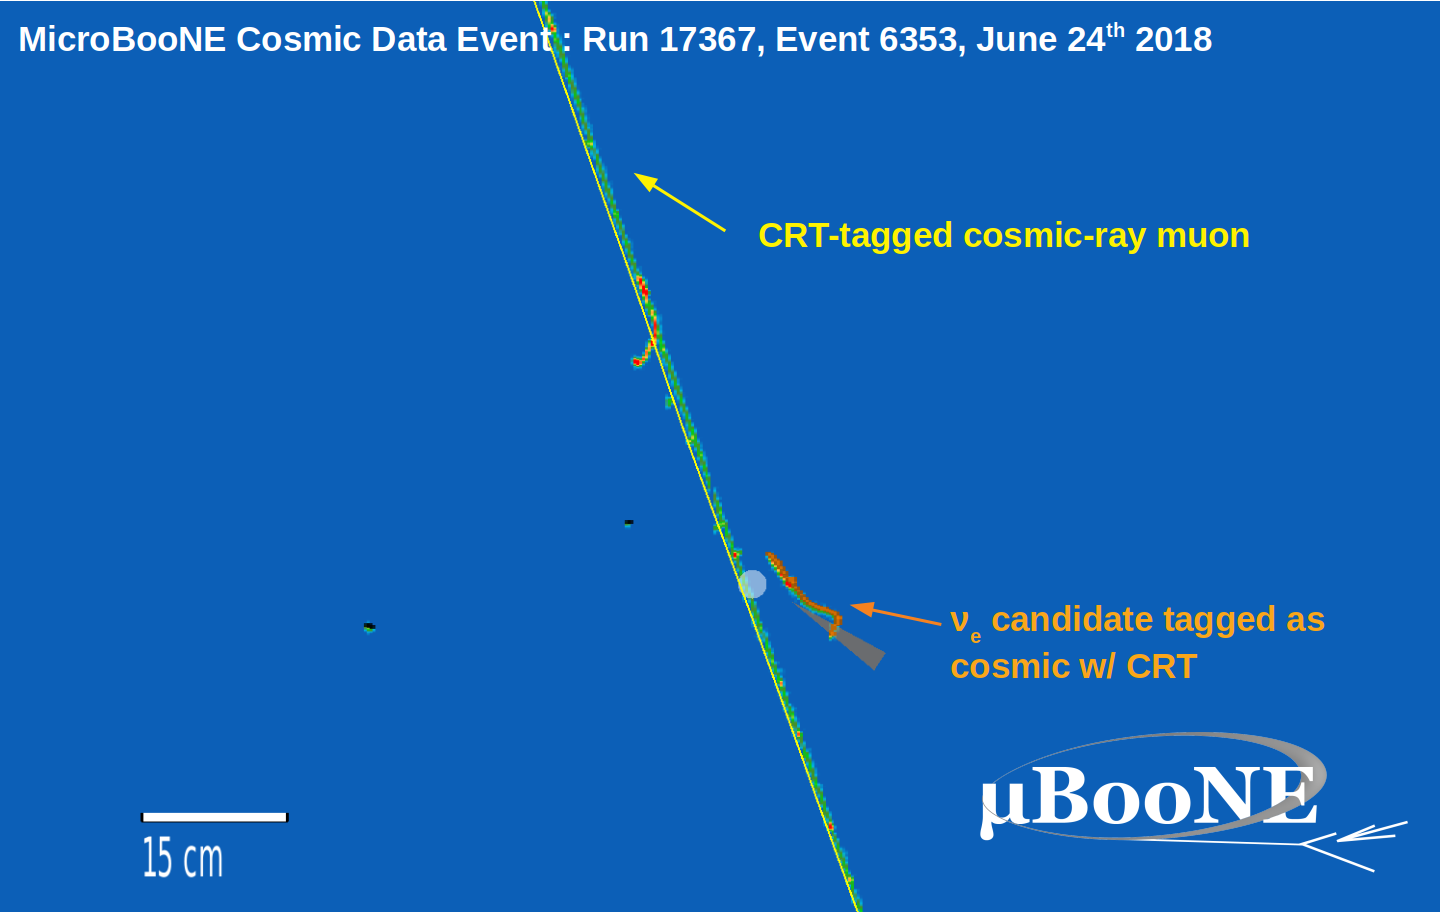
\includegraphics[width=0.4\textwidth]{NuId-Ch3/Images/crttagger_01.png}
\caption{Example $\nu_e$ candidate tagged as cosmic by the the CRT distance tagger. From the event one can see that the reconstructed EM shower is from EM activity that is associated with the cosmic muon.}
\label{fig:crtdist00}
\end{figure}

An overview of the impact of the CRT on cosmic rejection can be seen in Figure~\ref{fig:crt} where the beam-time distribution for the 8E18 POT Run 3 open data set is shown just after \texttt{NeutrinoID} (left), and after both \texttt{NeutrinoID} and CRT cosmic-tagging tools (including the CRT veto and distance tagger) have been applied (right). The EXT backgrounds drop by more than a factor of three.
Further details and a preliminary study of the CRT  impact on an electron neutrino pre-selection can be found in \cite{bib:CRTPresel_Technote}. 

\begin{figure}[ht] 
\begin{center}
    \begin{subfigure}[b]{0.4\textwidth}
    \centering
    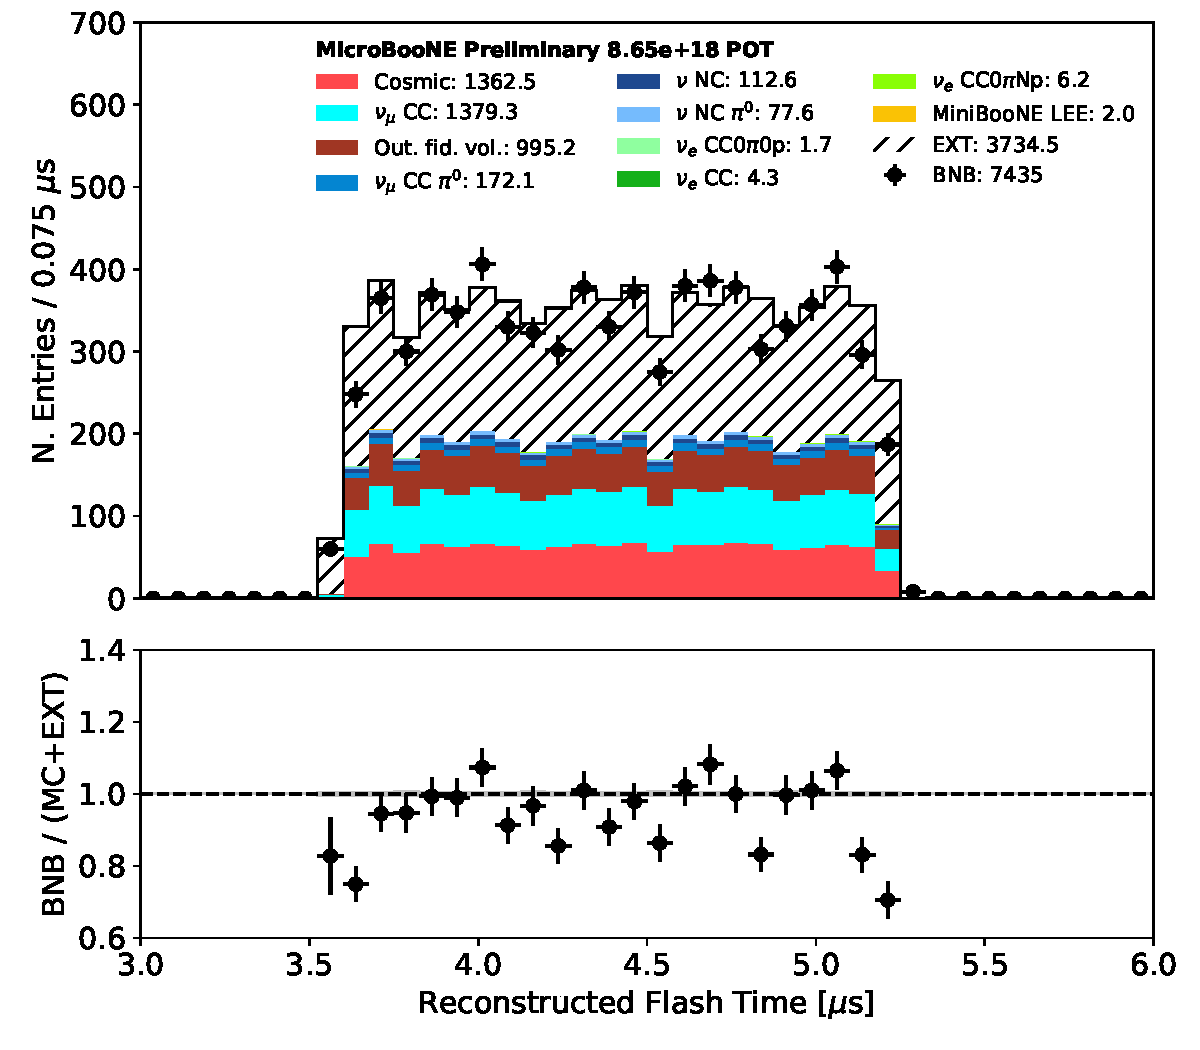
\includegraphics[width=1.00\textwidth]{NuId-Ch3/Images/flash_time_01152020.pdf}
    \caption{\label{fig:crt:pre} No CRT tools.}
    \end{subfigure}
    \begin{subfigure}[b]{0.4\textwidth}
    \centering
    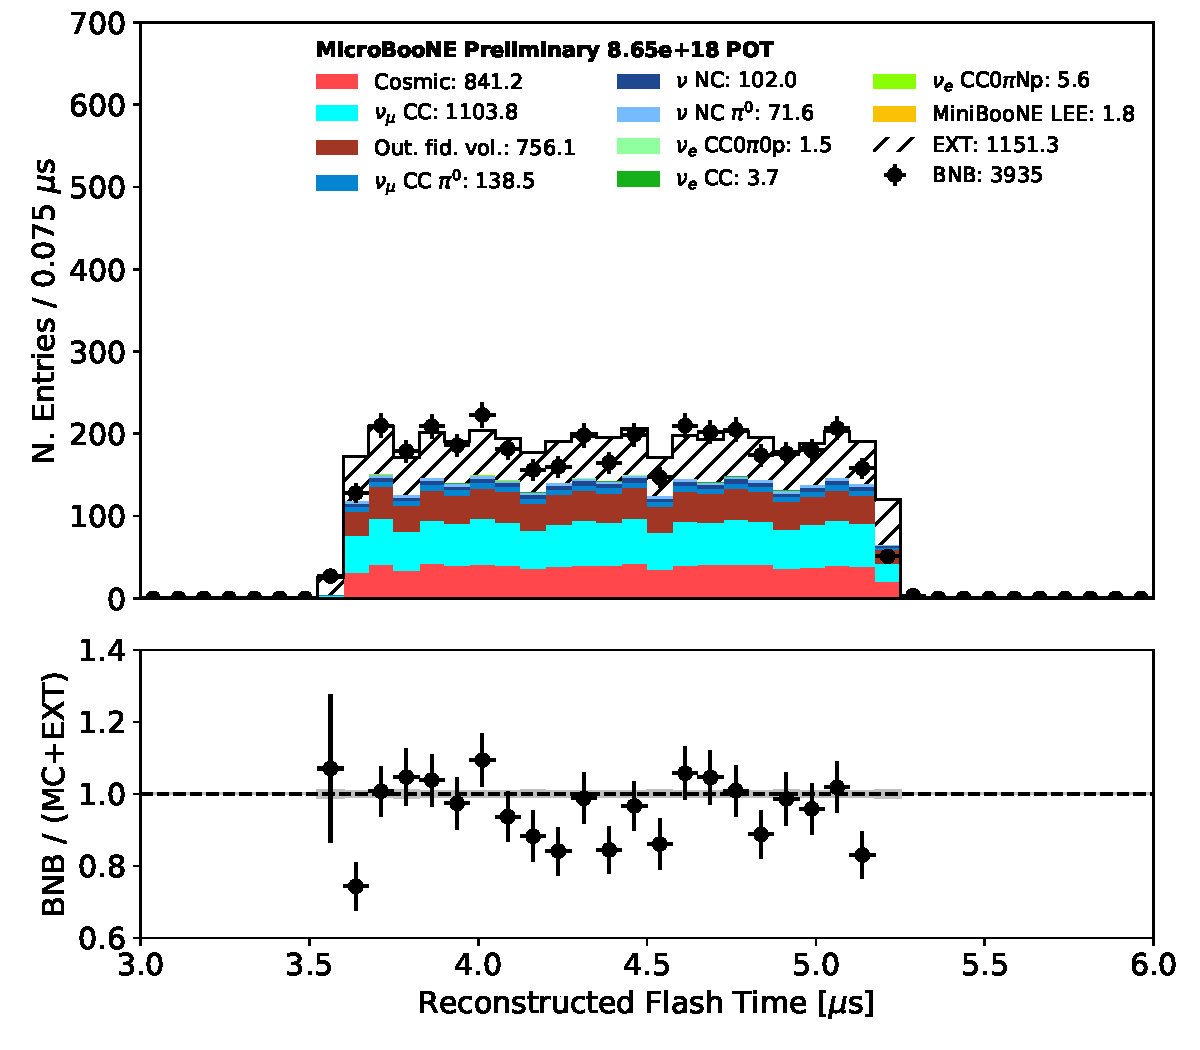
\includegraphics[width=1.00\textwidth]{NuId-Ch3/Images/flash_time_01152020_CRT.pdf}
    \caption{\label{fig:crt:post} With CRT tools.}
    \end{subfigure}
\caption{\label{fig:crt} Beam timing distribution before (a) and after (b) CRT tools have been applied. The EXT contribution is reduced by over a factor of three.}
\end{center}
\end{figure}

\newpage

\section{Neutrino Event Reconstruction}
\label{sec:NuEvtReco}
This section highlights the key aspects of the event reconstruction which allow for the classification of neutrino interactions: the track and shower reconstruction, the particle identification and the energy reconstruction.
\subsection{Track and Shower Reconstruction}
\label{sec:tkshreco}
The output of Pandora~\cite{bib:pandoraub} is organized in a hierarchy of reconstructed Particle Flow Particles (``PFParticles''), which describes the particle content in an observed event as a parent-daughter relationship chain. Final state PFParticles are 3D objects matching clusters of hits in at least two different planes.
Pandora classifies PFParticles as track-like or shower-like base on a Support Vector Machine (SVM) algorithm~\cite{bib:tkshsvm}, producing a score with values between 0 (shower-like) and 1 (track-like). PFParticles will be collected together based on physical proximity into slices, and ordered in a hierarchy (i.e. a Michel electron is the daughter of a muon, which is a daugther of a neutrino).

Pandora processes track-like PFParticles with a sliding linear fit procedure (described in~\cite{bib:pandoraub}) that returns the 3D position and direction at each point along the trajectory (where each point corresponds to a 2D hit). For each point the d$Q$/d$x$ and distance from the track-start are recorded using MicroBooNE's Calorimetry module. This procedure allows to accurately measure both d$x$, including small deflections due to the particle's trajectory and Space Charge Effect (SCE) offsets, and d$Q$, by incorporating MicroBooNE's full position- and field-dependent relative and absolute charge calibration. For tracks, the conversion from d$Q$/d$x$ to d$E$/d$x$ is performed by applying the inverse Modified Box recombination model~\cite{bib:tpccalibrationnote}.

We evaluate the energy and 3D direction of shower-like PFParticles with the same algorithm used for the $\pi^0$ reconstruction paper~\cite{bib:pi0reco}. The energy reconstruction accounts for various detector effects, including gain and recombination; corrections for reconstruction effects (hit threshold and imperfect clustering) will be described in Sec.~\ref{sec:ereco}. We also fit showers using a Kalman filter-based procedure~\cite{bib:shrtrackfitter} which aims at identifying the main trunk of the shower by rejecting hits that are longitudinally or transversely displaced from it; the output of this fit is a track object. Thus, the calorimetric tools described above become available for showers as well, with an important caveat: the conversion from d$Q$/d$x$ to d$E$/d$x$ is different for showers and tracks. For showers, a fixed recombination correction is applied assuming 2.1 MeV/cm energy loss for both the calculation of the trunk d$E$/d$x$ and for the total energy. In all cases, local variations in the electric field are accounted for.

By default, Pandora separates showers and tracks with a cut on the SVM score at 0.5; however, as will be described in later sections, in many cases we choose different cut values, i.e. tighter shower definition for the $\nu_e$ selection and looser for the $\pi^0$ control region.

The efficiency of Pandora's reconstruction on $\nu_e$ interactions is evaluated in figure~\ref{fig:nuereco:eff} as a function of true neutrino energy;  the efficiency for identifying the $\nu_e$ events as neutrino interactions is shown in black, and the efficiency for reconstructing $\nu_e$ interactions with a final-state EM shower in blue. The efficiency has a sharp upturn between 100 and 200 MeV, especially in the case when an EM shower is required, and levels off at 80\% and 60\% respectively for the two curves. 
\par At this stage in the analysis, the good efficiency for reconstructing $\nu_e$ events is offset by the very low signal-to-background for $\nu_e$ events in MicroBooNE's data, a consequence of the very small $\nu_e$ content of the beam. With no additional requirement on the reconstructed neutrino, the purity for $\nu_e$ interactions is 0.12\% (figure~\ref{fig:nuereco:sliceid}). After imposing a requirement of one reconstructed shower, the purity grows by almost an order of magnitude, to 1\% (figure~\ref{fig:nuereco:shower}). The $\nu$ background composition also changes significantly, with $\pi^0$ backgrounds moving from 14\% to 48\% of all backgrounds.

\begin{figure}[ht] 
\begin{center}
    \begin{subfigure}[b]{0.3\textwidth}
    \centering
    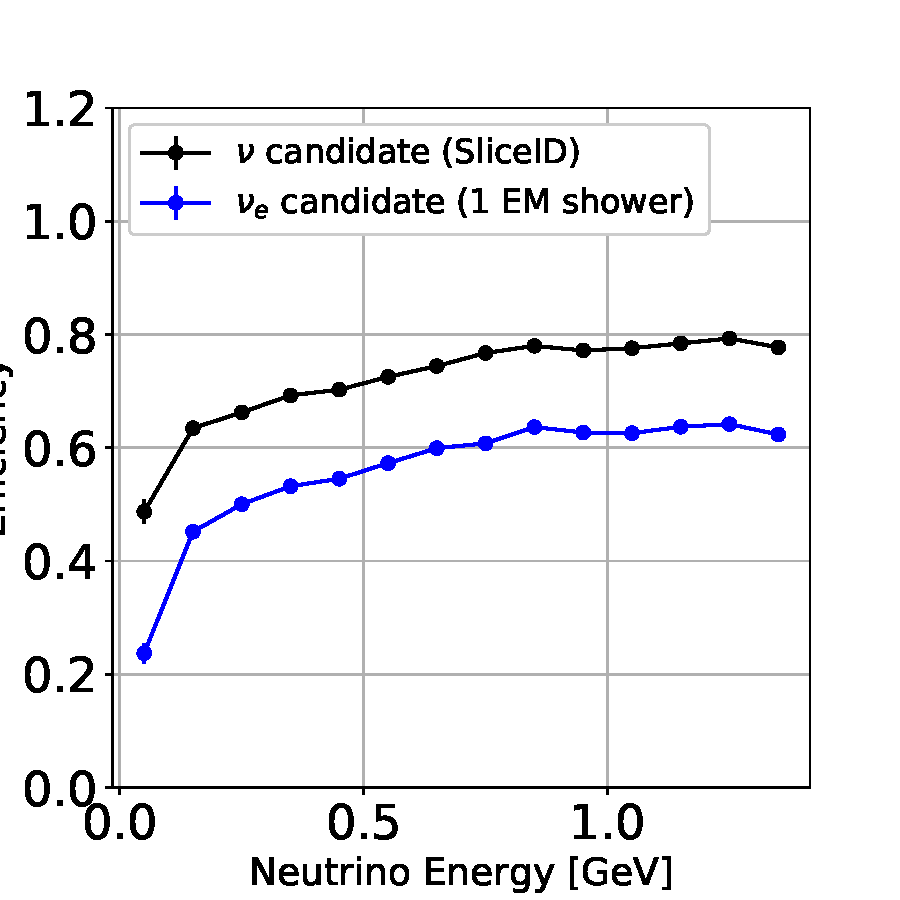
\includegraphics[width=1.00\textwidth]{nureco/nureco_RUN1.pdf}
    \caption{\label{fig:nuereco:eff} $\nu_e$ reco eff.}
    \end{subfigure}
    \begin{subfigure}[b]{0.31\textwidth}
    \centering
    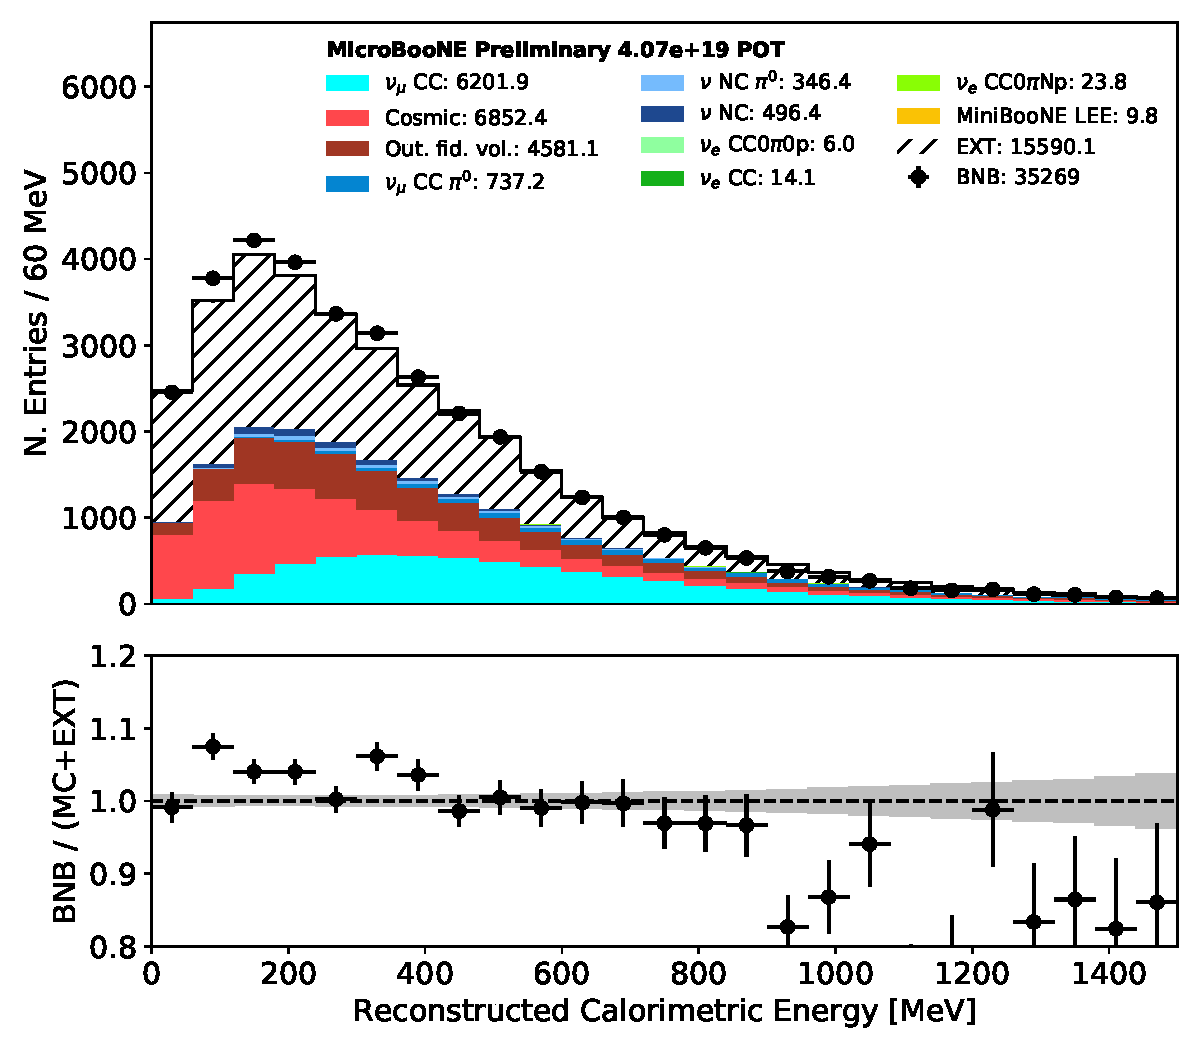
\includegraphics[width=1.00\textwidth]{nureco/NeutrinoEnergy2_01152020.pdf}
    \caption{\label{fig:nuereco:sliceid} after \texttt{SliceID}}
    \end{subfigure}
    \begin{subfigure}[b]{0.31\textwidth}
    \centering
    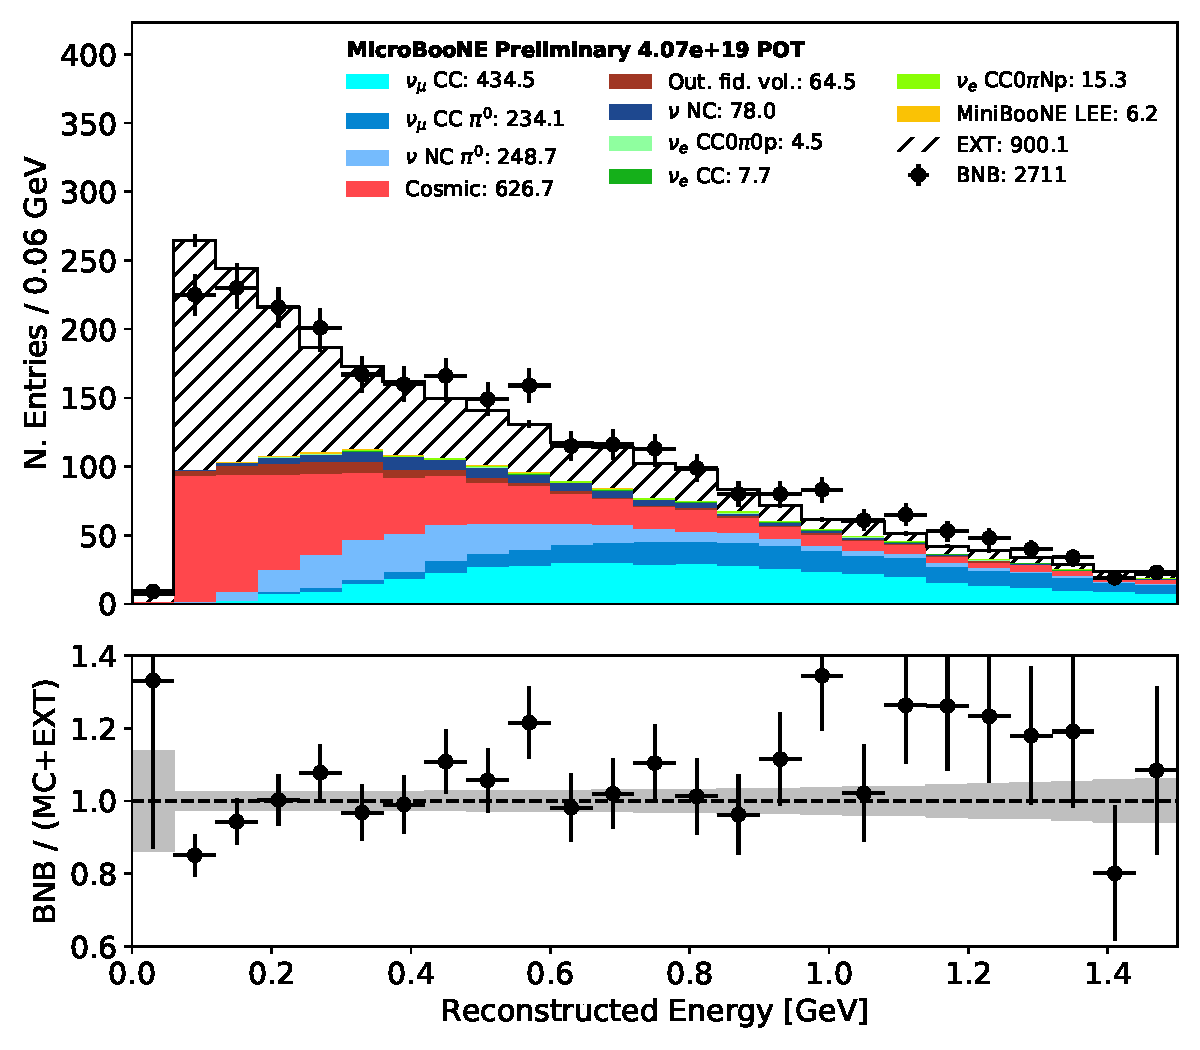
\includegraphics[width=1.00\textwidth]{nureco/reco_e_01152020.pdf}
    \caption{\label{fig:nuereco:shower} after shower requirement}
    \end{subfigure}
\caption{\label{fig:nuereco} \textcolor{blue}{ Y axis of figure a is cut off}}
\end{center}
\end{figure}

\par The next step in the analysis demands the development of a selection capable of isolating $\nu_e$ interactions rejecting the two order of magnitude larger background rates from $\nu_{\mu}$ neutrinos. This selection will make use of PID and topological information described in the next sections. The strong level of background rejection needed to isolate signal events will inevitably lead to a lower selection efficiency.

\subsection{Particle Identification}
% GC: this part is now in the previous subsection
%In the neutrino slice, every PFParticle is reconstructed in three different ways:
%\begin{itemize}
%    \item Track, using the standard Pandora Track reconstruction
%    \item Shower, using the standard Pandora Shower reconstruction (is there any modification on top of this?)
%    \item Track-fitted shower, using a dedicated track fitting tool which aims at identifying the main branch of %the shower and fit it as a track. As a result, all the tools developed for the track become available for the %tracks too. For example, for each track-fitted shower, a recob::track and a anab::calorimetry objects are available.
%\end{itemize}
Particle identification is performed with different tools depending on whether the particle is selected as a track- or shower-candidate.
If the PFParticle has been selected as a track-like object, the identification is performed using the Calorimetry Likelihood tool, which results in the variable Log Likelihood Ratio PID (LLR), see section~\ref{subsec:loglikelihoodpid}.
If the PFParticle has been selected as an electron or photon candidate, the identification is performed using several variables described in \ref{subsec:egammaspearation}.
%It is noteworthy that this particle identification consists of one or multiple variables, available for the specific PFParticle, that may or may not depend on \textcolor{blue}{additional information from} the rest of the slice. 
%For example, the shower d$E$/d$x$ depends only on the PFParticle itself, whereas the track-shower separation relies also on additional objects identified in the slice.
Notably, additional information provided by the rest of the slice may be used for the particle identification 
depending on the specific PFParticle. For example, while the shower d$E$/d$x$ depends only on the PFParticle itself, the track-shower separation relies also on additional objects identified in the slice.

When choosing the cut values for PID variables, we account not only for the efficiency and mis-identification achievable to distinguish two kinds of particles (e.g. electrons from photons), but also for the mixture of backgrounds specific to the considered topology: e.g. \textcolor{blue}{add example}. 

%The value of the cuts applied on these variables depends not only on the general level of efficiency and mis-identification achievable to distinguish two kind of particles (electrons from photons, for example), but also on the mixture of backgrounds specific to selection the analyzer is performing.





\subsubsection{Log Likelihood Ratio  PID \textcolor{green}{Nico, P.R. David, Elena}}
\label{subsec:loglikelihoodpid}

For track-like particles, the particle identification is performed looking at the profile of the deposited charge per unit length (d$E$/d$x$). The scope of track PID is to identify the particle type which originated a given track object. In this analysis, we limit PID to a binary classification problem, i.e.  how to distinguish protons from muons. We disregard further classification because kaons are rarely produced in neutrino interactions at the energy of interest, whereas pions are very difficult to distinguish from muons using calorimetry information only.
Additional information, such as possible hadronic reinteractions or Michel electrons, can be powerful to perform particle identification but is not leveraged in this analysis.

The expected distribution of the $dE/dx$ is modeled for each particle type and for each plane, as a function of two variables: the residual range ($rr$), and the pitch as
\[ p(dE/dx | \text{type}, \text{plane}, \text{rr}, \text{pitch}). \]
The residual range is the distance of a given space point from the end of the track, measured along the track trajectory, while the pitch is the length over which the charge measured on a given wire has been deposited.
The expected distribution is modeled for each plane independently, and for the two kinds of particles under study, protons and muons.
Multiple effects enter in the model of this distribution.
The first effect is what we want to leverage:  the average d$E$/d$x$ at a given residual range depends on the particle's mass, as seen by integrating the Bethe-Bloch function for different masses.
Secondly, the fluctuations of the d$E$/d$x$ depend on the pitch. These fluctuations are intrinsically stochastic: the longer the length over which the charge is averaged, the smaller the fluctuations.
Furthermore, detector effects such as recombination, signal deconvolution, and hit reconstruction add a non-linear response and smearing; this response depends on both the true deposited charge and the pitch, and lacks an analytic model. For this reason, the expected distribution of $dE/dx$ is built starting from the simulation.
The performance of the particle identification improves as the model for the  $dE/dx$ distribution becomes more accurate.
The model for $dE/dx$ is built by considering well reconstructed tracks\footnote{ We define a ``well reconstructed track" a track whose completeness and purity are both above 90\%, where completeness measures how much of the true particle's  deposited charge is reconstructed in the track and purity measures how little spurious charge enters the track reconstruction. }, well contained within a fiducial volume, and backtracked to protons and muons.
The binning of the probability density function (pdf) is the following:
\begin{itemize}
    \item $dE/dx$: $[0, 0.5, 1, 1.5, 2, 2.5, 3, 3.5, 4, 4.5, 5, 5.5, 6, 6.5, 7, 7.5, 8, 9, 10, 12, 15, 20, 25, 30, 35, 40, 45, 50]$ MeV/cm
    \item residual range: $[0., 2, 4, 7, 10, 15, 20, 30, 50, 100, 300, 2000]$ cm
    \item pitch: $[0.3, 0.6, 1, 1.5, 3, 30]$ cm
\end{itemize}
A couple of examples of the pdf are provided in figure \ref{fig:llr_pid_pdf_example}, for two different bins in residual range and pitch.

\begin{figure}[ht] 
\begin{center}
    \begin{subfigure}[b]{0.48\textwidth}
    \centering
    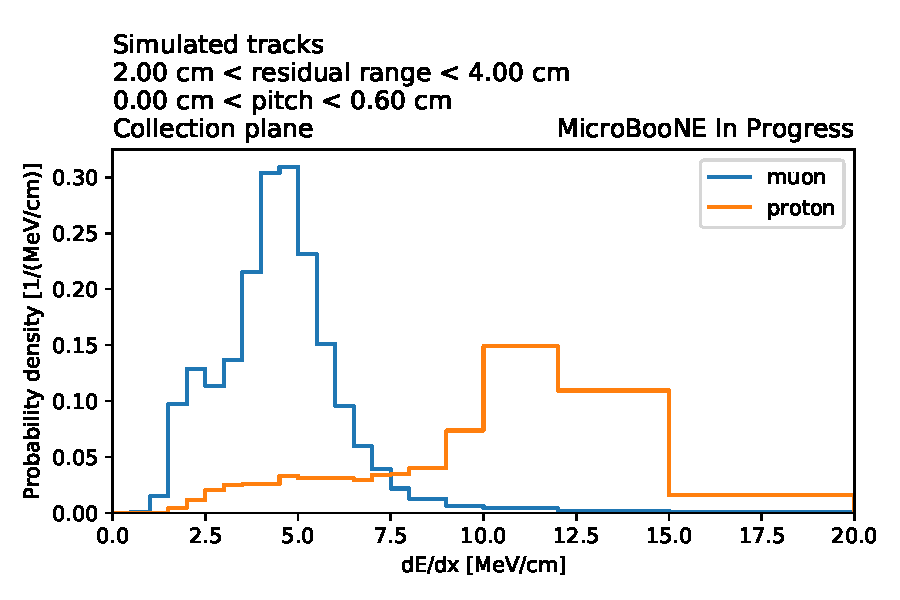
\includegraphics[width=1.00\textwidth]{llrpid/plane_2_rr_30_pitch_03.pdf}
    \end{subfigure}
    \begin{subfigure}[b]{0.48\textwidth}
    \centering
    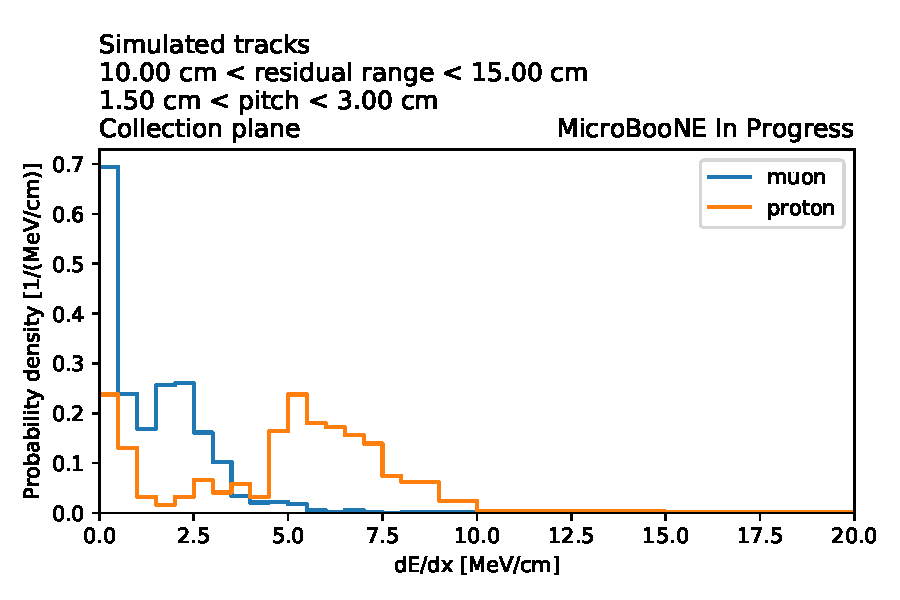
\includegraphics[width=1.00\textwidth]{llrpid/plane_2_rr_125_pitch_225.pdf}
    \end{subfigure}
\caption{Comparison of the expected distribution of $dE/dx$ for muons (blue) and protons (orange), for two different bins in residual range and pitch (left and right).}
\label{fig:llr_pid_pdf_example}
\end{center}
\end{figure}

For a given track, we consider the calorimetry objects on all three planes. For each plane, the $dE/dx$, residual range, and pitch vectors are used to compute the likelihood of each particle type,
\[ \mathcal{L}(\text{type} | \text{plane}, dE/dx_{i = 1, ..., N},   \text{rr}_{i = 1, ..., N}, \text{pitch}_{i = 1, ..., N}) = \prod_{i=1}^N p(dE/dx_i | \text{type}, \text{plane}, \text{rr}_i, \text{pitch}_i) \]
where the index $i=1, ..., N$ runs over each hit for the considered plane.
The combination of the three planes happens in a straightforward way, by taking the product of the three likelihoods, or summing up the log-likelihoods,
\[ p(dE/dx | \text{type}, \text{plane}, \text{rr}, \text{pitch}). \]
In order to perform the classification task, the likelihood ratio test statistic is chosen:
\[ T(dE/dx, \text{rr}, \text{pitch}) = \mathcal{L}(\text(muon)| dE/dx, \text{rr}, \text{pitch}) /  \mathcal{L}(\text(proton)| dE/dx, \text{rr}, \text{pitch}). \]
An example of the distribution of these variable, normalized between -1 and 1, is given in figure \ref{fig:llr_pid_uvy_example}, for tracks contained in a fiducial volume, and backtracked to muon, proton, or cosmic.

The likelihood ratio, as defined above can be proven to be the most powerful statistical test, i.e. the one with the smallest mis-identification rate for any given value of the efficiency.
Any mis-modeling in the simulation used to build the likelihood produces a loss of power, as the test would not be the most powerful one.
Systematic uncertainties arise from the fact that the measured distribution of $dE/dx$ in the data may differ from the simulation, or because the properties of the tracks we consider may not be properly simulated, such as angular or length distributions.
This behaviour is qualitatively present in all the PID methods.

In a MC sample of contained protons and muons used to test the performance, this PID variable is able to reach 94\% muon efficiency, with 10\% proton mis-ID rate.

\begin{figure}[ht] 
    \centering
    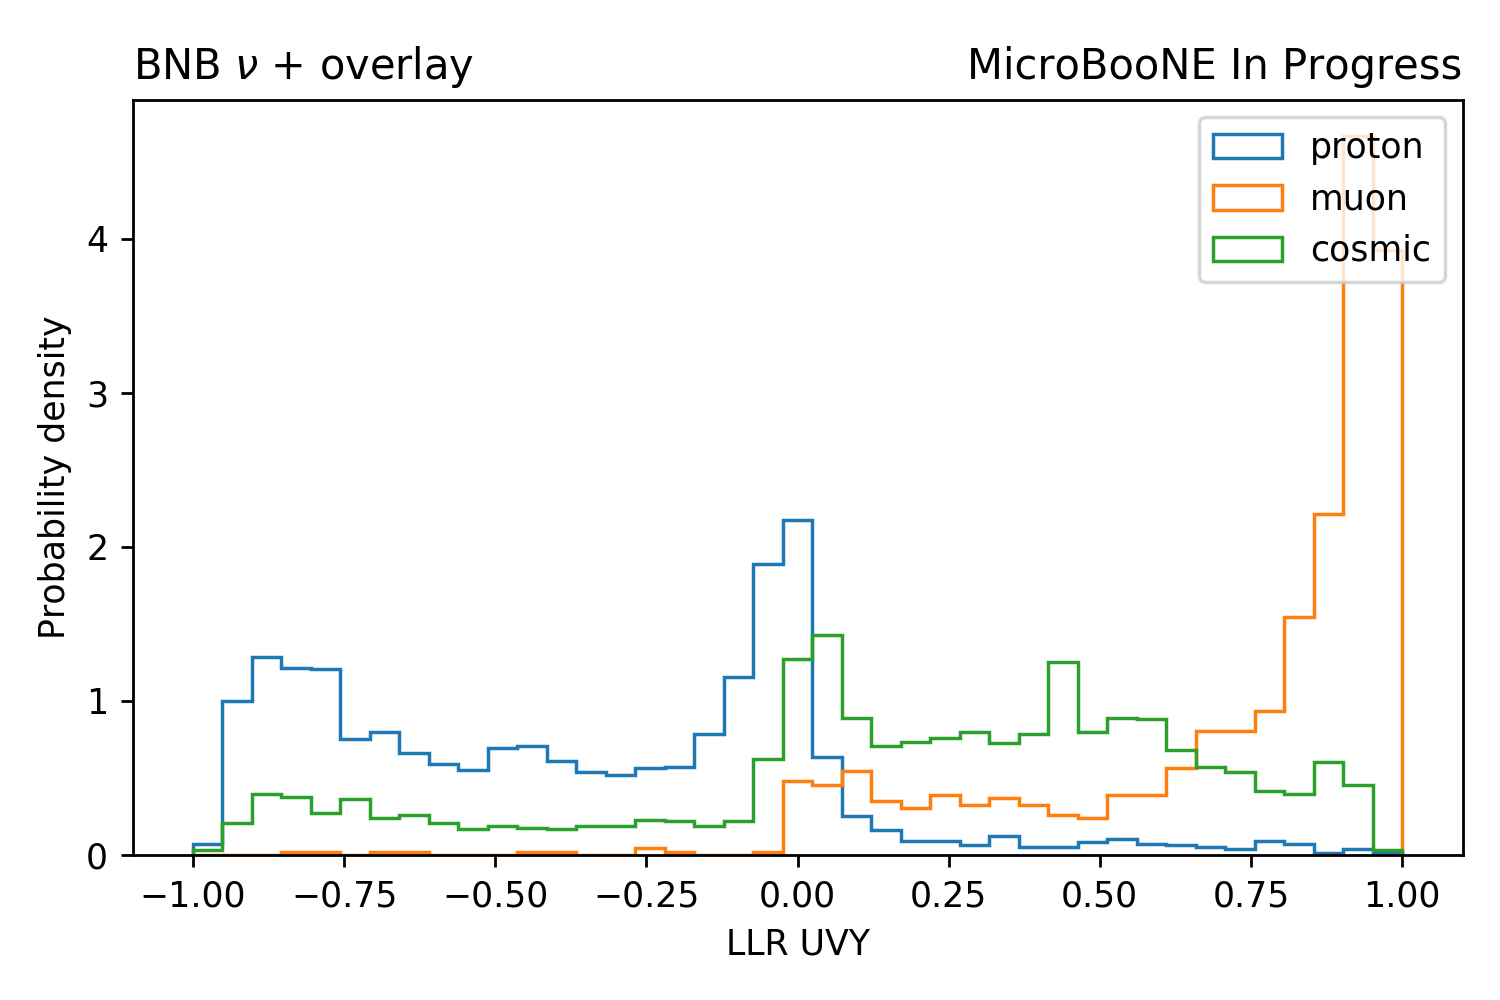
\includegraphics[width=0.7\textwidth]{llrpid/llr_012_n.png}
    \caption{Distribution of the log-likelihood-ratio PID variable for tracks well contained in a fiducial volume, and backtracked to muon (orange), proton (blue), or cosmic (green).}
    \label{fig:llr_pid_uvy_example}
\end{figure}




\subsubsection{$e$/$\gamma$ Separation \textcolor{green}{David, P.R Elena}}
\label{subsec:egammaspearation}
\par Distinguishing electron from photon EM-showers is one of the crucial steps required to perform a measurement of $\nu_e$ interactions in the BNB beam. Photon backgrounds to a $\nu_e$ measurement are largely caused by neutrino interactions with $\pi^0 \rightarrow \gamma\gamma$ in the final state; this topology dominates the $\nu_e$ event rate by approximately an order of magnitude. Three key features distinguish events with $\pi^0$ induced photon showers from $\nu_e$ interactions: (a) the presence of two final state EM showers. (b) the non-zero conversion distance separating the neutrino interaction vertex from the shower start point, and (c) the calorimetric separation via $dE$/$dx$ due to the overlapping ionization segment of $e^+$/$e^-$ pair-conversions through which most $\gamma$ showers manifest themselves. Figure~\ref{fig:egammasep} shows how, at reconstruction level, each of these features can aid in $e$/$\gamma$ separation. This section describes how each of the items above is utilized in the analysis on a technical level, what performance is obtained, and what challenges (both physics- and reconstruction-driven) are encountered when leveraging these variables.

\begin{figure}[ht] 
\begin{center}
    \begin{subfigure}[b]{0.31\textwidth}
    \centering
    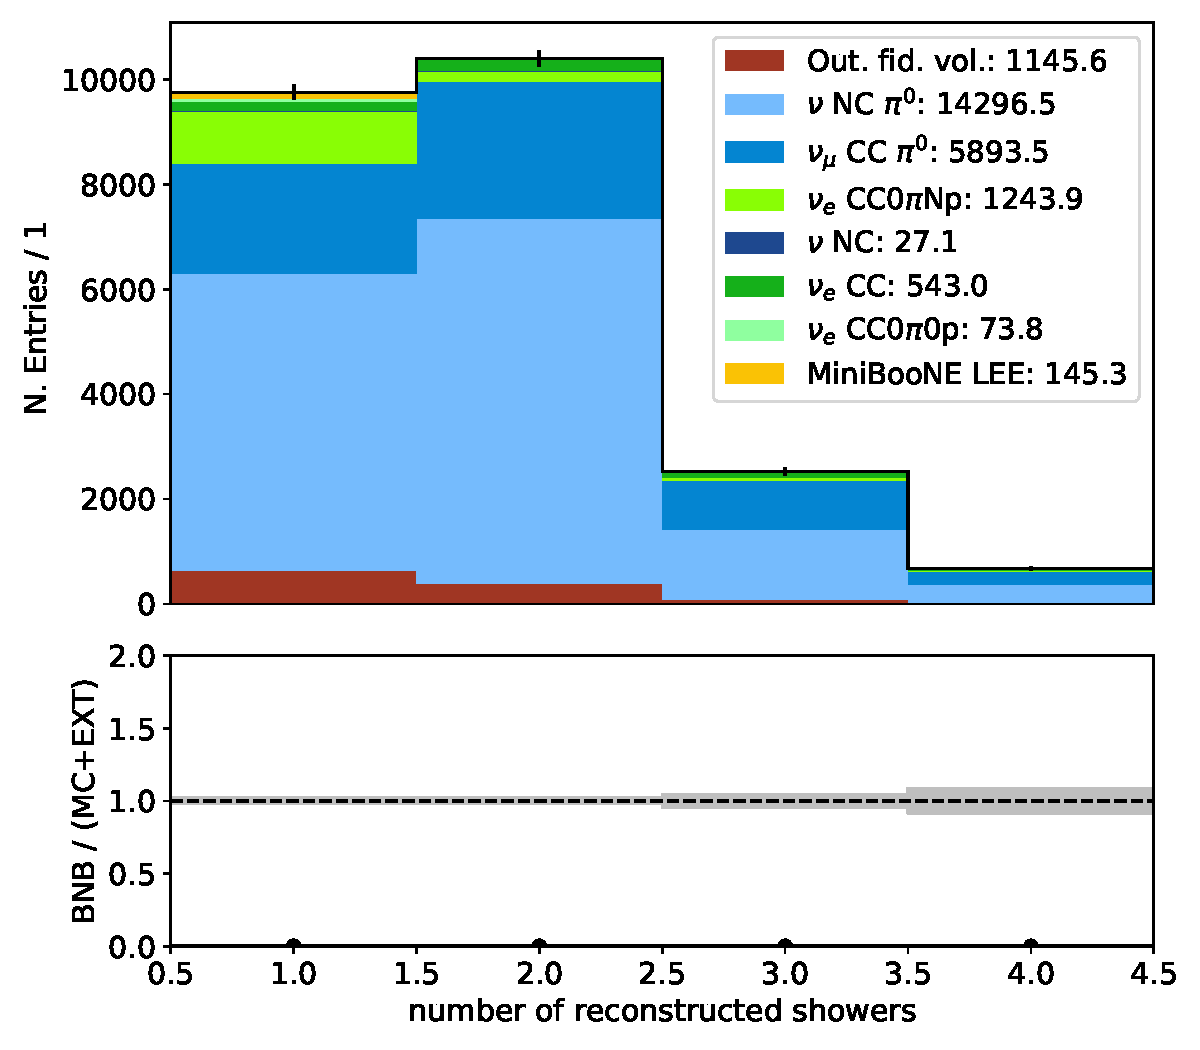
\includegraphics[width=1.00\textwidth]{egamma/n_showers_contained_01022020.pdf}
    \caption{number of reconstructed showers}
    \end{subfigure}
    \begin{subfigure}[b]{0.31\textwidth}
    \centering
    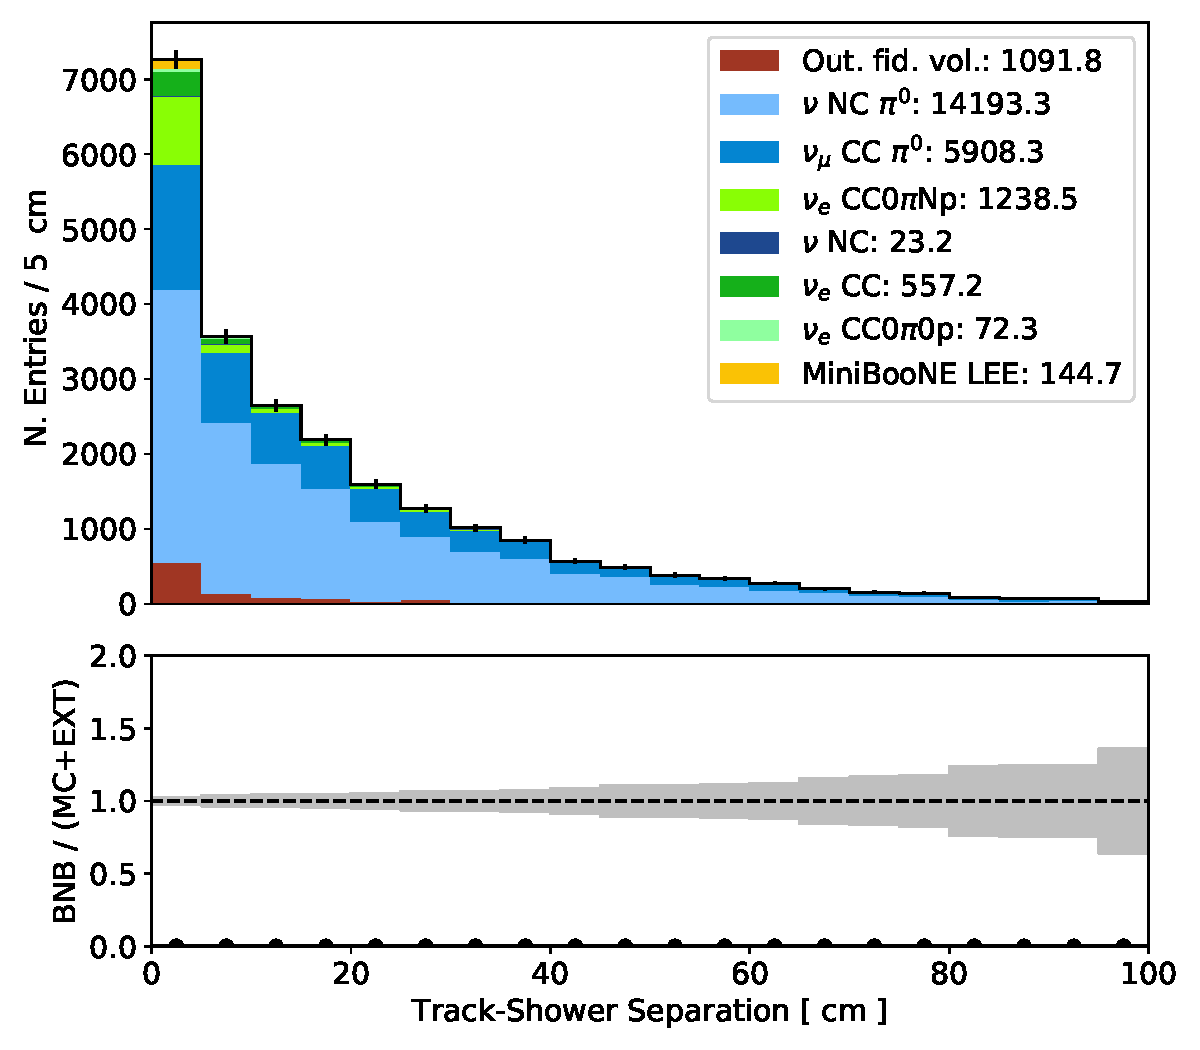
\includegraphics[width=1.00\textwidth]{egamma/tksh_distance_01022020.pdf}
    \caption{track-shower separation}
    \end{subfigure}
    \begin{subfigure}[b]{0.31\textwidth}
    \centering
    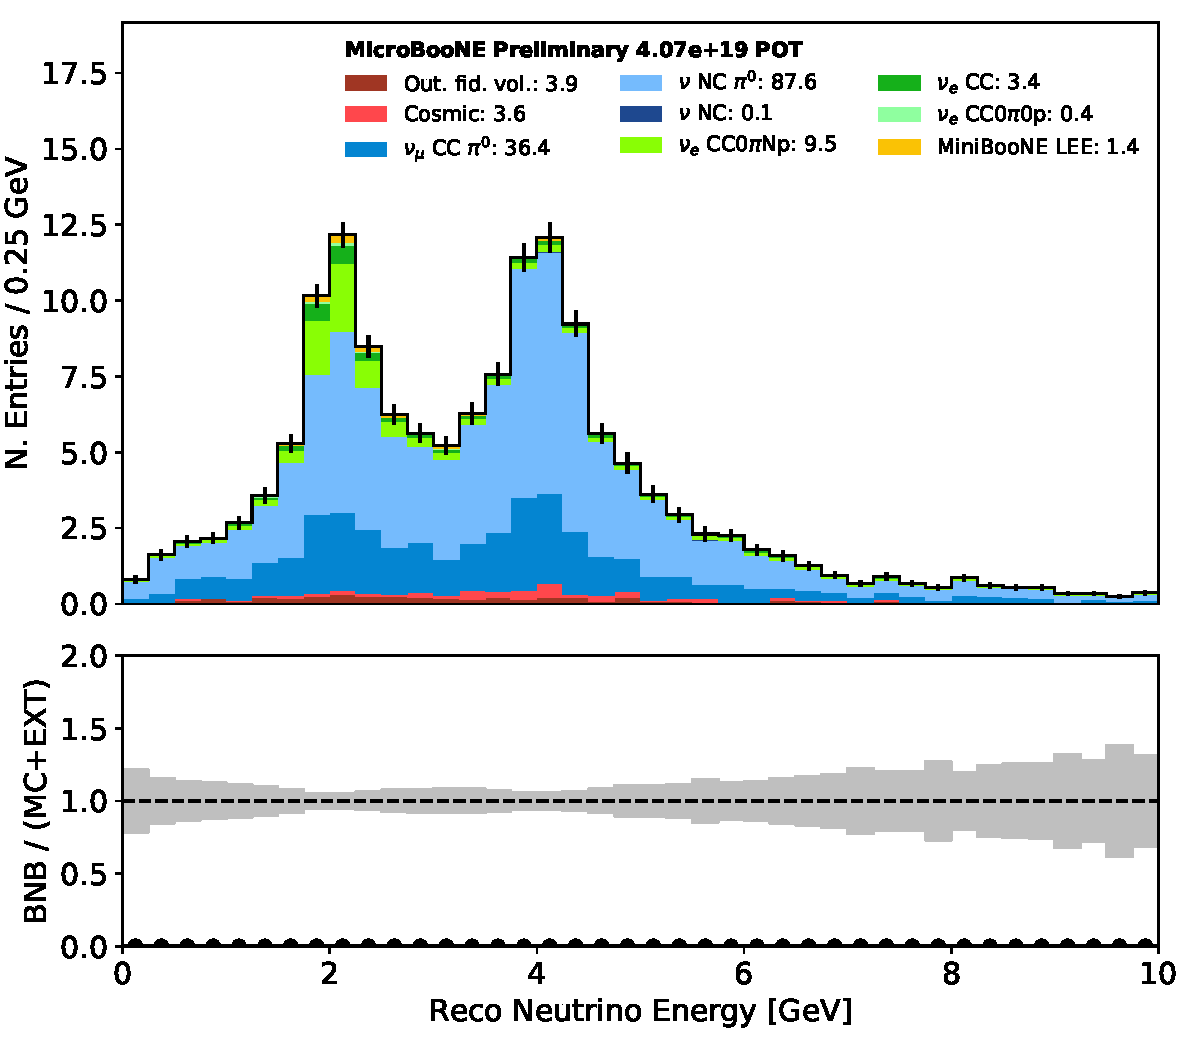
\includegraphics[width=1.00\textwidth]{egamma/shr_tkfit_dedx_Y_01192020.pdf}
    \caption{\label{fig:egammasep:dedx} reconstructed shower $dE$/$dx$}
    \end{subfigure}
\caption{\label{fig:egammasep}Comparison of simulated $\nu_e$ (green) vs. $\nu_{\mu} \rightarrow \pi^0 + X$ (blue) for the three discriminating variables of (a) number of showers, (b) vertex distance, and (c) $dE$/$dx$. Distributions are POT-normalized but contain only $\nu_e$ or $\pi^0$ events (no on/off-beam data distributions).}
\end{center}
\end{figure}

\par \textbf{two-shower requirement} Requiring a single reconstructed shower retains 68\% of $\nu_e$ interactions (with no $\pi^0$ in the final state) while removing 61\% of $\nu_{\mu}$ events with at least one $\pi^0$ in the final state. The fraction of selected $\nu_e$s grows to 79\% when looking below 800 MeV of true energy (the focus of this analysis). Rejection of $\nu_e$s is largely due to events where the electron shower is reconstructed as two separate EM showers, often closely aligned in 3D. Events with final state $\pi^0$s are reconstructed with a single EM shower in the final state because either the second photon escapes the TPC active volume completely (irreducible) or because the second shower is not reconstructed. The dominant causes of this second case are (1) highly-boosted $\pi^0$ decays, in which two aligned photons are merged into one shower and (2) photons which go undetected, often low in energy (below 100 MeV). Additional discriminating variables which aim to recover the reconstruction-related mis-ID of (1) and (2) are utilized in the analysis and presented in Sec.~\ref{sec:nueselection:inputs}.
\par \textbf{track-shower separation} For events where hadronic activity at the neutrino interaction vertex (i.e. final-state protons) is visible, a clear gap between the vertex and the shower start-point can be used to reject $\gamma$ backgrounds. This is a powerful background mitigation tool in the 1$e$N$p$ $\nu_e$ selection. Two factors determine the performance of such a tool: the ability to detect protons and other hadronic activity at the vertex and the accuracy with which the shower start-point is reconstructed. The shower start-point reconstruction accuracy determines the level of background rejection obtainable, as $\gamma$ showers lead to an exponential conversion-distance distribution. \textcolor{blue}{A 1 cm vs. 5 cm track-shower separation cut leads to 95\% vs 74\% mis-ID respectively, but causes a drop in selection efficiency for 1$e$N$p$ events from 72\% to 28\%. I don't think I understand these numbers... because what  I'm understanding is not logical: if I reject events with a 1 cm or more gap, I keep 72\% of nues and 95\% of photons. If I reject events with a 5 cm or more gap, I keep only 28\% nue and 75\% photons. This is completely counter intuitive, what am I getting wrong?  } This is a consequence of the sub-optimal vertex reconstruction accuracy for low-energy $\nu_e$ interactions. In order to enhance the ability to isolate $\nu_e$ events in the 1$e$N$p$ selection through vertex-displacement, different metrics are used to measure the presence of a gap between an electron and proton candidate. These will be described in section~\ref{sec:nueselection:inputs}. It is important to note that this background mitigation strategy is not applicable to single-electron searches, which are an important contribution to $\nu_e$ interactions, especially in the low-energy regime.
\par \textbf{shower d$E$/d$x$} The majority of photons manifest themselves in the TPC through the ionization released by the $e^+$/$e^-$ pair produced via pair-conversion. The electron-positron pair is highly aligned and overlaps on the mm-scale, leading to a doubly-ionizing charge-segment compared to electron showers. To measure this, we use the track fit of the main shower trunk and the calorimetric tools as described in Sec.~\ref{sec:tkshreco}. 
%with a modified version of the MicroBooNE track-fitter~\cite{bib:shrtrackfitter} and for each point along a track the d$Q$/d$x$  and distance from the shower-start are recorded using MicroBooNE's Calorimetry module. This procedure allows to accurately measure d$x$, including small deflections due to the electron's trajectory and SCE offsets, and d$Q$, by incorporating MicroBooNE's full position- and field-dependent relative and absolute charge calibration. From d$Q$/d$x$, d$E$/d$x$ is calculated assuming a fixed recombination correction assuming 2.1 MeV/cm energy loss, but accounting for local variations in the electric field. 
The distinctive 4 MeV/cm population expected for $\gamma$ showers is visible in figure~\ref{fig:egammasep:dedx}. The main limitation to $e$/$\gamma$ separation via d$E$/d$x$ is the large fraction of photons reconstructed with a d$E$/d$x$ of less then 3 MeV/cm (23\% of $\pi^0$ events fall in the 1-3 MeV range). This is due both to mis-reconstructed events, for which the start-point is incorrectly reconstructed by more than one or two cm, and to events where the photon shower's energy loss-profile is not as clearly distinguishable from that of a single electron. While the relative contribution of these two sources is still under determination, the second causes a significant mis-ID rate, and is largely associated to lower-energy $\gamma$ showers for which the production of a highly asymmetric electron-positron pair where one of the electrons is barely visible is more frequent. The impact of shower energy on the measured d$E$/d$x$ for a $\gamma$ shower is shown in figure~\ref{fig:dedxgammas:energy}. Below 100 MeV, where most $\gamma$ showers in the BNB are produced, the reconstructed d$E$/d$x$ is electron-like. The impact of distance from the shower start-point on whether d$E$/d$x$ is reconstructed to be 2 or 4 MeV/cm is also important, as can be seen in figure~\ref{fig:dedxgammas:dist}. This is particularly true for low-energy asymmetric pair-production events, and motivates utilizing 
d$E$/d$x$ information at different distances from the shower start-point for $e$/$\gamma$ separation.
\begin{figure}[H] 
\begin{center}
    \begin{subfigure}[b]{0.45\textwidth}
    \centering
    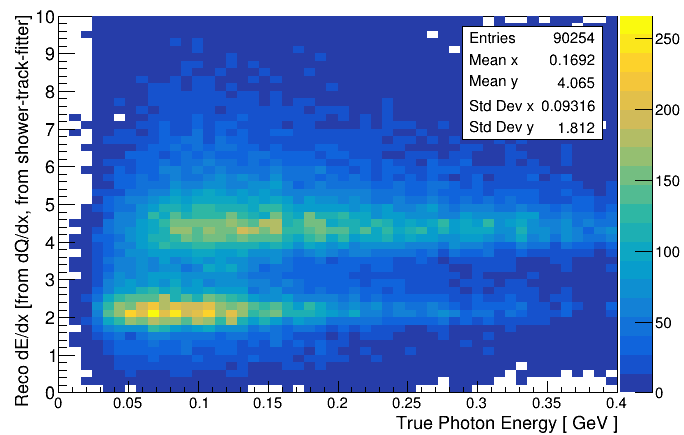
\includegraphics[width=1.00\textwidth]{egamma/dedx_vs_energy_gamma.png}
    \caption{\label{fig:dedxgammas:energy} d$E$/d$x$ vs. distance from shower start-point for $\gamma$ showers \textcolor{blue}{wrong caption}}
    \end{subfigure}
    \begin{subfigure}[b]{0.45\textwidth}
    \centering
    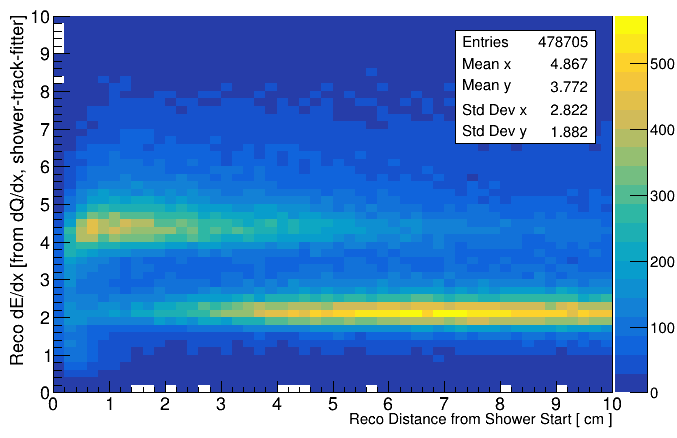
\includegraphics[width=1.00\textwidth]{egamma/dedx_vs_dist_gamma.png}
    \caption{\label{fig:dedxgammas:dist} d$E$/d$x$ vs. distance from shower start-point for $\gamma$ showers}
    \end{subfigure}
\caption{\label{fig:dedxgammas}}
\end{center}
\end{figure}



%\newpage

\subsection{Energy Reconstruction \textcolor{green}{Giuseppe + David... (PR Elena)}}
\label{sec:ereco}
\par Energy reconstruction is performed thought calorimetry for EM showers and through a measurement of a track's range for contained muons and protons. For \textcolor{blue}{should we add "uncontained"} muons, multiple Coulomb scattering (MCS) is also used to estimate the muon energy. The energy resolution obtained for different particles is reported in table~\ref{tab:eres}. More information on each particle's energy resolution is reported in figure~\ref{fig:eres:particle} where the 2D reconstructed vs. true energy distribution (in log-scale) is shown on the left, next to a plot of energy resolution vs. true energy on the right. The energy resolution reported here is obtained from a Gaussian plus one-sided exponential fit to the distribution $[E_{\rm reco}-E_{\rm true}] / E_{\rm true}$, see figures \ref{fig:eres:elec:binned}. The resolution reported refers only to the Gaussian width $\sigma$ extracted in the fit, and therefore does not account for negative tails, which are significant in the case of EM shower energy reconstruction, and described below.


\begin{table}[H]
\centering
  \begin{tabular}{ | c | c |  }
    \hline
    particle & kinetic energy resolution  \\ \hline
    proton & 4\% at 100 MeV 1\% at 200 MeV \\ \hline
    muon (range) & 3\%  \\ \hline
    muon (MCS) & $\frac{4.7\%}{\sqrt{E/{\rm GeV}}} \otimes \frac{2.8\%}{E/{\rm GeV}} \otimes 0.0\% \text{\textcolor{blue}{this is fairly confusing, especially the 0.0\%, can we add a reference, or an explaination?}}$  \\ \hline
    electron & 15\%  \\
    \hline
    
  \end{tabular}
  \caption{\label{tab:eres} Energy resolution for different particle species.}
 \end{table}
 
 \par For EM showers, the calorimetric energy reconstruction response has a significant non-Gaussian component, as well as a large bias. Both effects are attributable to reconstruction effects associated with under-clustering of charge. The energy bias is found to be 20\% and approximately flat in energy, and motivates a definition of a corrected shower energy, defined as $E_{\rm corrected} = E_{\rm calorimetry} / 0.8$. The non-Gaussian response for EM energy reconstruction can be modeled through a Gaussian plus one-sided exponential distribution. Figure~\ref{fig:eres:elec:binned} shows in different bins of true energy the fractional energy response and a fit to a Gaussian plus one-sided exponential function. The residual energy bias, after the 20\% correction applied, is of order $3-8$\%. 
 
\begin{figure}[ht]
\begin{center}
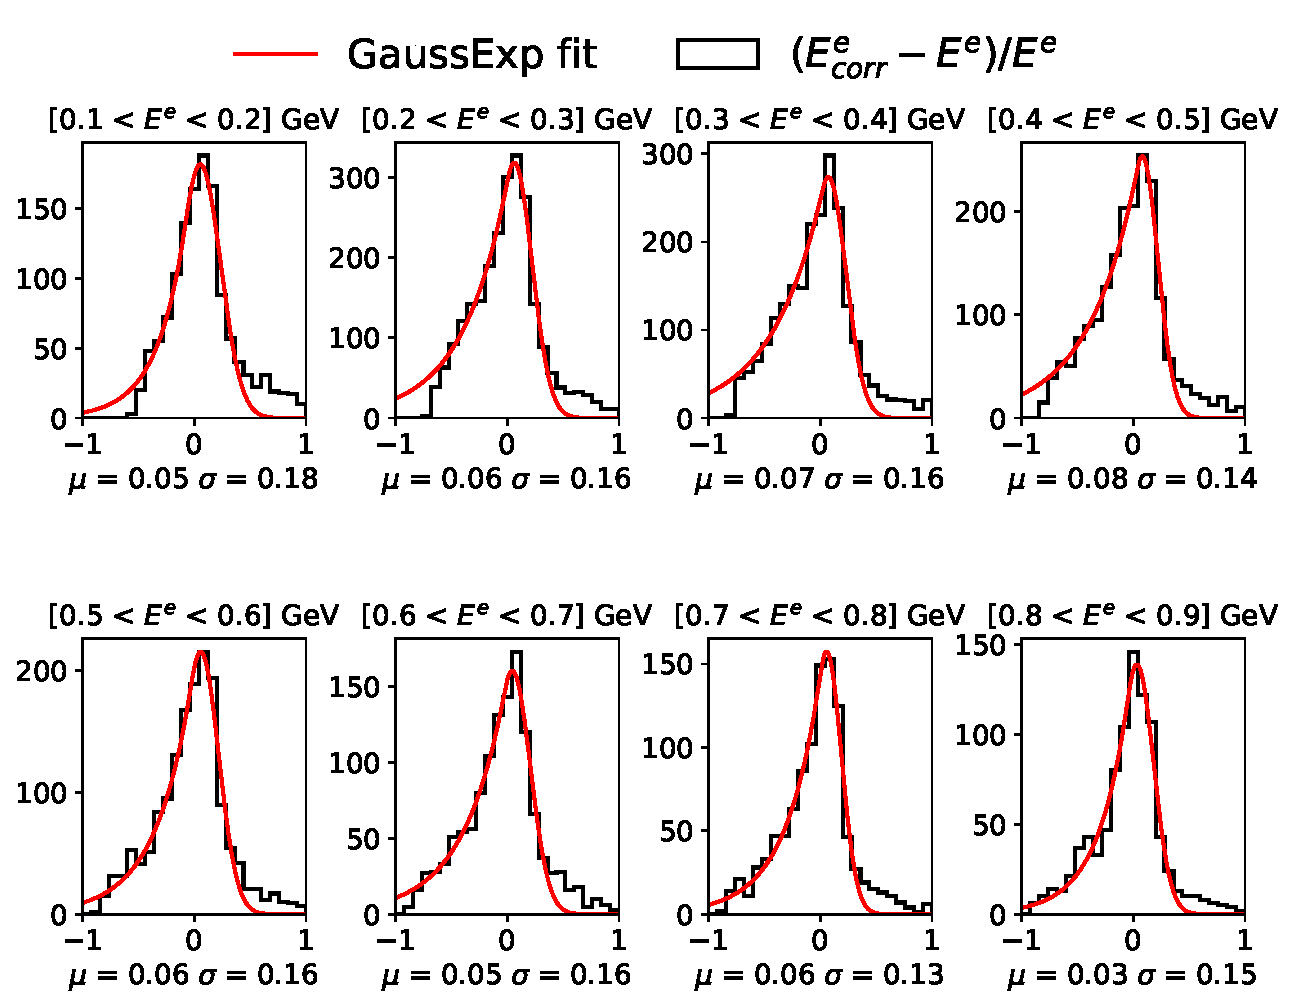
\includegraphics[width=0.75\textwidth]{ereco/elec_eres_binned.pdf}
\caption{\label{fig:eres:elec:binned}Energy resolution for electron showers.}
\end{center}
\end{figure}
 
\clearpage

\begin{figure}[H] 
\begin{center}
    \begin{subfigure}[b]{0.4\textwidth}
    \centering
    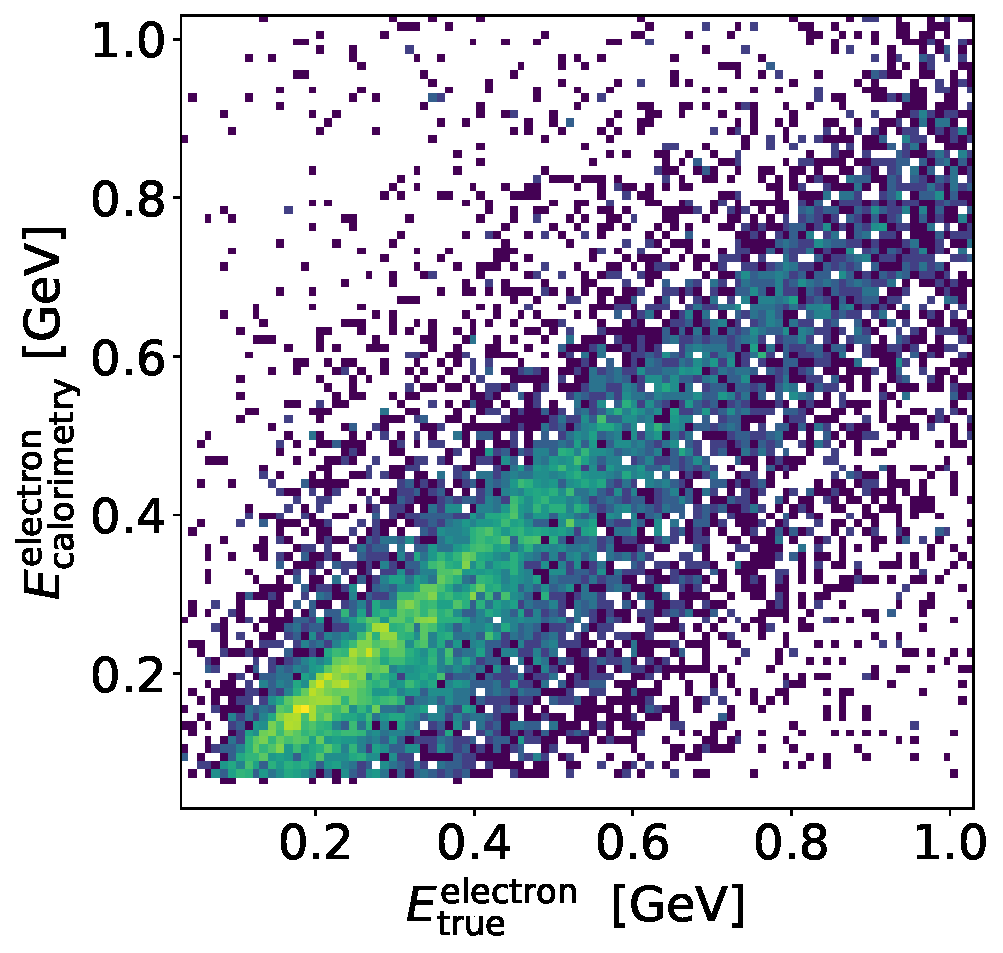
\includegraphics[width=1.00\textwidth]{ereco/electron_eres2D.pdf}
    %\caption{\label{fig:eres:elec:2d} }
    \end{subfigure}
    \begin{subfigure}[b]{0.38\textwidth}
    \centering
    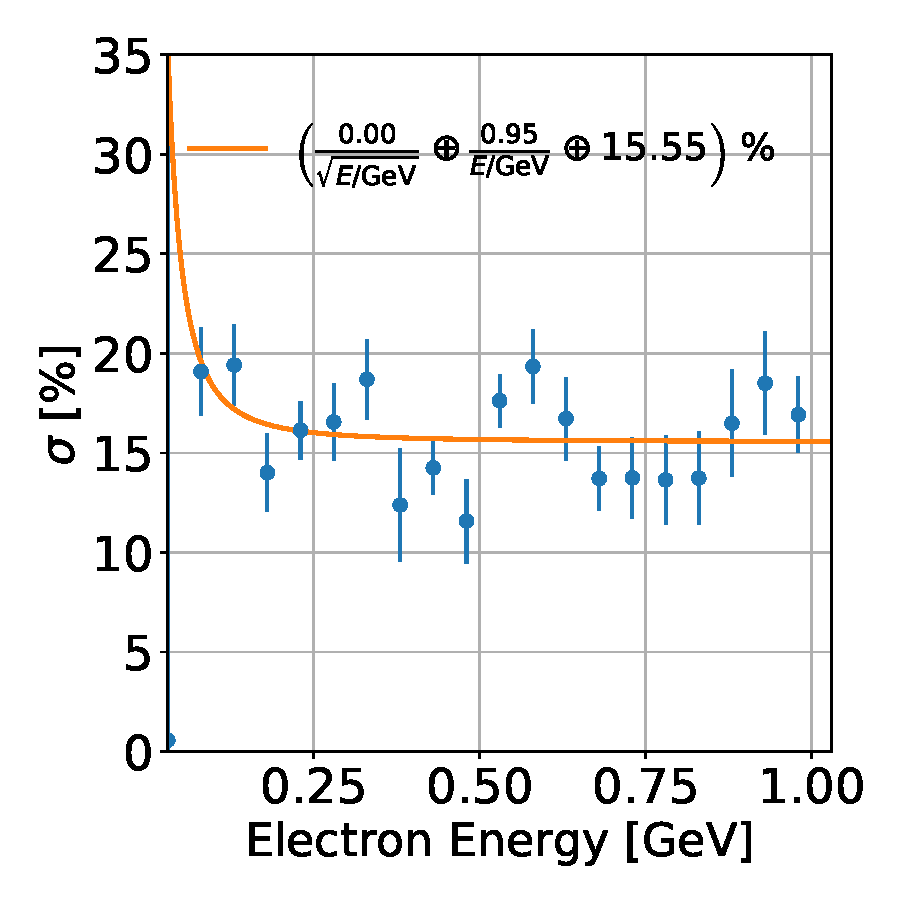
\includegraphics[width=1.00\textwidth]{ereco/elec_eres_vs_true.pdf}
    %\caption{\label{fig:eres:elec:vstrue} }
    \end{subfigure}
    \begin{subfigure}[b]{0.4\textwidth}
    \centering
    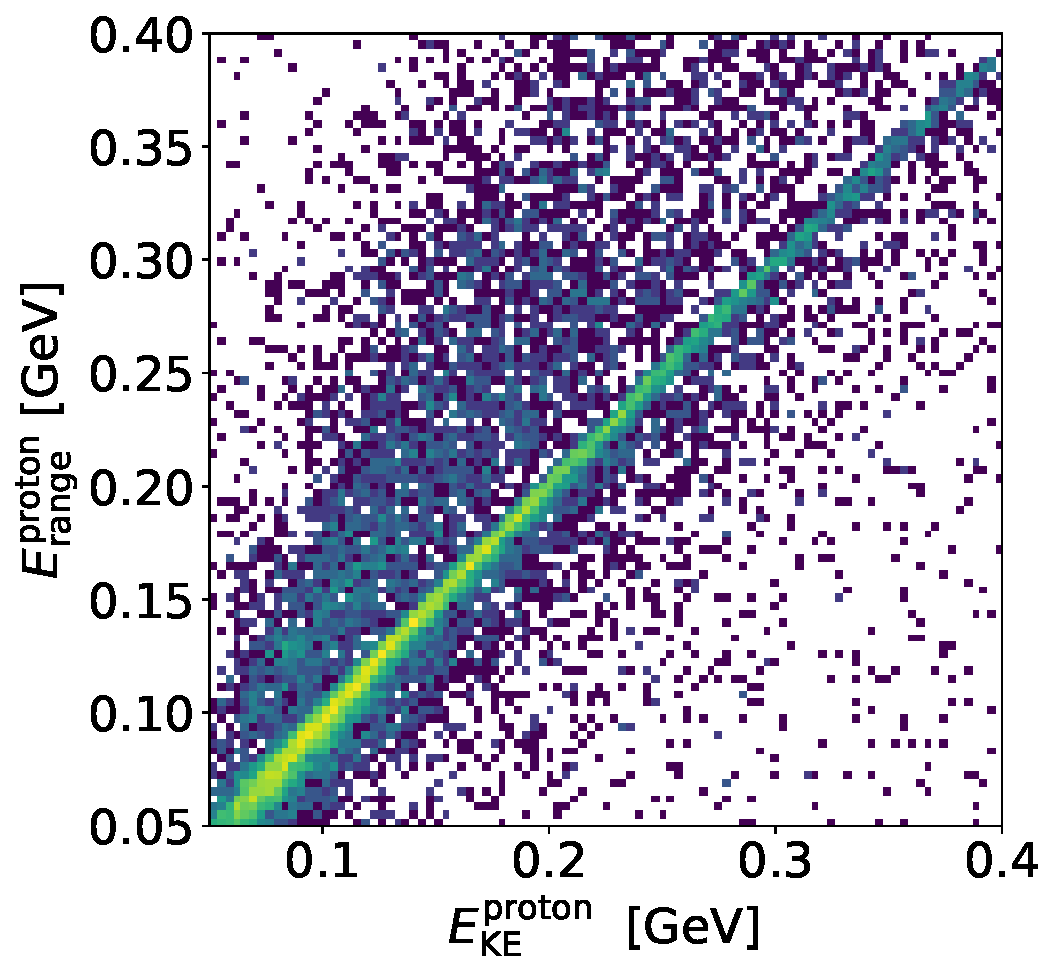
\includegraphics[width=1.00\textwidth]{ereco/proton_eres2D.pdf}
    %\caption{\label{fig:eres:proton:2d} }
    \end{subfigure}
    \begin{subfigure}[b]{0.38\textwidth}
    \centering
    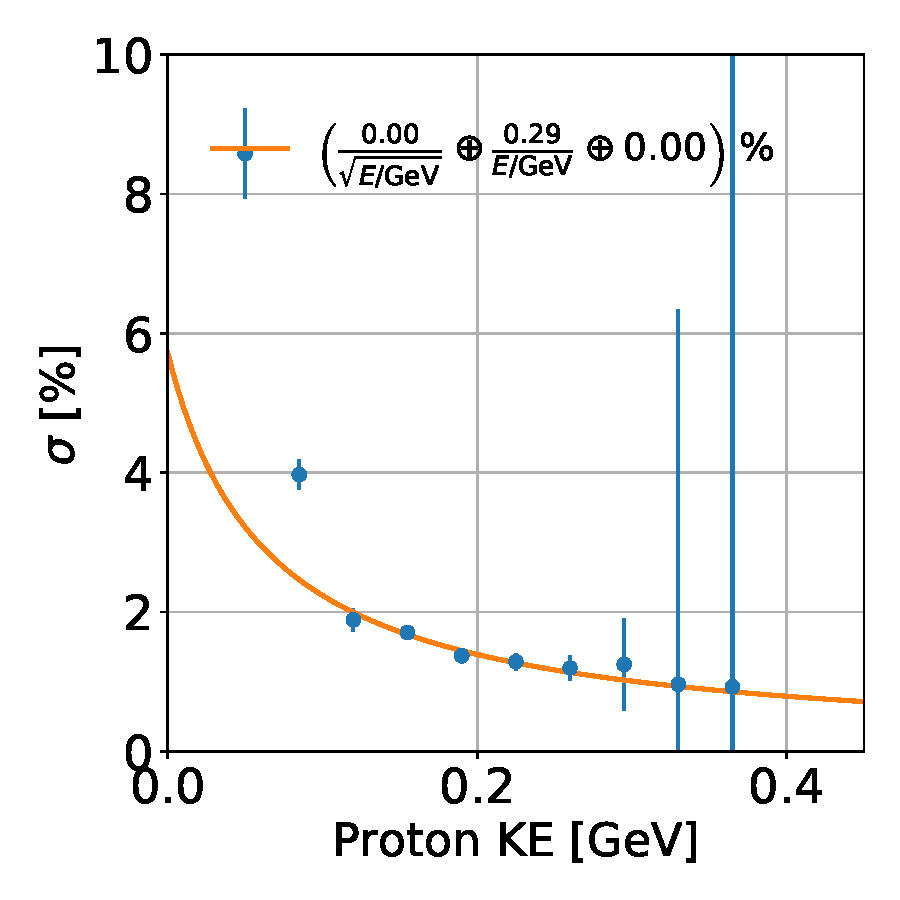
\includegraphics[width=1.00\textwidth]{ereco/proton_eres_vs_true.pdf}
    %\caption{\label{fig:eres:proton:vstrue} }
    \end{subfigure}
    \begin{subfigure}[b]{0.4\textwidth}
    \centering
    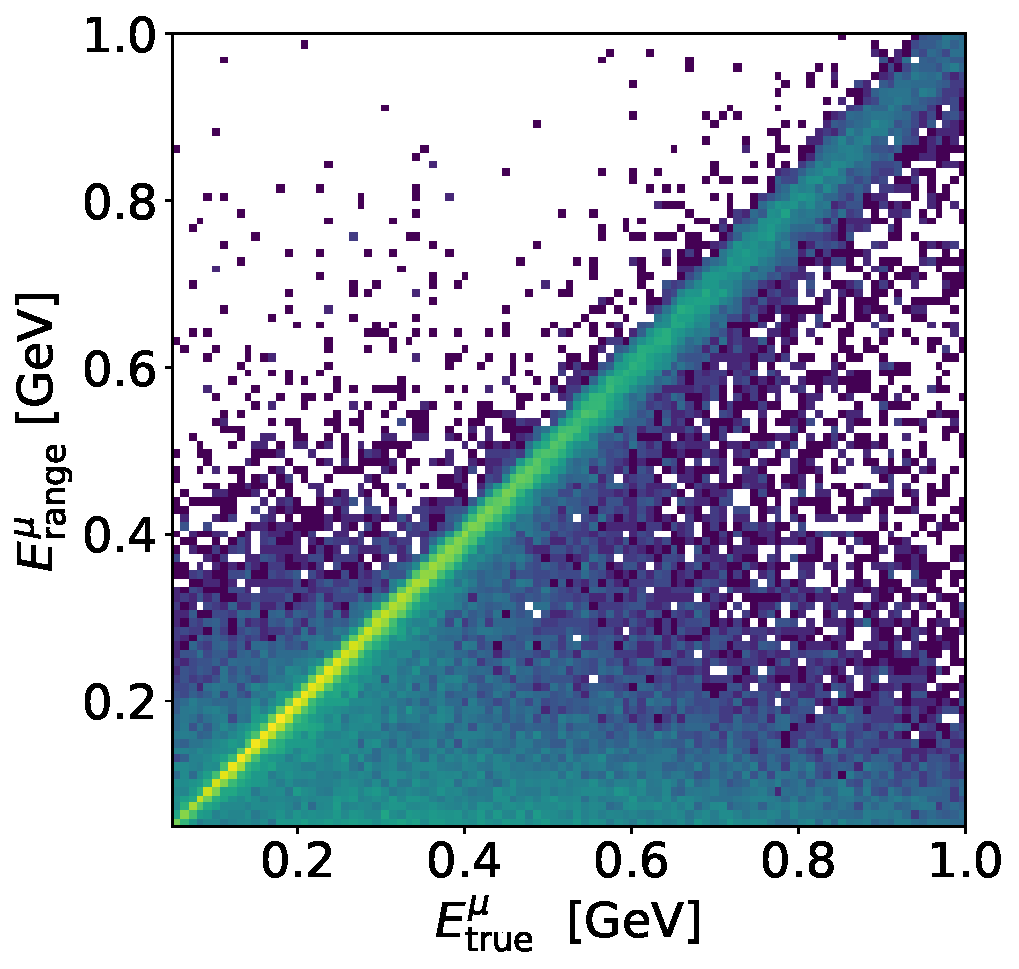
\includegraphics[width=1.00\textwidth]{ereco/muon_range_eres2D.pdf}
    %\caption{\label{fig:eres:muon:2d} }
    \end{subfigure}
    \begin{subfigure}[b]{0.38\textwidth}
    \centering
    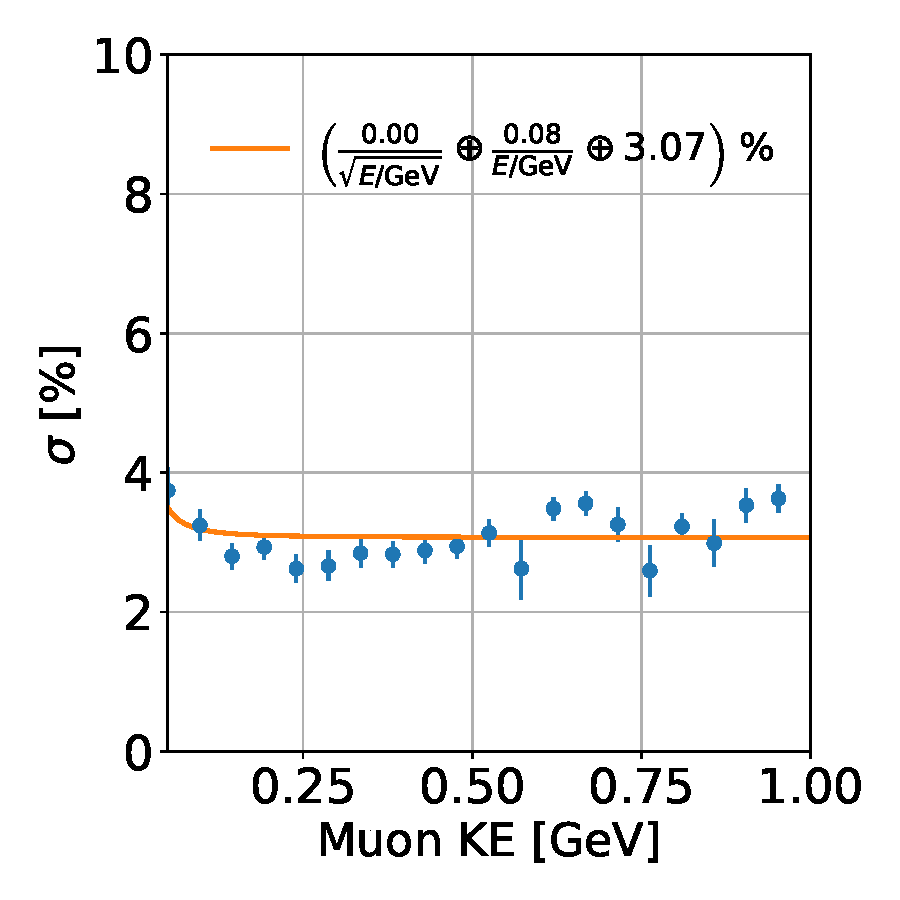
\includegraphics[width=1.00\textwidth]{ereco/muon_range_eres_vs_true.pdf}
    %\caption{\label{fig:eres:muon:vstrue} }
    \end{subfigure}
\caption{\label{fig:eres:particle}Energy resolution for electrons (top), protons (center) and muons (bottom). Left: reconstructed vs. true energy resolution (log-scale). Right: energy resolution from Gaussian fit to $[E_{\rm reco}-E_{\rm true}] / E_{\rm true}$.}
\end{center}
\end{figure}

\subsubsection{Neutrino Energy Reconstruction \textcolor{green}{Giuseppe + David, P.R. Elena}}

\par In this analysis, the energy reconstruction for neutrino interactions is performed through a sum of the visible energy of the various reconstructed final-state particles in the interaction. For $\nu_e$ events, the reconstructed energy is defined as:
\begin{equation}
    E_{\rm reco}^{\nu_e} = E_{\rm corrected}^{\rm electron} + \sum_{\rm tracks} E_{\rm range}^{\rm proton}.
\end{equation}{}
\textcolor{blue}{is this true also for nue inclusive?}.
For contained $\nu_{\mu}$ interactions, the reconstructed energy is defined as:

\begin{equation}
    E_{\rm reco}^{\nu_{\mu}} = E_{\rm range}^{\rm muon} + \sum_{\rm protons} E_{\rm range}^{\rm proton} + 0.105 \; GeV
\end{equation}{}

Figure~\ref{fig:eres:neutrino} shows the comparison between reconstructed energy and truth visible energy, which is defined as the sum of the lepton energy, pion energy (if present), and proton energy (for all protons above 40 MeV of KE). This comparison shows very accurate energy reconstruction for $\nu_{\mu}$ events \textcolor{blue}{uhm.... this is true up to a point: there's a tail for high numu visible and log numu range: does this come from events w/ non-contained muons?}. For $\nu_e$ interactions, with smearing dominated by the worse energy resolution of electron showers \textcolor{blue}{This sentence misses a verb}.

\begin{figure}[H] 
\begin{center}
    \begin{subfigure}[b]{0.4\textwidth}
    \centering
    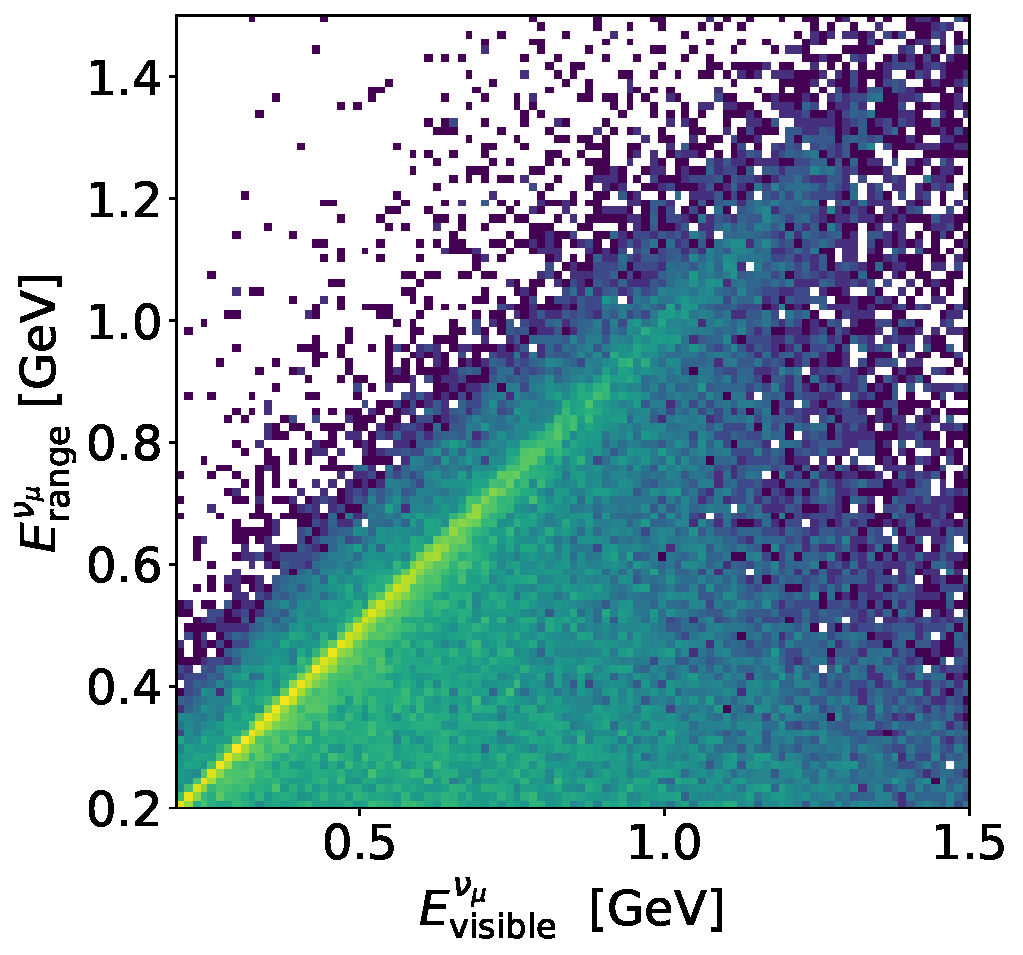
\includegraphics[width=1.00\textwidth]{ereco/numu_energy_visible_eres2D.pdf}
    \caption{\label{fig:eres:numu:2d} }
    \end{subfigure}
    \begin{subfigure}[b]{0.4\textwidth}
    \centering
    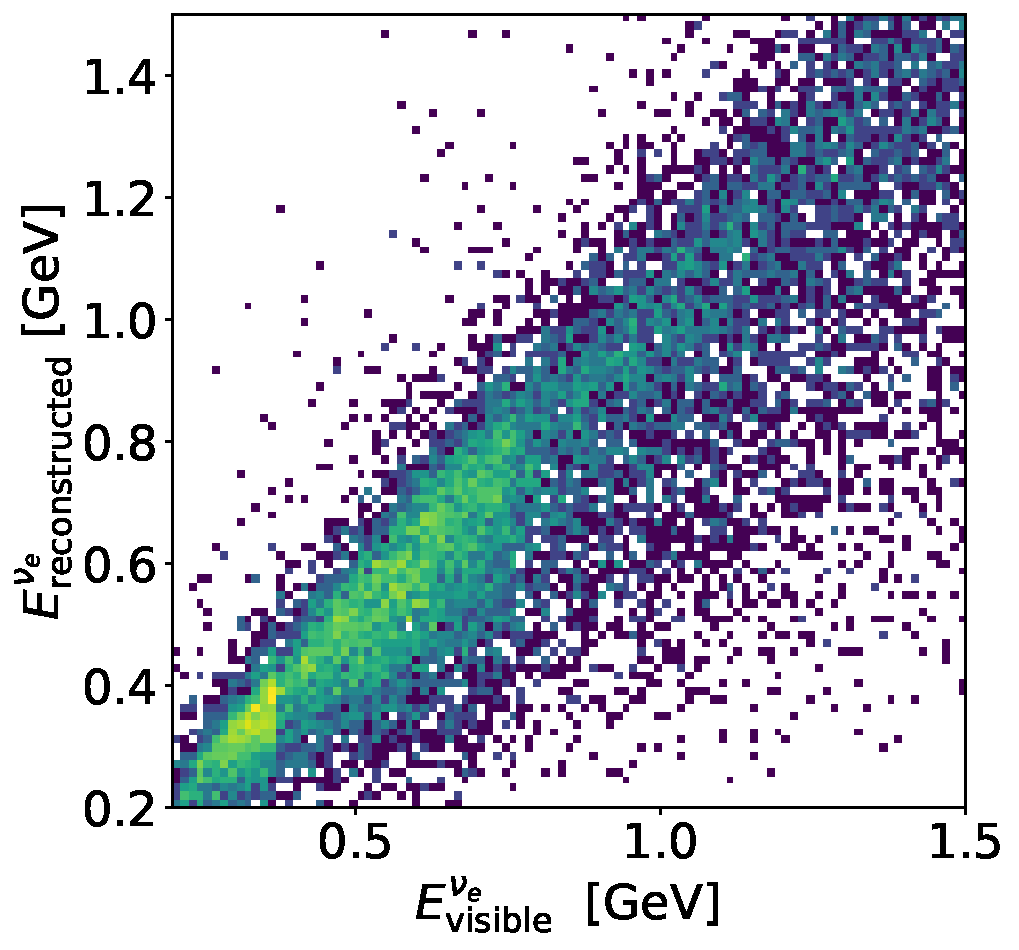
\includegraphics[width=1.00\textwidth]{ereco/nue_visible_eres2D.pdf}
    \caption{\label{fig:eres:nue:vstrue} }
    \end{subfigure}
\caption{\label{fig:eres:neutrino}Log-scale color-maps.}
\end{center}
\end{figure}

\newpage

\section{Control Samples and Analysis Input Validation}
\label{sec:controls}

\par The selections and analysis described below rely on well understood detector, simulation, calibration, and analysis tools performance. This section is dedicated to evaluating the performance of detector modeling through data-mc comparisons of targeted samples. The sidebands developed for this analysis are a high-stats $\pi^0$ selection, and an \emph{anti-BDT} filter which targets the selection of $\nu_e$ like backgrounds. \emph{Currently comparisons for the \emph{anti-BDT} filter are not available and will be documented in a future iteration of this note.}
\par It is important to note that in addition to detector simulation and reconstruction effects, $\nu$-Ar modeling can impact the level of data-mc agreement in various variables. We will try to point out when this might be the case.
\subsection{$\pi^0$ control sample}
\label{sec:controls:pi0}
\par A $\pi^0$ selection has been developed in order to obtain high-stats samples of $\pi^0$ events and $\gamma$ EM showers which can constrain $\pi^0$ production modeling uncertainties as well as validate the analyis' ability to reconstruct and select EM showers.
\par Figure~\ref{fig:pi0:mass} shows the reconstructed di-photon mass (\texttt{M$\gamma\gamma$}) for candidate $\pi^0$ events, with a calibrated but uncorrected \footnote{With the term ``uncorrected", we mean that we do not account for biases in shower energy reconstruction caused by the incompleteness in charge clustering.} energy reconstruction. Overall, there is good data-MC agreement in shape, apart from an apparent normalization difference. To account for this normalization difference, we measure the flat scaling factor  for CC and NC $\pi^0$ events needed to obtain  a consistent rate in data and MC: this factor is 72.4\% in Run1 and 72.7\% in Run3. We repeat the exercise applying a tighter $\pi^0$ selection enhancing the $\pi^0$ purity and obtain scaling factors of 70\% for both Run1 and Run3. While this procedure is far from rigorous, it allows us to study detector-related and specifically shower-related variables removing a large normalization difference. \emph{A more rigorous data-driven constrain of our $\pi^0$ rate, performed accounting for detector and flux systematics, and considering a broader range of $\pi^0$ modeling, will need to be performed.}

\begin{figure}[H] 
\begin{center}
    \begin{subfigure}[b]{0.3\textwidth}
    \centering
    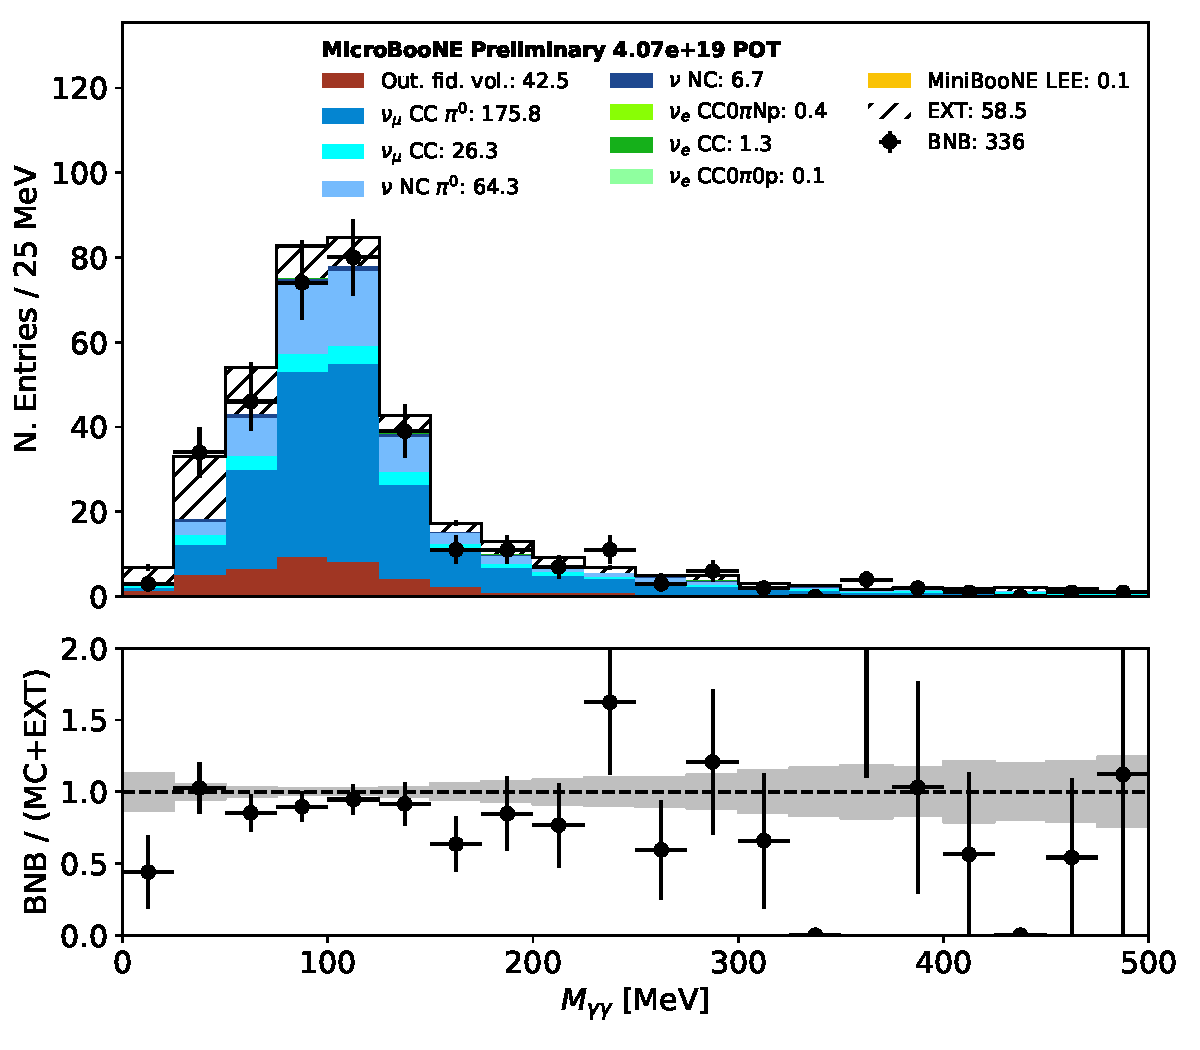
\includegraphics[width=1.00\textwidth]{pi0/pi0_mass_Y_01142020_5E19.pdf}
    \caption{\label{fig:pi0:mass:5E19} Run 1 ``5E19'' open dataset.}
    \end{subfigure}
    \begin{subfigure}[b]{0.3\textwidth}
    \centering
    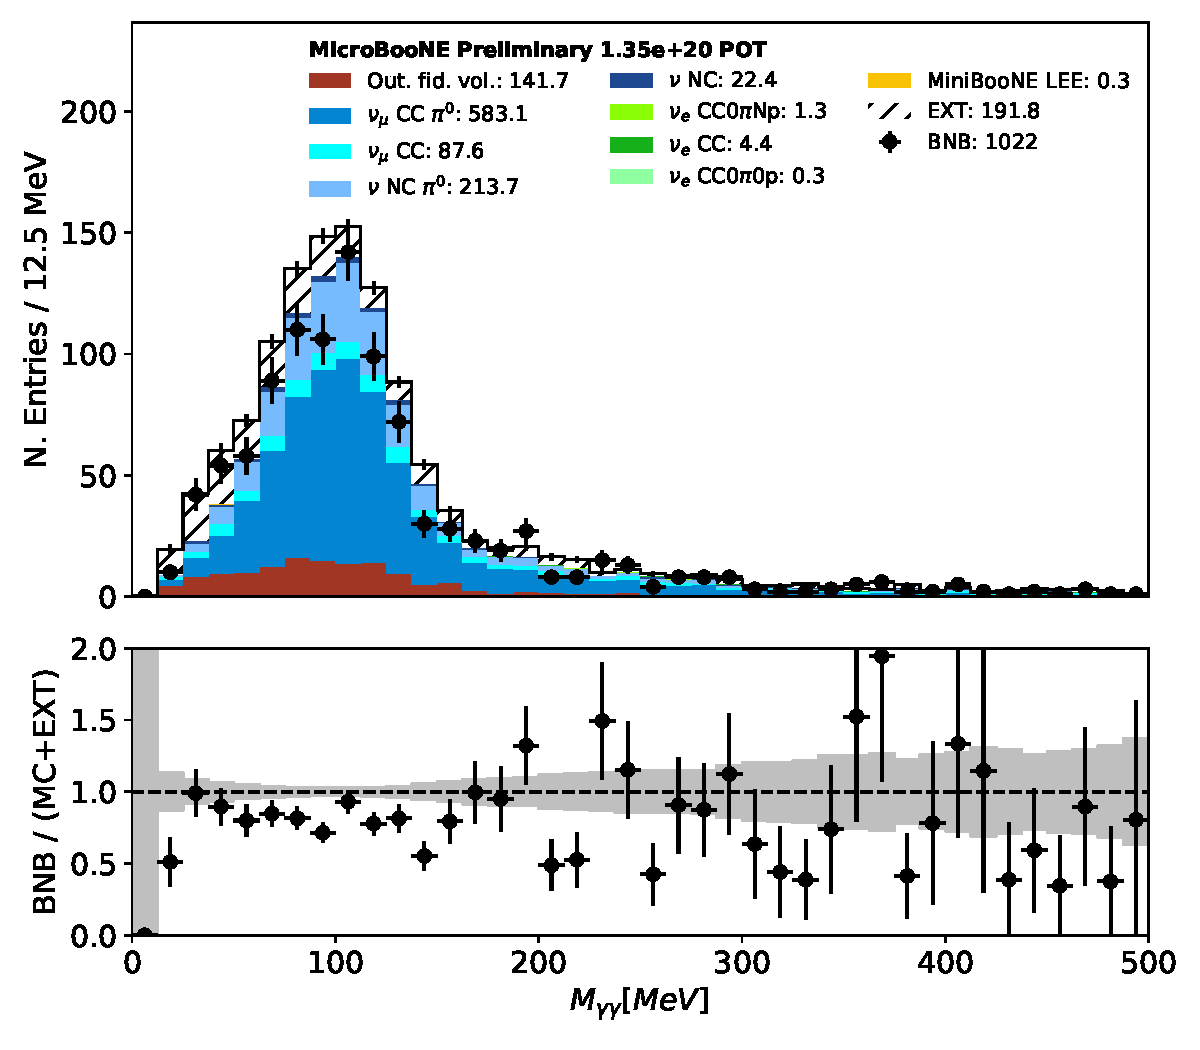
\includegraphics[width=1.00\textwidth]{pi0/pi0_mass_Y_01142020sel__RUN1.pdf}
    \caption{\label{fig:pi0:mass:5E19} Run 1.}
    \end{subfigure}
    \begin{subfigure}[b]{0.3\textwidth}
    \centering
    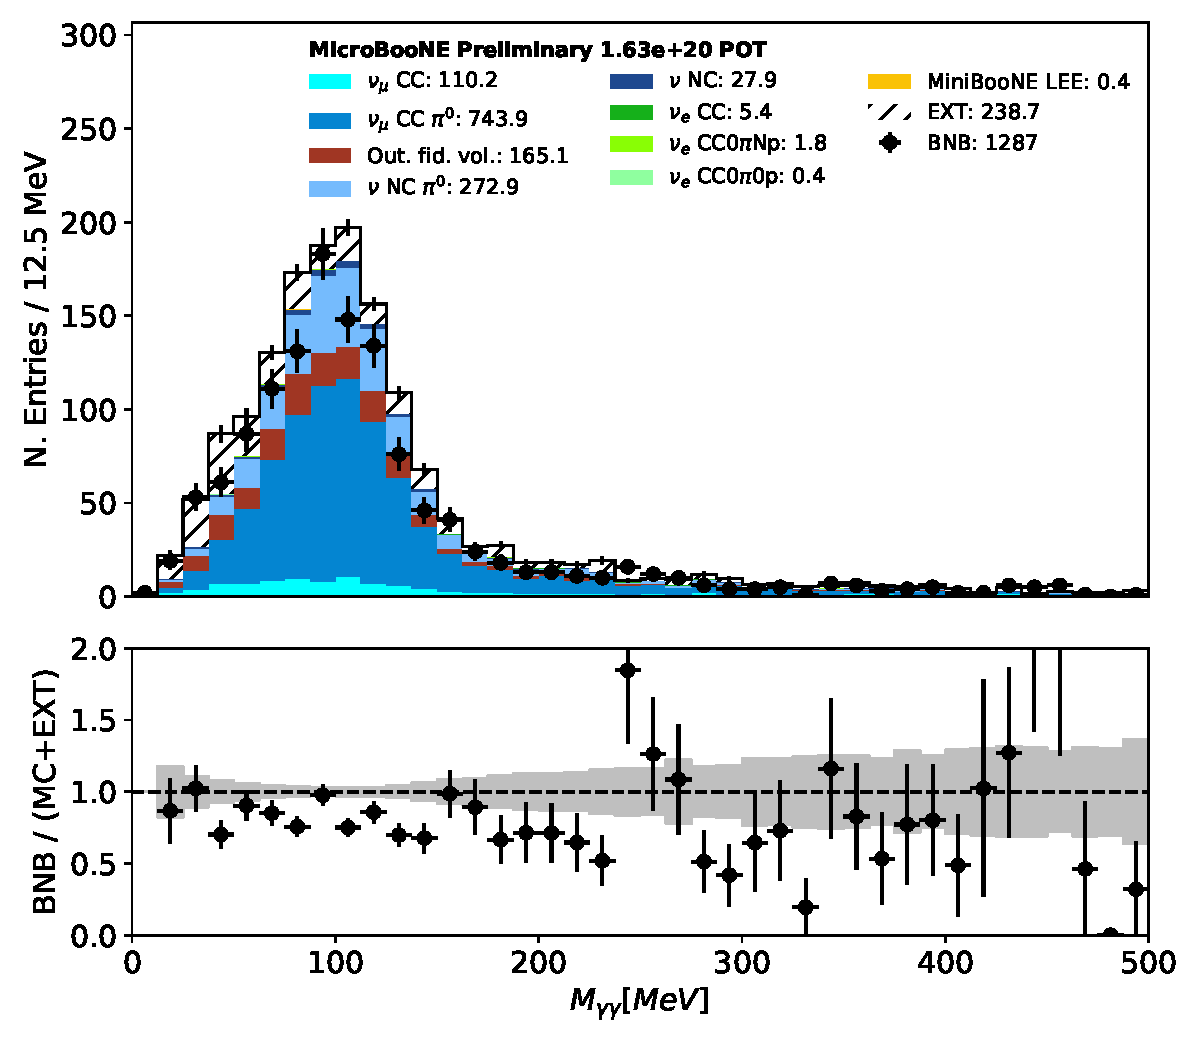
\includegraphics[width=1.00\textwidth]{pi0/pi0_mass_Y_01142020sel_RUN3.pdf}
    \caption{\label{fig:pi0:mass:5E19} Run 3.}
    \end{subfigure}
\caption{\label{fig:pi0:mass}Reconstructed $\pi^0$ mass.}
\end{center}
\end{figure}

\par After applying a scaling factor of 0.7 to CC and NC $\pi^0$ events in the MC, we show comparisons of shower variables with the goal of assessing data-mc agreement for the $\nu_e$ selection. Figure~\ref{fig:pi0:datamc} shows reconstructed quantities used in the $\nu_e$ analysis for $\pi^0$ candidate events which are useful in validating the robustness of shower modeling. They include leading and sub-leading shower dE/dx (top), followed by the leading and sub-leading shower conversion distance and shower score. The last row reports the reconstructed shower Moliere angle and track PID score for the longest track in each event. Generally, the data-MC agreement is quite good. For d$E$/d$x$ there appears to be a one bin shift to the left in data, specifically in the 4 MeV/cm peak associated with photons (see figure~\ref{fig:pi0:datamc} top-left). \emph{A re-calibration of shower d$E$/d$x$ is planned for the analysis, but has not been fully implemented at the moment.}

\begin{figure}[H] 
\begin{center}
    \begin{subfigure}[b]{0.38\textwidth}
    \centering
    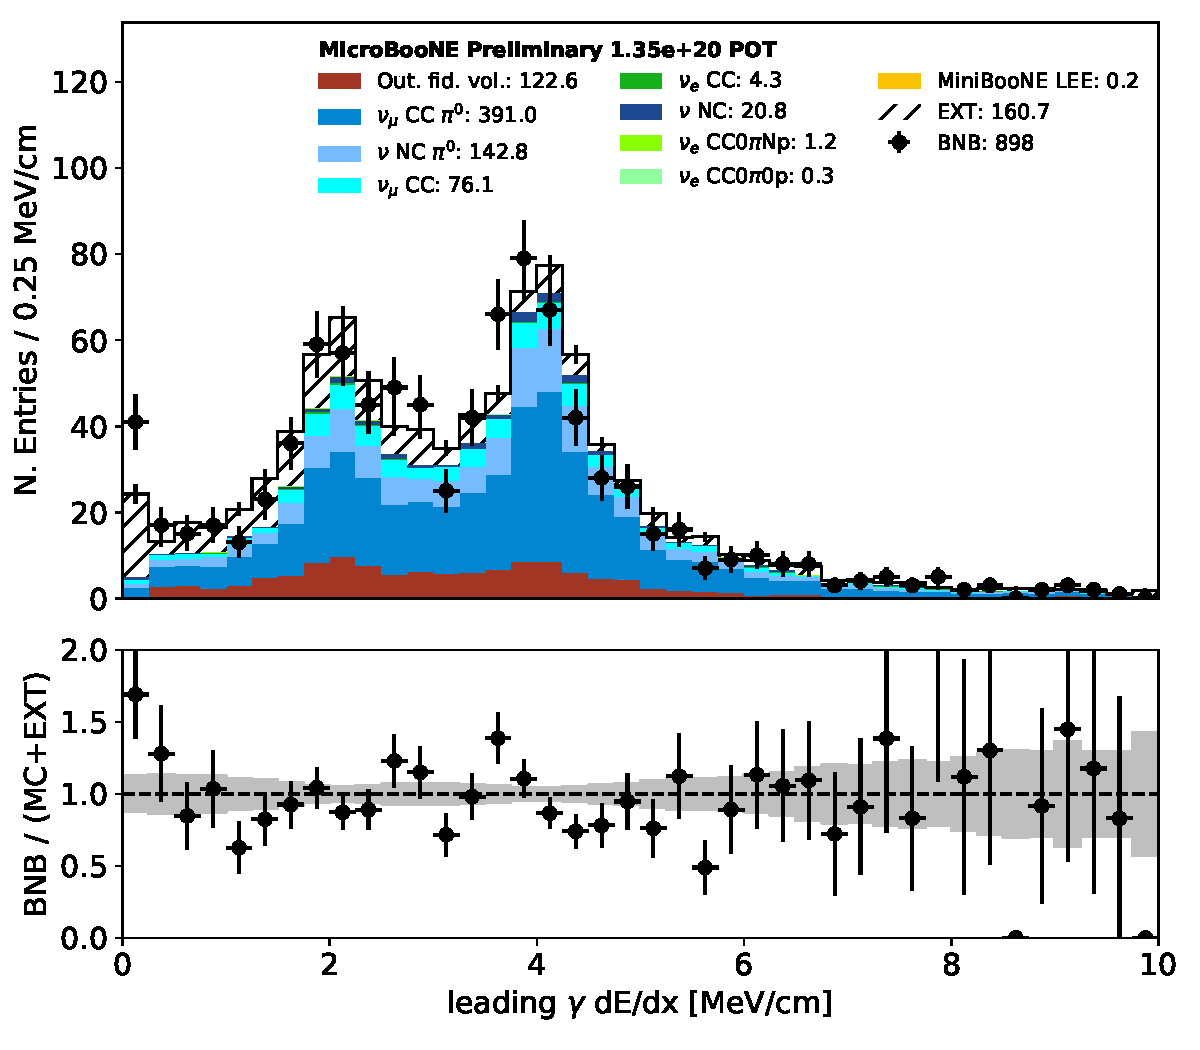
\includegraphics[width=1.00\textwidth]{pi0/pi0_dedx1_fit_Y_01152020_scaled_RUN1.pdf}
    %\caption{\label{fig:pi0:dedx:RUN1:leading} Run 1 leading shower.}
    \end{subfigure}
    \begin{subfigure}[b]{0.38\textwidth}
    \centering
    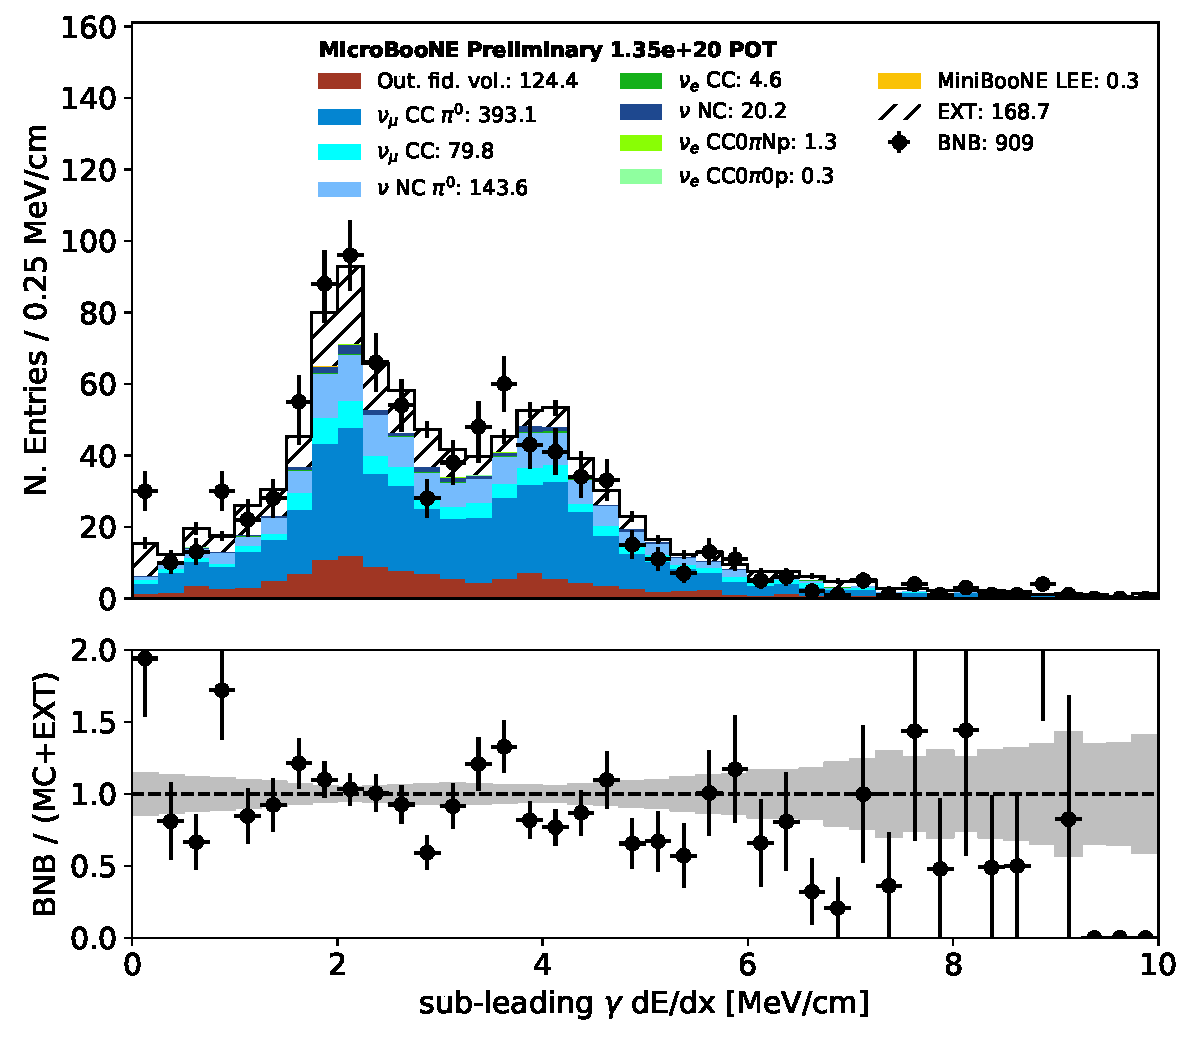
\includegraphics[width=1.00\textwidth]{pi0/pi0_dedx2_fit_Y_01152020_scaled_RUN1.pdf}
    %\caption{\label{fig:pi0:dedx:RUN1:subleading} Run 1 sub-leading shower.}
    \end{subfigure}
    
    \begin{subfigure}[b]{0.38\textwidth}
    \centering
    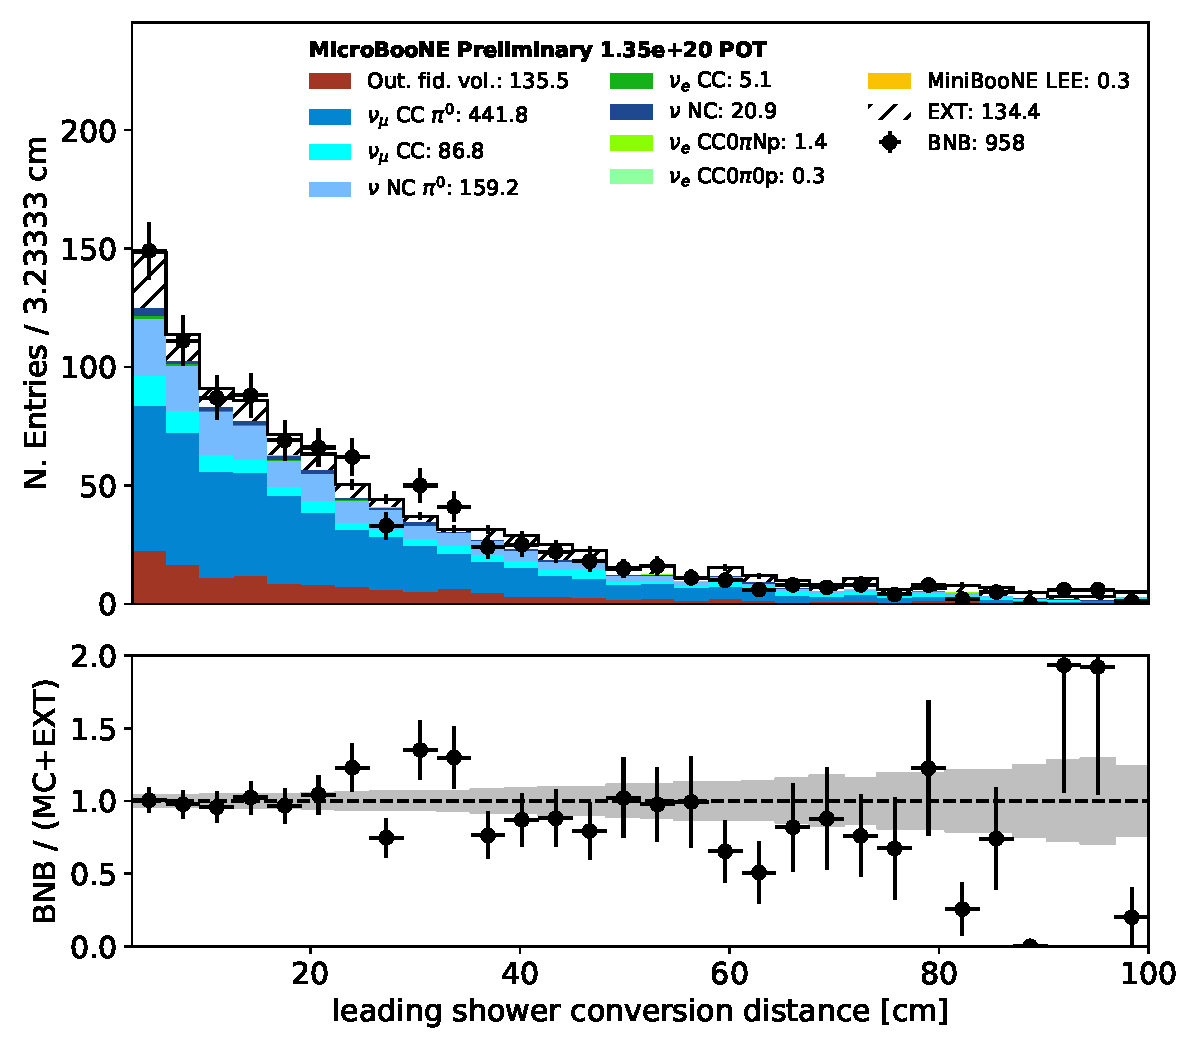
\includegraphics[width=1.00\textwidth]{pi0/pi0_radlen1_01152020_inputs_RUN1.pdf}
    %\caption{\label{fig:pi0:dedx:RUN1:leading} Run 1 leading shower.}
    \end{subfigure}
    \begin{subfigure}[b]{0.38\textwidth}
    \centering
    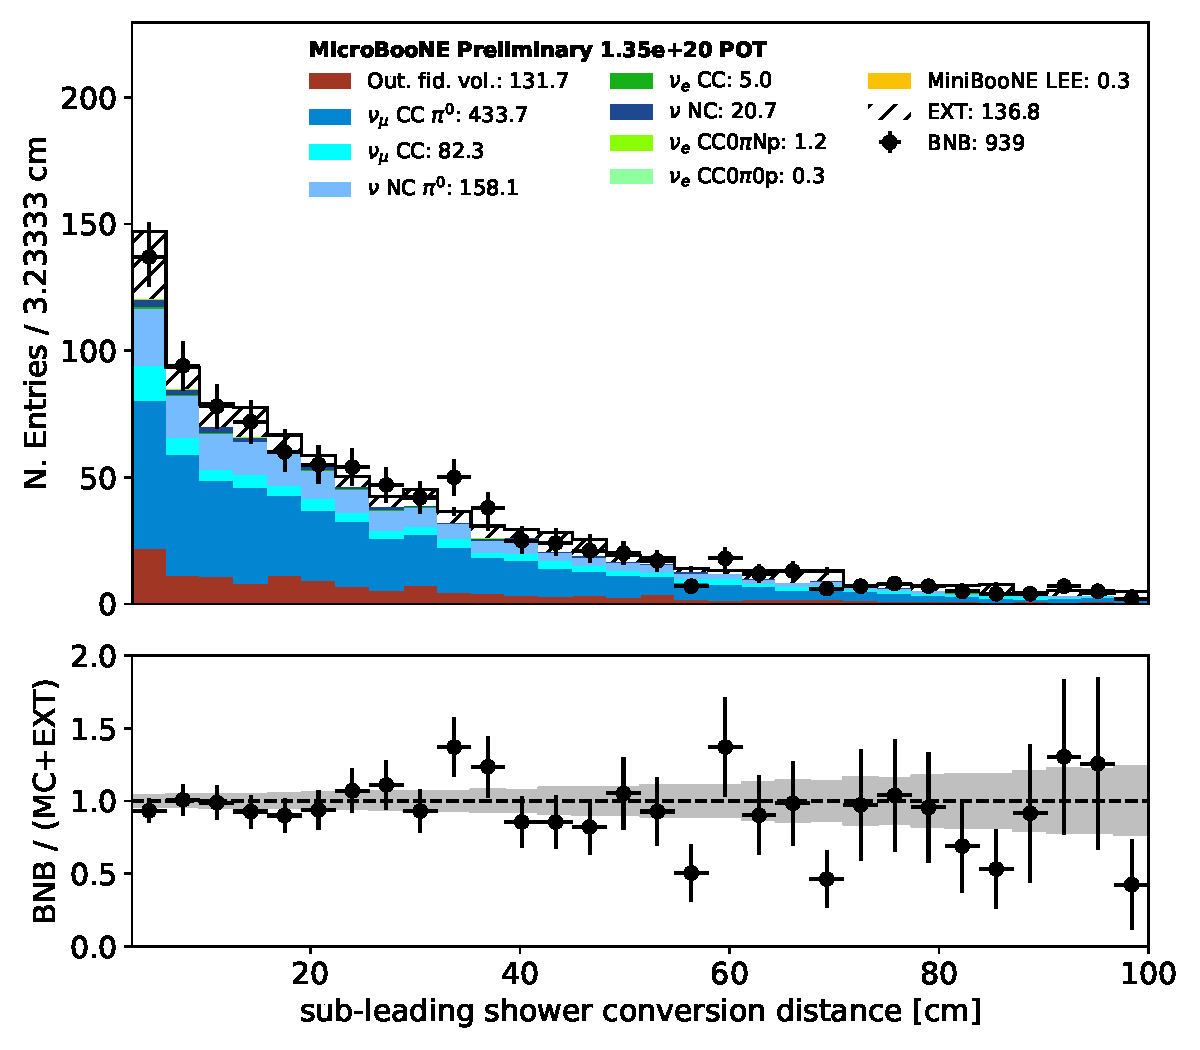
\includegraphics[width=1.00\textwidth]{pi0/pi0_radlen2_01152020_inputs_RUN1.pdf}
    %\caption{\label{fig:pi0:dedx:RUN1:subleading} Run 1 sub-leading shower.}
    \end{subfigure}
    
    \begin{subfigure}[b]{0.38\textwidth}
    \centering
    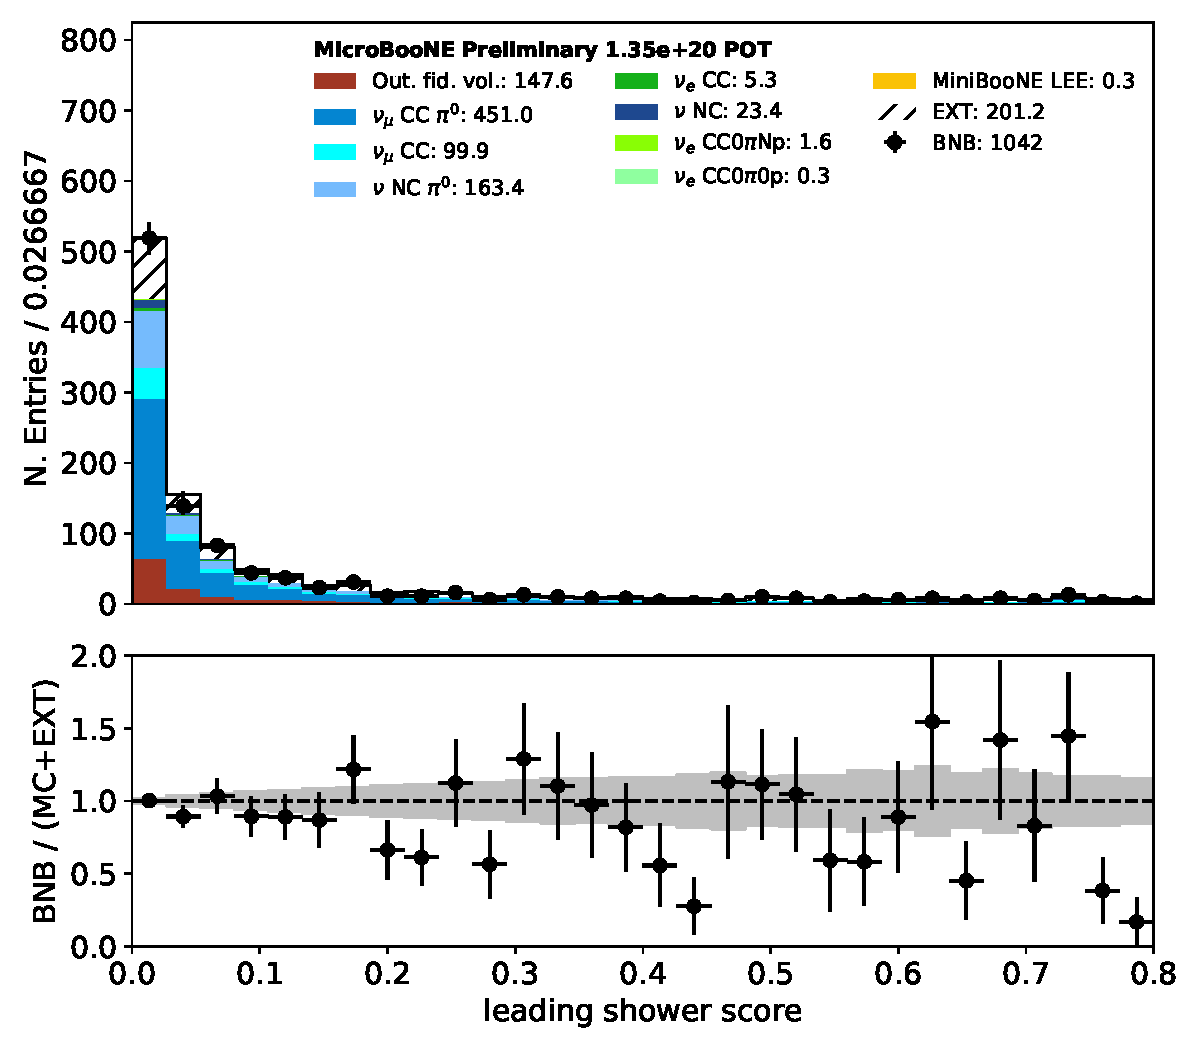
\includegraphics[width=1.00\textwidth]{pi0/pi0_shrscore1_01152020_inputs_RUN1.pdf}
    %\caption{\label{fig:pi0:dedx:RUN1:leading} Run 1 leading shower.}
    \end{subfigure}
    \begin{subfigure}[b]{0.38\textwidth}
    \centering
    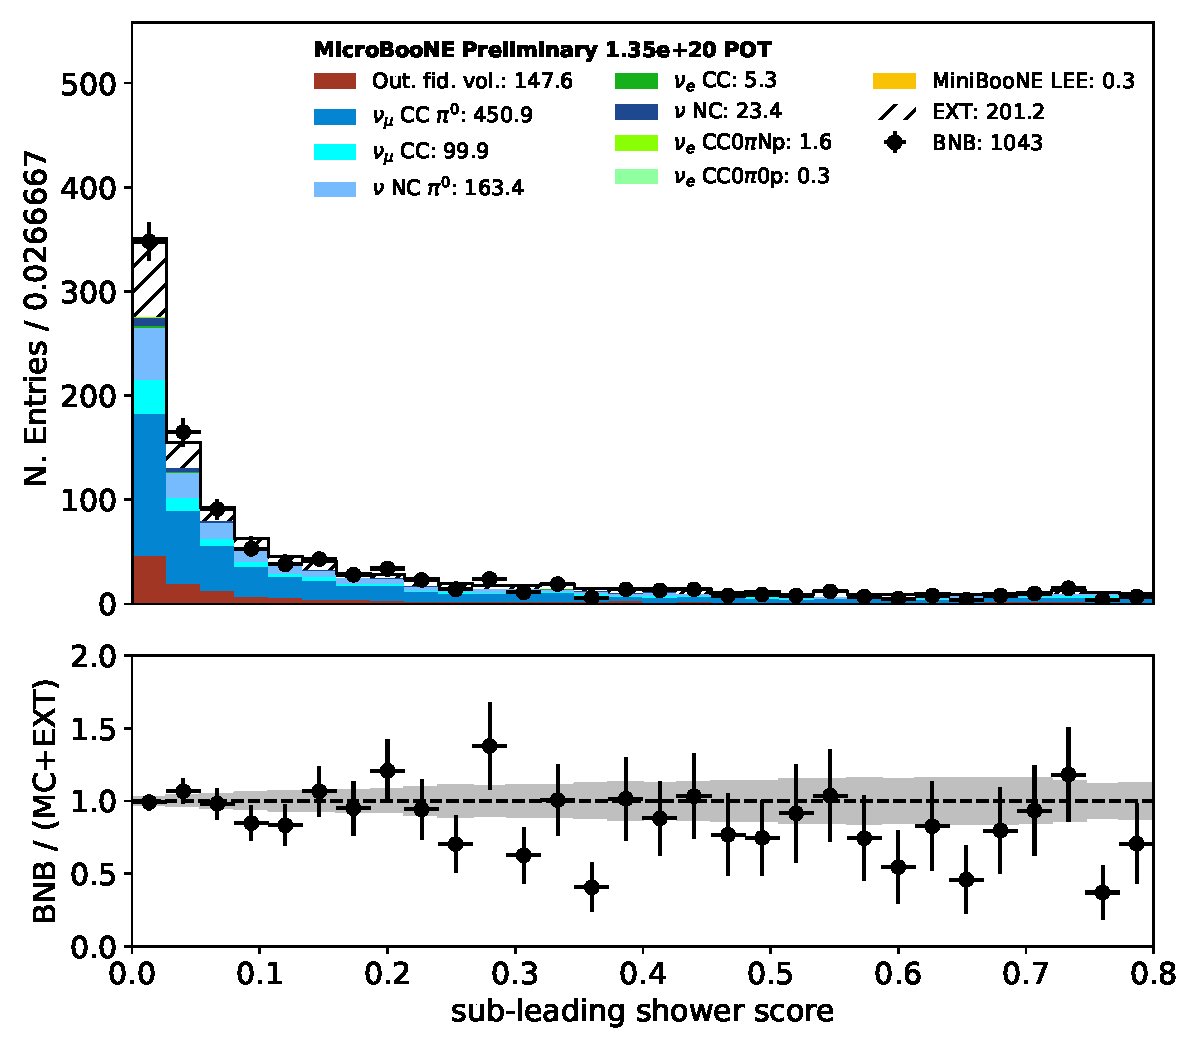
\includegraphics[width=1.00\textwidth]{pi0/pi0_shrscore2_01152020_inputs_RUN1.pdf}
    %\caption{\label{fig:pi0:dedx:RUN1:subleading} Run 1 sub-leading shower.}
    \end{subfigure}
    
    \begin{subfigure}[b]{0.38\textwidth}
    \centering
    \includegraphics[width=1.00\textwidth]{pi0/shrmoliereavg_01152020_scaled_RUN3.pdf}
    %\caption{\label{fig:pi0:dedx:RUN1:leading} Run 1 leading shower.}
    \end{subfigure}
    \begin{subfigure}[b]{0.38\textwidth}
    \centering
    \includegraphics[width=1.00\textwidth]{pi0/trkpid_01152020_scaled_RUN3.pdf}
    %\caption{\label{fig:pi0:dedx:RUN1:subleading} Run 1 sub-leading shower.}
    \end{subfigure}
    
\caption{\label{fig:pi0:datamc}Reconstructed d$E$/d$x$ for leading and sub-leading showers.}
\end{center}
\end{figure}

\subsection{Anti-BDT sample}
\par An anti-BDT filter was developed with the goal of isolating $\nu_e$ like backgrounds that could help study in detail data-mc agreement for events that are close to, but not in the $\nu_e$ signal region. The filter selects events that pass the $\nu_e$  pre-selection but fail a past iteration of the 1$e$N$p$ BDT, in order to veto and remain blind to signal events. The filter was run on $1.5E20$ POT of Run 3 data with the goal of studying in particular detail data-mc agreement for Run3, which otherwise would be limited to $0.8E19$ POT of open data. Further documentation on the \emph{anti-BDT} filter is available in reference~\cite{bib:antiBDT}. \emph{Comparisons of distributions from this filter are to be made available in a subsequent version of this note.}

\newpage


\section{$\nu_e$ Selections}
\label{sec:nueselection}
\par This section presents the three $\nu_e$ selections which comprise the analysis. We start with describing the common variables and tools leveraged by all $\nu_e$ selections in section~\ref{sec:nueselection:variables}. Next, the \npsel (sec.~\ref{sec:nueselection:1eNp}) and \zpsel (sec.~\ref{sec:nueselection:1e0p}) channel selections are presented, starting with a description of where the two selections branch off~\ref{sec:nueselection:inputs}. Finally, the $\nu_e$ inclusive selection is presented in~\ref{sec:nueselection:inclusive}.

\subsection{Variable definitions \textcolor{green}{Elena}}
\label{sec:nueselection:variables}
\par This section describes the variables used in the $\nu_e$ selections to isolate features that are specific to events with final-state electrons. We split these variables in several categories according to the pertinence of the calorimetric or topological information used: Slice Variables, Shower, Track, Shower and Track, and Shower/Track-like  Classification Variables,  2nd Shower-Based $\pi^0$ Rejection Variables.  While table ~\ref{tab:variableSummary} summarizes all variables used with a brief description, variables that warrant a longer introduction are described below.

\par \noindent  \textbf{Slice Variables}: these variables describe general features of the reconstructed neutrino interaction or event.
\par \noindent  \textbf{Track Variables}: these variables describe the features of tracks objects.
\par \noindent \textbf{Shower Variables}:  these variables describe the features of shower objects.
\par \noindent \textbf{Shower-Track Distance Variables}: these variables are used to measure the separation in space between the leading shower and the leading track, for events where at least one track and one shower are present in the slice. 
\begin{itemize}
 \item[] \textbf{3D shower-track distance} (variable: \emph{tksh\_distance}).  This variable is the 3D distance between the shower start point and the reconstructed start point of the longest track in the slice. 
 \item[] \textbf{2D track-shower distance} (variable: \emph{trkshrhitdist2}) Due to mis-reconstruction in the 3D shower and track reconstruction, sometimes the 3D distance just defined (\emph{tksh\_distance}) is significantly smeared (up to several centimeters) even if the individual track and shower are correctly clustered. These factors decreases the track-shower separation of $\nu_e$ interactions therefore reducing the $e-\gamma$ separation power achievable. To overcome this failure specific to the 3D reconstruction, a new quantity is calculated with 2D information from the collection plane defined as the smallest 2D distance between any hits associated with the shower candidate and any hits associated with the proton candidate. This variable is therefore complementary to the quantity \emph{tksh\_distance}.
\end{itemize}



\par \noindent \textbf{Shower/Track-like  Classification Variables}: The first step in track-shower classification relies on the topological score reconstructed by Pandora (variable: \emph{shr\_score}), which utilizes inputs such as the PCA component of 3D space-points to classify PFParticles. Nonetheless, this classification is not sufficient to obtain the track-shower separation needed. To improve on this, additional variables which leverage different aspects of shower topologies are devised:

\begin{itemize}

    \item[] \textbf{Shower Track-Fitted Fraction} (variable: \emph{trfit}, figure~\ref{fig:nue:variables:trkfit}) This quantity is the fraction of the 3D spacepoints in a shower object that are successfully fit with the shower track-fitter algorithm. Tracks, comprised of a single contiguous segment, will be entirely fit, leading to a fraction of 1. Showers, with several branches and split charge deposition segments, will have a fraction that is less then one.
    \item[] \textbf{Shower Sub-Clusters} (variable: \emph{subcluster}, figure~\ref{fig:nue:variables:subcluster}) This quantity leverages the fact that EM showers are often comprised of several branches isolated by gaps caused by photons propagating through the detector medium. The variable is calculated by counting the number of isolated 2D segments of charge associated to reconstructed showers. This quantity is a sum of such clusters from all three planes.
    \item[] \textbf{Moliere ``Angle''} (variable: \emph{shrmoliereavg}, figure~\ref{fig:nue:variables:dedx}) This quantity aims to characterize the profile of reconstructed EM showers. It is computed using 3D spacepoints. For each 3D spacepoint, the angle between the shower's direction and the spacepoint is calculated. The average of all such angles is used as the variable.
    \item[] \textbf{dE/dx Variables} (variables: \emph{shr\_tkfit\_2cm\_dedx\_\{U,V,Y\}} and \emph{shr\_tkfit\_gap10\_dedx\_\{U,V,Y\}} )  These variables are computed using calorimetric information from each plane separately. The two different variables are calculated as the median d$E$/d$x$ computed over some segment of a shower's trunk. The two segments used are the first two centimeters, and the range [1,5] cm, respectively. Two reasons justify the us of both these variables. Firstly, there are cases where the first few hits of a shower merge activity from short protons, causing a large d$E$/d$x$ which hampes the ability to identify the shower as an electron. These cases are particularly relevant as backgrounds for the 1$e$0$p$ channel. Secondly, in case of photon showers, d$E$/d$x$ becomes more and more MIP-like as one moves further along the shower, especially at low energy (see figure~\ref{fig:dedxgammas:dist}).
\end{itemize}{}

\begin{figure}[H] 
\begin{center}
    \begin{subfigure}[b]{0.3\textwidth}
    \centering
    \includegraphics[width=1.00\textwidth]{nueselection/variables/trkfit.png}
    \caption{\label{fig:nue:variables:trkfit} ``trkfit'' variable }
    \end{subfigure}
    \begin{subfigure}[b]{0.3\textwidth}
    \centering
    \includegraphics[width=1.00\textwidth]{nueselection/variables/nbranch.png}
    \caption{\label{fig:nue:variables:subcluster} ``subcluster'' variable }
    \end{subfigure}
    \begin{subfigure}[b]{0.3\textwidth}
    \centering
    \includegraphics[width=1.00\textwidth]{nueselection/variables/dedx.png}
    \caption{\label{fig:nue:variables:dedx} d$E$/d$x$ variables }
    \end{subfigure}
\caption{\label{fig:nue:presel:eff} Additional shower variables defined by the analysis to improve track-shower separation.}
\end{center}
\end{figure}

\par \noindent  \textbf{Second Shower Based $\pi^0$ Rejection Variables}: %Often, one of the two EM $\gamma$ showers in $\pi^0$ events is not fully reconstructed by Pandora. In many cases, these second $\gamma$ showers are correctly identified by Pandora as belonging to the neutrino slice (reconstructed in 2D), but never fully reconstructed in 3D (see fig.~\ref{fig:nue:variables:secondshowerevd}).
Pandora's reconstruction of events containing $\pi^0$ is often imperfect. In many cases, both EM $\gamma$ showers are correctly identified as belonging to the same neutrino slice (reconstructed in 2D), but one of the showers is not fully reconstructed in 3D (see fig.~\ref{fig:nue:variables:secondshowerevd}).

To improve on our $\pi^0$ rejection, we build several variables storing information associated to the largest 2D cluster in the slice on each plane. At the moment, only collection-plane variables are used. The variables, shown graphically in figure~\ref{fig:nue:variables:secondshower}, are described in table ~\ref{tab:variableunSummary}. In the example event of figure~\ref{fig:nue:variables:secondshowerevd}, these quantities are computed for the circles black cluster of charge which represents a missed photon in the $\pi^0$ reconstruction.

\begin{figure}[H] 
\begin{center}
    \begin{subfigure}[b]{0.35\textwidth}
    \centering
    \includegraphics[width=1.00\textwidth]{nueselection/variables/secondshowerevd.png}
    \caption{\label{fig:nue:variables:secondshowerevd} unclustered shower }
    \end{subfigure}
    \begin{subfigure}[b]{0.35\textwidth}
    \centering
    \includegraphics[width=1.00\textwidth]{nueselection/variables/secondshower.png}
    \caption{\label{fig:nue:variables:secondshower}second-shower variables }
    \end{subfigure}
\caption{\label{fig:nue:variables:secondshower} Visual representation of the second shower based $\pi^0$ rejection variables. Left: example event where the second shower in a $\pi^0$ event is clustered in 2D (black hits) but not fully reconstructed in 3D. Right: reconstructed variables associated to the 2nd-shower search. The gray cone in the image represents the black cluster on the left image, for which only 2D information is accessible.}
\end{center}
\end{figure}

\begin{table}[ht]
\caption{\label{tab:variableSummary} Summary of the definition for the variables used in the analysis.}
\centering
\begin{tabular}{ m{0.08\textwidth} | m{0.25\textwidth} | m{0.6\textwidth}  }
Category & Variable Name & Description  \\
\hline

\multicolumn{1}{l|}{} & \emph{nslice} &  Number of neutrino slices identified by the \emph{SliceID}. Values are  0 or 1.\\  \cline{2-3}
\multicolumn{1}{l|}{} & \emph{reco\_nu\_vtx\_sce\_\{x,y,z\}} & Reconstructed neutrino interaction vertex in (x,y,z) coordinates. The space charged correction is applied.  \\  \cline{2-3}
\multicolumn{1}{l|}{} & \emph{n\_showers\_contained} & Number of showers with a starting point within the fiducial volume. \\  \cline{2-3}
\multicolumn{1}{l|}{} & \emph{n\_tracks\_contained} & Number of tracks fully contained in the fiducial volume.  \\  \cline{2-3}
\multicolumn{1}{l|}{} & \emph{contained\_fraction} & Hits in PFParticles contained in the fiducial volume over the total number of clustered hits in the slice.  \\  \cline{2-3}
\parbox[t]{2mm}{\multirow{4}{*}{\rotatebox[origin=c]{90}{Slice}}} & \emph{hits\_ratio} & Ratio between hits from showers and total number of hits in the slice. \\  \cline{2-3}
\multicolumn{1}{l|}{} & \emph{CosmicIP} & Closest distance between shower start and space points associated to tracks flagged as cosmics. \\  \cline{2-3}
\multicolumn{1}{l|}{} & \emph{crtveto} & Boolean variable checking if the event passes the CRT veto. \\  \cline{2-3}
\multicolumn{1}{l|}{} & \emph{\_closestNuCosmicDist} &  3D distance between the reconstructed neutrino vertex and the closest CRT-tagged cosmic track. \\  \cline{2-3}
\multicolumn{1}{l|}{} & \emph{slclustfrac} & Fraction of hits in the slice that are fully reconstructed to 3D particles. \\  \cline{2-3}
\multicolumn{1}{l|}{} & \emph{nObjHits\_\{U,V,Y\}} & Number of hits associated with the object on each plane.\\  \cline{2-3}
\hline

\hline
\multicolumn{1}{l|}{} & \emph{pfp\_generation} & The generation of the PFParticle according to Pandora: the neutrino has generation 1, it's direct daughters 2, and further decay products 3 or higher.\\  \cline{2-3}
\multicolumn{1}{l|}{} & \emph{trkpid}  &  Proton-muon LLR particle identification. \\  \cline{2-3}
\parbox[t]{2mm}{\multirow{4}{*}{\rotatebox[origin=c]{90}{Track, Shower and Their Separation}}}  & \emph{shr\_energy\_tot\_cali}  & Sum  of  the  energy  of  the  calibrated  showers  (in  GeV). Used  only  at pre-selection as a ``Michel veto”.\\  \cline{2-3}
\multicolumn{1}{l|}{} & \emph{shr\_score} & Pandora  SVM track/shower score for the leading shower.\\  \cline{2-3}
\multicolumn{1}{l|}{}  & \emph{tksh\_distance}  & Distance between leading shower and longest track start points.\\  \cline{2-3}
\multicolumn{1}{l|}{} & \emph{tksh\_angle}  & Angle  between  leading  shower   and  longest  track directions.\\  \cline{2-3}
\multicolumn{1}{l|}{} & \emph{merge\_bestdist}  & Distance between shower start point and track start (or end) point for the track in the slice that best matches the direction of the shower.\\  \cline{2-3}
\multicolumn{1}{l|}{} & \emph{trfit} & Fraction of the 3D spacepoints successfully fitted with the shower track-fitter algorithm. \\  \cline{2-3}
\multicolumn{1}{l|}{} & \emph{subcluster} & Number of isolated 2D segments of charge associated to a reconstructed shower on all three planes  \\  \cline{2-3}
\multicolumn{1}{l|}{} & \emph{shrmoliereavg} &  Average angle between the shower’s direction and its 3D spacepoints.    \\ \cline{2-3}
\multicolumn{1}{l|}{} & \emph{shr\_tkfit\_gap10\_dedx\_\{U,V,Y\}}  & Median dE/dx computed over the [1,5] cm of the shower’s  trunk. \\ \cline{2-3}
\multicolumn{1}{l|}{} & \emph{shr\_tkfit\_2cm\_dedx\_\{U,V,Y\}}  & Median dE/dx computed  over  the first 2 cm of the shower’s  trunk. \\ \cline{2-3}
\multicolumn{1}{l|}{} & \emph{shower\_vtx\_dist} & Distance between the shower start and the neutrino vertex.\\ \cline{2-3}
\multicolumn{1}{l|}{} & \emph{ismerged} & Check if a proton is merged at the beginning of a shower.\\ \cline{2-3}
\hline
\hline
\multicolumn{1}{l|}{} & \emph{secondshower\_Y\_nhit} & Number of hits in the collection plane of the largest cluster associated to the  recovered 2nd shower  \\  \cline{2-3}
\parbox[t]{2mm}{\multirow{4}{*}{\rotatebox[origin=c]{90}{Second Shower}}}  & \emph{secondshower\_Y\_dot} &  Dot product between the vector connecting the vertex to the closest hit in cluster and the charge-weighted cluster direction w.r.t. closest hit in cluster \\  \cline{2-3}
\multicolumn{1}{l|}{} & \emph{anglediff\_Y} & 2D angle difference in the collection plane between the 2nd shower and the 1st shower cluster  (cluster direction defined as charge-weighted direction of cluster w.r.t. vertex) \\ \cline{2-3}
\multicolumn{1}{l|}{} & \emph{secondshower\_Y\_vtxdist} & 2D distance from vertex for the largest 2D cluster associated to the  recovered 2nd shower in the collection plane \\
\hline
\end{tabular}
\label{tab:variableSummary}
\end{table}

\clearpage

\subsection{Input to \npsel and \zpsel and channel orthogonality \textcolor{green}{David + Sophie P.R. Elena} }
\label{sec:nueselection:inputs}

The 1$e$N$p$ and 1$e$0$p$ selections rely on a common pre-selection which requires the presence of at least one reconstructed and contained EM shower (figure~\ref{fig:nue:presel:nshower}) with reconstructed energy above 70 MeV (figure~\ref{fig:nue:presel:shrenergy}). This second cut applies as a Michel-electron veto, as the majority of events which do not pass this cut are associated to cosmic or $\nu_{\mu}$ induced $\mu \rightarrow e$ Michel electrons. The two selections are subsequently split: we require the presence of at least one proton candidate for the N$p$ channel and the absence of proton candidates the 0$p$ channel. Reconstructed tracks (track-shower score $> 0.5$) are defined as proton-candidates if they are fully contained,  have a \texttt{trkpid} score $< 0$ \textcolor{blue}{I don;t think we've defined that trackpid<0 is protons, we should in a previous paragraph}, and a value of \texttt{tksh\_angle} $> -0.9$. The second condition requires that the track be proton-like according to the PID tool~\ref{subsec:loglikelihoodpid}, while the third excludes tracks reconstructed back-to-back to the electron candidate, generally due to mis-reconstruction. For events with more than one reconstructed track, these requirements are applied on the longest track.

\begin{figure}[H] 
\begin{center}
    \begin{subfigure}[b]{0.3\textwidth}
    \centering
    \includegraphics[width=1.00\textwidth]{nueselection/n_showers_contained_01132020_RUN1.pdf}
    \caption{\label{fig:nue:presel:nshower} }
    \end{subfigure}
    \begin{subfigure}[b]{0.3\textwidth}
    \centering
    \includegraphics[width=1.00\textwidth]{nueselection/n_tracks_contained_01132020_RUN1.pdf}
    \caption{\label{fig:nue:presel:ntrack} }
    \end{subfigure}
    \begin{subfigure}[b]{0.3\textwidth}
    \centering
    \includegraphics[width=1.00\textwidth]{nueselection/shr_energy_tot_cali_01132020_RUN1.pdf}
    \caption{\label{fig:nue:presel:shrenergy} }
    \end{subfigure}
\caption{\label{fig:nue:presel}Variables input to the common $\nu_e$ N$p$ and 0$p$ pre-selections.}
\end{center}
\end{figure}

\par The efficiencies of the 1$e$N$p$ and 1$e$0$p$ channels at the point where the selections diverge are shown in figure~\ref{fig:nue:presel:eff}. Efficiencies are presented as a function of true neutrino energy (fig.~\ref{fig:nue:presel:eff:nu}), proton KE (fig.~\ref{fig:nue:presel:eff:proton}), and electron energy (fig.~\ref{fig:nue:presel:eff:elec}). Each plot shows in black the efficiency for the common pre-selection (before requirements on protons are imposed) relative to all intrinsic $\nu_e$ events. The efficiencies for the  1$e$N$p$ and 1$e$0$p$ selections relative to true N$p$ and 0$p$ events are shown in blue and red respectively.
Shaded histograms in red and blue show the stacked truth-level distributions for N$p$ and 0$p$ events for the variables being plotted. It is important to observe that the reconstruction efficiency for 1$e$N$p$ events is significantly lower then that of 1$e$0$p$ events at this pre-selection stage. This is caused by the additional requirement of the presence of a proton-like track in the final state. The strong energy dependence for the efficiency in tagging protons is shown in figure~\ref{fig:nue:presel:eff:proton}. While requiring the presence of a final-state proton lowers the efficiency, this requirement has a significant impact on the selection's ultimate purity.

\begin{figure}[H] 
\begin{center}
    \begin{subfigure}[b]{0.3\textwidth}
    \centering
    \includegraphics[width=1.00\textwidth]{nueselection/nu_RUN1.pdf}
    \caption{\label{fig:nue:presel:eff:nu} }
    \end{subfigure}
    \begin{subfigure}[b]{0.3\textwidth}
    \centering
    \includegraphics[width=1.00\textwidth]{nueselection/proton_RUN1.pdf}
    \caption{\label{fig:nue:presel:eff:proton} }
    \end{subfigure}
    \begin{subfigure}[b]{0.3\textwidth}
    \centering
    \includegraphics[width=1.00\textwidth]{nueselection/elec_RUN1.pdf}
    \caption{\label{fig:nue:presel:eff:elec} }
    \end{subfigure}
\caption{\label{fig:nue:presel:eff} $\nu_e$ pre-selection efficiencies split by final-state topology as a function of different truth variables. }
\end{center}
\end{figure}

\subsection{\npsel Channel \textcolor{green}{David + Giuseppe ... PR Elena}}
\label{sec:nueselection:1eNp}

The 1$e$N$p$ channel is the most sensitive to the MiniBooNE eLEE signal as it contains a large fraction of the signal events and allows for selection requirements based both on showers and tracks. Since $\nu_e$ charge-current interactions are O(1\%) in the BNB and a large cosmic background is present, a high-purity selection is needed to achieve a sizeable signal sensitivity; the necessary trade-off is that the final signal efficiency will be low.

The section is organized as follows. We first define a set of minimal requirements (``preselection") to obtain a high statistics sample used to monitor the data-MC agreement of the selection variables;
the events at the preselection stage are dominated by cosmic and neutrino backgrounds. We then define two alternative selections, one based on a simple box-cut approach and one on boosted decision trees (BDT); the BDT approach is expected to be the most sensitive, while box-cuts provide a robust reference selection. Finally, we compare all presented selections in terms for their signal efficiency and purity.

\subsubsection{Preselection}

At preselection stage we apply the minimum set of requirements so that all selection variables can be defined, plus the containment and a minimum shower energy to reject Michel electrons (Table~\ref{tab:1eNp:presel}).

\begin{table}[h!]
\centering
\setlength{\tabcolsep}{10pt}
\renewcommand{\arraystretch}{1.25}
 \begin{tabular}{| c | c |} 
 \hline
 Cut goal & Cut definition \\
 \hline\hline
Cosmic rejection & nslice = 1 \\
 \hline
\multirow{2}{*}{Signal~topology} & n\_tracks\_contained $>$ 0 \\
 & n\_showers\_contained $>$ 0 \\
 \hline
Containment & contained\_fraction $>$ 0.9 \\
 \hline
Michel rejection & shr\_energy\_tot\_cali $>$ 0.07 GeV \\
 \hline
 \end{tabular}
 \caption{\label{tab:1eNp:presel} Preselection requirements for the \npsel selection.}
\end{table}

The relative fraction of EXT events at this stage is roughly 25\%, so we can look at all selection variables in data and MC in a neutrino-dominated sample with the open Run1 and Run3 data sets. We typically see very good agreement, which rules out major problems related to POT-scaling, detector modeling, inclusive cross-section. \emph{The main exception are dEdx variables that show some tension due to the incomplete calibration (\textcolor{blue}{see figure [add dedx figure]} and  Sec.~\ref{sec:controls:pi0} for more details) to be finalized the near future.} The full list of plots can be found in Appendix~\ref{sec:datamc:plots}. Figure~\ref{fig:1eNp:prsel} shows the level of agreement for the reconstructed neutrino energy variable. 

\begin{figure}[ht] 
\begin{center}
    \begin{subfigure}[b]{0.45\textwidth}
    \centering
    \includegraphics[width=1.00\textwidth]{1eNp/reco_e_01162020_RUN1.pdf}
    \caption{\label{fig:1eNp:prsel:RUN1} RUN 1}
    \end{subfigure}
    \begin{subfigure}[b]{0.45\textwidth}
    \centering
    \includegraphics[width=1.00\textwidth]{1eNp/reco_e_01162020_RUN3.pdf}
    \caption{\label{fig:1eNp:prsel:RUN1} RUN 3}
    \end{subfigure}
\caption{\label{fig:1eNp:prsel}Reconstructed neutrino energy after pre-selection for the \npsel channel.}
\end{center}
\end{figure}

\subsubsection{Box-cuts}

On top of preselection requirements, we define a robust selection based on box cuts targeting high $\nu_e$ purity, especially at lower energy.
We present here cuts in different categories according to the background they primarily suppress; however,  the following description should be regarded as a simplification since some variables are effective against multiple backgrounds.


The requirement of a proton-like track is a very effective tool for cosmic rejection: this requirement rejects more than 90\% of the cosmics that pass pre-selection. We aim at rejecting more cosmic-induced events by requiring a large distance of the neutrino vertex from clear cosmic tracks. 

The next goal is to suppress events from $\nu_\mu$ charged current interactions; for this purpose, we impose tight quality requirements on the shower object and we require the shower hits to be the dominant contribution in the slice. These requirements rely on several variables aiming at separating EM showers from single-particle tracks, i.e. shr\_score, shrmoliereavg, trkfit, subcluster. 

At this stage, most of the selected events contain neutrino-induced electromagnetic activity. Thus, the main background left to tackle is  $\pi^0$ events. For $\pi^0$ rejection, we employ a series of requirements based on the different topology and energy deposition of electrons and photons. We first require the presence of only one shower-like PFParticle starting at a short distance from the track start in the event. Then, we require that the energy loss at the start of the electron shower is be compatible with a single MIP. Many dEdx variable definitions are possible, and information from all TPC planes can be used. However, due to detector and reconstruction limitations, there is not a single definition that provides a sharp separation between electrons and photons. In order to obtain a good background rejection without large efficiency losses, we choose to apply a loose MIP cut on two different dEdx definitions (described in Sec.~\ref{sec:nueselection:variables}). The loose MIP requirement enforces that there is at least one hit in the collection plane in the probed range, and that the dEdx is not consistent with two or more MIPs in any plane. Finally, the single shower requirement is reinforced with a 2nd shower veto based on clusters in the collection plane that are not matched to any PFParticle.

The last cut aims at rejecting misreconstructed events and requires that the track and shower are not aligned. For reference, the full list of cuts is in Table~\ref{tab:1eNp:boxcut}.

The resulting reconstructed \nue energy after the BDT selection is shown in Figure~\ref{fig:1eNp:box:RUN1}. Two events are found in the available $4.07E19$ POT dataset from Run1, with an expectation of 2.3 from the simulation. Both events appear to be good $\nu_e$ candidates (consistent with the level of purity expected), and are reconstructed with $\sim 1.1$ GeV of energy

\begin{table}[h!]
\centering
\setlength{\tabcolsep}{10pt}
\renewcommand{\arraystretch}{1.25}
 \begin{tabular}{| c | c |} 
 \hline
 Cut goal & Cut definition \\
 \hline\hline
\multirow{2}{*}{Cosmic~rejection} & CosmicIP $>$ 20. \si{\cm} \\
& trkpid $<$ -0.02 \\
 \hline
\multirow{4}{*}{$\nu_\mu$~rejection} & hits\_ratio $>$ 0.60 \\
 & shr\_score $<$ 0.275 \\
& shrmoliereavg $>$ 2\si{\degree} and shrmoliereavg $<$ 9\si{\degree} \\
& trkfit $<$ 0.45 or subcluster $>$ 6 \\
 \hline
\multirow{6}{*}{$\pi^0$~rejection} & n\_showers\_contained = 1 \\
& tksh\_distance $<$ 3.5 \si{\cm} \\
& shr\_tkfit\_2cm\_dedx\_Y $>$ 0 and shr\_tkfit\_2cm\_dedx\_\{U,V,Y\} $<$ 4.0 \si{\MeV}/\si{\cm} \\
& shr\_tkfit\_gap10\_dedx\_Y $>$ 0 and shr\_tkfit\_gap10\_dedx\_\{U,V,Y\} $<$ 4.5 \si{\MeV}/\si{\cm} \\
& (secondshower\_Y\_nhit $\leq$ 8 or secondshower\_Y\_dot $\leq$ 0.8 or \\
&  anglediff\_Y $\leq$ 40 or secondshower\_Y\_vtxdist $\geq$ 100 \si{\cm}) \\
 \hline
Misreconstruction & tksh\_angle $>$ -0.9 and tksh\_angle $<$ 0.7 \\
 \hline
 \end{tabular}
 \caption{\label{tab:1eNp:boxcut} Box cut requirements for the \npsel selection.}
\end{table}

\begin{figure}[ht]
\begin{center}
\includegraphics[width=0.45\textwidth]{1eNp/reco_e_01162020_box_RUN1.pdf}
\caption{\label{fig:1eNp:box:RUN1} Reconstructed energy spectrum for events passing the box-cuts for \npsel channel.}
\end{center}
\end{figure}

\begin{figure}[H] 
\begin{center}
    \begin{subfigure}[b]{0.45\textwidth}
    \centering
    \includegraphics[width=1.00\textwidth]{1eNp/1eNp_box_evd1.png}
    \caption{\label{fig:1eNp:box:evd1}1.19 GeV [reco] $\nu_e$ candidate}
    \end{subfigure}
    \begin{subfigure}[b]{0.45\textwidth}
    \centering
    \includegraphics[width=1.00\textwidth]{1eNp/1eNp_box_evd2.png}
    \caption{\label{fig:1eNp:box:evd2}1.15 GeV [reco] $\nu_e$ candidate}
    \end{subfigure}
\caption{\label{ffig:1eNp:box:evd} \npsel candidates from the open $4eE19$ Run1 open dataset. Two data events are found when }
\end{center}
\end{figure}

\subsubsection{BDT}

Alternatively to the box cut approach, a selection based on Boosted Decision Tree (BDT) algorithms has been developed. This selection is expected to be the most sensitive to low-energy \nue events since BDTs are able to learn additional information from the data and return a response variable that is highly discriminating between signal and background. 

\emph{While the development of the BDT selection is fairly advanced, a few steps are needed before it is finalized. Current limitations are mainly related to the limited size of the samples that are available for training and to the ongoing calibration of the dEdx variables used in the BDT. The limited sample size can lead to overtraining and suboptimal performance, while the missing calibration can induce small data-MC disagreements.} 

Because of these limitations, we deemed safer to consider only events that pass a loose set of cuts (Table~\ref{tab:1eNp:loosecut}) intended to reject events where one or more variables is clearly inconsistent with \nuecc interactions. The loose cuts are applied on top the of the preselection both before the BDT training and before the application of the BDT in the analysis. This selection enhances the relative population of \nuecc in the BNB overlay sample from about 1\% to more than 25\% (Fig.~\ref{fig:1eNp:loosesel}). \emph{In the final implementation of the BDT selection, the loose selection cuts may be revisited or removed}.
\begin{table}[h!]
\centering
\setlength{\tabcolsep}{10pt}
\renewcommand{\arraystretch}{1.25}
 \begin{tabular}{| c | c |} 
 \hline
 Cut goal & Cut definition \\
 \hline\hline
\multirow{2}{*}{Cosmic~rejection} & CosmicIP $>$ 20. \si{\cm} \\
& trkpid $<$ 0.1 \\
 \hline
\multirow{2}{*}{$\nu_\mu$~rejection} & hits\_ratio $>$ 0.50 \\
 & shr\_score $<$ 0.30 \\
 \hline
\multirow{2}{*}{$\pi^0$~rejection} & n\_showers\_contained = 1 \\
& tksh\_distance $<$ 6.0 \si{\cm} \\
& shr\_tkfit\_2cm\_dedx\_Y $<$ 4.0 \si{\MeV}/\si{\cm} \\
 \hline
Misreconstruction & tksh\_angle $>$ -0.9 \\
 \hline
 \end{tabular}
 \caption{\label{tab:1eNp:loosecut} Loose cut requirements for the \npsel BDT selection.}
\end{table}

\begin{figure}[H]
\begin{center}
\includegraphics[width=0.45\textwidth]{1eNp/loose_sel_perf.png}
\caption{\label{fig:1eNp:loosesel} Fraction of events in the BNB sample divided in different categories before and after the loose selection.}
\end{center}
\end{figure}

Two BDTs are trained separately to reject backgrounds with and without $\pi^0$ in the final state. The same set of training variables is used in the two BDTs, corresponding to the list of variables used in the box-cut selection. The BDT training is able to figure out which variables are most important for each background. Figure~\ref{ffig:1eNp:bdt:var} shows that shower quality variables (e.g. shr\_score, trkfit, subcluster) have higher ranking for the non-$\pi^0$ BDT, while variables such as tksh\_distance and the shower dEdx have higher importance for the $\pi^0$-BDT. It is interesting to note that the most discriminating variable in both cases is shrmoliereavg, since it can be useful to discriminate both muons in $\nu_\mu$ events (low values) and merged showers in $\pi^0$ events (large values).

\begin{figure}[H] 
\begin{center}
    \begin{subfigure}[b]{0.45\textwidth}
    \centering
    \includegraphics[width=1.00\textwidth]{1eNp/bdt_var_gain.pdf}
    \caption{\label{fig:1eNp:bdt:var:gain}}
    \end{subfigure}
    \begin{subfigure}[b]{0.45\textwidth}
    \centering
    \includegraphics[width=1.00\textwidth]{1eNp/bdt_var_rank.pdf}
    \caption{\label{fig:1eNp:bdt:var:rank}}
    \end{subfigure}
\caption{\label{ffig:1eNp:bdt:var} BDT variables importance in terms of ``total gain" \textcolor{blue}{what's the total gain?}. dEdx variables are combined for different planes (note the ``ALL" suffix). Left: total gain value. Right: ranking based on the total gain value (highest ranking=15, lowest=1).}
\end{center}
\end{figure}

The resulting response in Run1 open data are shown in Figures~\ref{fig:1eNp:bdt:nonpi0} and \ref{fig:1eNp:bdt:pi0} for the non-$\pi^0$ and $\pi^0$ BDT, respectively. The left panel shows the full response, while the right one zooms in in the high BDT score region and shows the signal enhancement in the bin with response $>$ 0.99. We cut separately on the output of the two BDTs, requiring the $\pi^0$ and non-$\pi^0$ responses to be greater than 0.995 and 0.9984, respectively. The resulting reconstructed \nue energy after the BDT selection is shown in Figure~\ref{fig:1eNp:bdt:RUN1}.

\begin{figure}[H] 
\begin{center}
    \begin{subfigure}[b]{0.45\textwidth}
    \centering
    \includegraphics[width=1.00\textwidth]{1eNp/nonpi0_score_01162020_RUN1.pdf}
    \caption{\label{fig:1eNp:bdt:nonpi0:all}}
    \end{subfigure}
    \begin{subfigure}[b]{0.45\textwidth}
    \centering
    \includegraphics[width=1.00\textwidth]{1eNp/nonpi0_score_zoom_01162020_RUN1.pdf}
    \caption{\label{fig:1eNp:bdt:nonpi0:zoom}}
    \end{subfigure}
\caption{\label{fig:1eNp:bdt:nonpi0}BDT response for non-$\pi^0$ BDT after \npsel pre-selection}
\end{center}
\end{figure}

\begin{figure}[H] 
\begin{center}
    \begin{subfigure}[b]{0.45\textwidth}
    \centering
    \includegraphics[width=1.00\textwidth]{1eNp/pi0_score_01162020_RUN1.pdf}
    \caption{\label{fig:1eNp:bdt:pi0:all}}
    \end{subfigure}
    \begin{subfigure}[b]{0.45\textwidth}
    \centering
    \includegraphics[width=1.00\textwidth]{1eNp/pi0_score_zoom_01162020_RUN1.pdf}
    \caption{\label{fig:1eNp:bdt:pi0:zoom}}
    \end{subfigure}
\caption{\label{fig:1eNp:bdt:pi0}BDT response for $\pi^0$ BDT after \npsel pre-selection}
\end{center}
\end{figure}

\begin{figure}[H]
\begin{center}
\includegraphics[width=0.45\textwidth]{1eNp/reco_e_01162020_bdt_RUN1.pdf}
\caption{\label{fig:1eNp:bdt:RUN1}BDT-based selection for \npsel with cuts at 0.995 and 0.9984 for the $\pi^0$ and non-$\pi^0$ variables respectively.}
\end{center}
\end{figure}

\subsubsection{Performance of \npsel selections}

Figure~\ref{fig:1eNp:effpur:RUN1} shows the efficiency of the \npsel selections as a function of the neutrino energy and reports the corresponding intrinsic \npsel purity in the reconstructed energy range [0.2, 1.0] \si{\GeV}. The efficiency is already low at preselection level, especially for neutrino energies below 0.8 \si{\GeV}. This demonstrates how challenging it is to properly identify and reconstruct such events. The loose cuts then are able to improve the purity by one order of magnitude at the price of a 50\% reduction in efficiency. The BDT (box cut) selection then further improve the purity by a factor 7.4 (6.6) with a $\sim$30\% (50\%) reduction in efficiency. With the full 10.1e20 POT dataset, the expected number of MiniBooNE LEE signal events identified with the box cut selection is about 8, and increase to almost 11 with the BDT selection.

\emph{Figures~\ref{fig:1eNp:box:RUN1} and \ref{fig:1eNp:bdt:RUN1} show that the background to the \npsel events is in large fraction constituted by single events with large weight. This due to the relatively small size of the inclusive BNB sample. Note instead that the $\pi^0$ backgrounds are smoother since they come from larger dedicated samples. We are currently processing the additional background samples just produced by the collaboration. We thus plan to revisit the box cut and BDT selections after such samples will become available and after a residual calibration is applied to the dEdx variables.}


\begin{figure}[H]
\begin{center}
\includegraphics[width=0.45\textwidth]{1eNp/effpur_1eNp_cut_bdt.pdf}
\caption{\label{fig:1eNp:effpur:RUN1} Efficiency of different selections for true contained \npsel events. The legend quotes the purity of intrinsic \npsel in the reconstructed energy range [0.2, 1.0] \si{\GeV} (where a possible MiniBooNE LEE signal is not considered).}
\end{center}
\end{figure}

\subsection{1$e$0$p$ Channel \textcolor{green}{Sophie, Ivan}}
\label{sec:nueselection:1e0p}
The 1e0p channel is an important topology that can be used to constrain uncertainties associated with the 1eNp selection.  In particular, it can be used to constrain uncertainties associated with low energy protons, such as the modeling of the proton multiplicity and kinematics produced by neutrino interactions, and their reconstruction efficiencies.  This selection is very sensitive to the neutrino interaction modeling, which makes it a useful way to constrain these systematics with data.  In MCC8, there were twice as many events in this channel as in MCC9, and half of the  neutrinos below 0.8 GeV were in this channel.

This sample also contains additional low energy electron neutrinos which can be used as signal in the eLEE search.  This signal is also complementary because it is part of the signal that MiniBooNE measured; their signal was 1eXp0pi, or the sum of the 1eNp0pi and 1e0p0pi samples, so including this sample makes it possible to fully reproduce the event topologies observed by MinibooNE.    

\subsubsection{Tools Unique to 0p Selection}

The 1e0p sample is able to constrain systematic uncertainties in the Np sample because it is fully orthogonal with the Np selection.  This will allow migrations in a simulataneous fit, as described in section XX.  This also makes it possible to recover neutrino events that fail the Np selection cuts.  One of the tools used to do this is shower-track merging.  In some events the shower trunk is mis-reconstructed as a track.  These events are typically discarded immediately in the Np selection, either by a cut on the angle between the track and the shower, or the track PID.  The track-shower merging is a tool designed to recover these events.

In the track-shower merging, the tracks in a neutrino slice are matched with the most energetic shower.  The angle between the track and shower and the distance between both the start and end point of the track and the start point of the shower are evaluated.  The track that best aligns in direction with the shower is selected to merge with the shower.  Then the distance from the start point of the shower to both the start and end point of this track is evaluated.  The smaller distance is stored as merge\_bestdist, which is a measure of the closest distance between the track and the shower. If an event has one contained track and one contained shower, but fails the Np selection cuts at either the shower-track angle or track PID stage, and the merged track is within 2cm of the start point of the shower then the event is recovered in the 1e0p selection.  As of December 20th, this corresponded to a 20\% increase in selected 1e0p events.

This tool could be expanded in the future to re-calculate for de/dx along the new track/shower length, or to re-fit the entire event as a shower.

\subsubsection{Pre-selection}
A basic set of pre-selection cuts are defined for the 1e0p selection.  These require that the selection variables are defined, and all potential 1eNp events, including those included with track-shower merging are included.  The pre-selection also includes a cut on the shower energy to remove decay electrons from cosmic muons.

The 1e0p pre-selection is:
\begin{itemize}
    \item nslice = 1
    \item slpdg = 12
    \item n\_showers\_contained = 1
    \item n\_tracks\_contained == 0 or (n\_tracks\_contained==1 and (tksh\_angle<-0.9 or trkpid > 0.1) and merge\_bestdist<2)
    \item shr\_energy\_tot\_cali $>$ 0.07
\end{itemize}

Using this pre-selection, both box cuts and a BDT selection have been developed for the 1e0p channel.

\subsubsection{Box cut selection}

A box cut selection has been developed to select 1e0p events.  The selection cuts are designed to target the main backgrounds.  The strict fiducial volume from the CC inclusive analysis (cite cc inclusive paper) has been implemented to reduce the backgrounds associated with dirt and single showers from backgrounds entering the FV.   In addition to the CRT cuts there is also a cut on CosmicIP which directly targets removing cosmics.  In order to remove muon neutrino, and non-showering backgrounds there are also cuts on the shower profile and the number of subclusters in the shower.  A second shower search for hits in the Y plane is used to remove events where the second shower of a pi0 may have initially been missed.  dEdx is also used to remove pi0 backgrounds.  Two calculations are used, one which looks at the first 2 cm of the shower, and one which starts the calculation after 1 cm so that any hits from a low energy proton that may have been merged with the shower are not included in the calculation.

The 1e0p box cuts are:

\begin{itemize}
    \item nslice = 1
    \item slpdg = 12
    \item n\_showers\_contained == 1
    \item n\_tracks\_contained == 0 or (n\_tracks\_contained==1 and (tksh\_angle$<$-0.9 or trkpid $>$ 0.1) and merge\_bestdist$<$2)
    \item shr\_energy\_tot\_cali $>$ 0.1
    \item (crtveto!=1) and (\_closestNuCosmicDist $>$ 20.)
    \item (reco\_nu\_vtx\_sce\_x$>$22 and reco\_nu\_vtx\_sce\_x $<$234.35)
    \item (reco\_nu\_vtx\_sce\_y $>$ -75.1 and reco\_nu\_vtx\_sce\_y$<$75.1)
    \item ((reco\_nu\_vtx\_sce\_z$>$35 and reco\_nu\_vtx\_sce\_z$<$665) or (reco\_nu\_vtx\_sce\_z$>$785 and reco\_nu\_vtx\_sce\_z$<$941.8))
    \item shrmoliereavg $>$ 2 and shrmoliereavg $<$ 9
    \item shr\_score $<$ 0.1
    \item CosmicIP $>$ 20.
    \item (trkfit $<$ 0.45 or subcluster $>$ 6)
    \item secondshower\_Y\_nhit$<$25
    \item (shr\_tkfit\_2cm\_dedx\_Y $<$ 4 and shr\_tkfit\_2cm\_dedx\_Y $>$ 0.5)
    \item (shr\_tkfit\_gap10\_dedx\_Y$>$1 and shr\_tkfit\_gap10\_dedx\_Y$<$ 3.5)
\end{itemize}

\begin{figure}[H]
\begin{center}
\includegraphics[width=0.45\textwidth]{1e0p/reco_e_01162020_RUN3.pdf}
\caption{\label{fig:1e0p:cutbased:RUN3} Box cuts for 1e0p selection, scaled up to full data set 10.1e20 POT.}
\end{center}
\end{figure}

The reconstructed energy distribution after this selection is shown in Fig.~\ref{fig:1e0p:cutbased:RUN3}.  Note that this plot uses the new Genie model, but the cuts have not yet been optimized for the new MC.  This selection predicts 9.8 true 1e0p events in the full data set and is 27\% pure in Run 3 for electron neutrinos and the LEE.  This selection will be tuned and the work expanded to include Run 1.

\subsubsection{BDT}

A selection has also been developed by training a BDT for the 1e0p events, using a similar method to the one employed by the 1eNp analysis.  At this stage the BDT has only been trained for Run 3 events, and includes a cut on the CRT before training to remove cosmics.  This work will be expanded to include Run 1.

The BDT is trained on a loose selection of 1e0p events, which includes the pre-cuts as well as several additional requirements that comprise a "loose selection" to focus on identifying electron neutrinos.

The loose selection for the 1e0p selection is:
\begin{itemize}
    \item nslice = 1
    \item slpdg = 12
    \item n\_showers\_contained = 1
    \item n\_tracks\_contained == 0 or (n\_tracks\_contained==1 and (tksh\_angle<-0.9 or trkpid > 0.1) and merge\_bestdist<2)
    \item shr\_energy\_tot\_cali $>$ 0.07
    \item Shr\_tkfit\_2cm\_dedx\_Y$<$4
    \item Shr\_score$<$0.3
    \item cosmicIP$>$20
    \item (crtveto!=1) and (\_closestNuCosmicDist $>$ 20.)
    \item (reco\_nu\_vtx\_sce\_x$>$22 and reco\_nu\_vtx\_sce\_x $<$234.35)
    \item (reco\_nu\_vtx\_sce\_y $>$ -75.1 and reco\_nu\_vtx\_sce\_y$<$75.1)
    \item ((reco\_nu\_vtx\_sce\_z$>$35 and reco\_nu\_vtx\_sce\_z$<$665) or (reco\_nu\_vtx\_sce\_z$>$785 and reco\_nu\_vtx\_sce\_z$<$941.8))
\end{itemize}

Note that even this initial selection is somewhat strict, and comes with a drop in overall electron neutrino efficiency.  This is an initial study of the BDT performance, and it may be possible to loosen these cuts and regain efficiency without compromising the BDT selection performance. 

At this stage a single BDT has been trained for this selection, which tries to separate all backgrounds from electron neutrino signals.  Performance may be improved by using multiple BDTs which are trained for specific background topologies as is done in the 1eNp selection. 

As input the BDT uses for the most part the same variables as the box cuts.  In all cases in the BDT, however, the full three plane information is used, while it was not always found to improve the performance when using box cuts.  More information from the second shower search is also included in the BDT, such as the distance from the vertex to the second shower, and the angle between the second shower and the initial shower. The full list of variables used to train the 0p BDT is: shrmoliererms, shrmoliereavg, shr\_score, CosmicIP, subcluster, secondshower\_(U,V,Y)\_nhit, secondshower\_(U,V,Y)\_vtxdist, secondshower\_(U,V,Y)\_dot, anglediff\_(U,V,Y), shr\_tkfit\_2cm\_dedx\_(U,V,Y), shr\_tkfit\_gap10\_dedx\_(U,V,Y), trkfit, and hits\_ratio.

\begin{figure}[H]
\begin{center}
\includegraphics[width=0.45\textwidth]{1e0p/bdt_vars_Run3.png}
\caption{\label{fig:1e0p:bdtvars:RUN3} Relative importance of each variable to BDT.}
\end{center}
\end{figure}

Plot ~\ref{fig:1e0p:bdtvars:RUN3} shows the relative importance of each of these variables in the BDT.  The variables for which information from all three planes is used in the BDT are combined into one variable labeled "ALL" in this plot.  

\begin{figure}[H] 
\begin{center}
    \begin{subfigure}[b]{0.45\textwidth}
    \centering
    \includegraphics[width=1.00\textwidth]{1e0p/bkg_score_01162020_RUN3_nslice.pdf}
    \caption{\label{fig:1e0p:bdt:bkgscore:slice} After requiring a neutrino slice.}
    \end{subfigure}
    \begin{subfigure}[b]{0.45\textwidth}
    \centering
    \includegraphics[width=1.00\textwidth]{1e0p/bkg_score_01162020_RUN3_presel.pdf}
    \caption{\label{fig:1e0p:bdt:bkgscore:presel} After pre-selection.}
    \end{subfigure}
\caption{\label{fig:1e0p:bdt:bkgscore} BDT response for background BDT.}
\end{center}
\end{figure}

The BDT response after a slice, and after the 1e0p pre-selection is shown in Fig.~\ref{fig:1e0p:bdt:bkgscore}.  These show good data-MC agreement on run 3 data.

\begin{figure}[H] 
\begin{center}
    \begin{subfigure}[b]{0.45\textwidth}
    \centering
    \includegraphics[width=1.00\textwidth]{1e0p/bkg_score_01162020_RUN3_loosesel.pdf}
    \caption{\label{fig:1e0p:bdt:bkgscore:loose} Full response.}
    \end{subfigure}
    \begin{subfigure}[b]{0.45\textwidth}
    \centering
    \includegraphics[width=1.00\textwidth]{1e0p/bkg_score_01162020_RUN3_loosesel_zoom.pdf}
    \caption{\label{fig:1e0p:bdt:bkgscore:loosezoom} Zoomed in.}
    \end{subfigure}
\caption{\label{fig:1e0p:bdt:loose} BDT response for background BDT after loose selection.}
\end{center}
\end{figure}

The BDT response after the loose selection that is used for training, and to cut on for the selection is shown in Fig.~\ref{fig:1e0p:bdt:bkgscore:loose}.  Based on this plot events above 0.96 in BDT response are selected as signal.

The full set of BDT selection cuts is:
\begin{itemize}
    \item nslice = 1
    \item slpdg = 12
    \item n\_showers\_contained = 1
    \item n\_tracks\_contained == 0 or (n\_tracks\_contained==1 and (tksh\_angle<-0.9 or trkpid > 0.1) and merge\_bestdist<2)
    \item shr\_energy\_tot\_cali $>$ 0.07
    \item Shr\_tkfit\_2cm\_dedx\_Y$<$4
    \item Shr\_score$<$0.3
    \item cosmicIP$>$20
    \item (crtveto!=1) and (\_closestNuCosmicDist $>$ 20.)
    \item (reco\_nu\_vtx\_sce\_x$>$22 and reco\_nu\_vtx\_sce\_x $<$234.35)
    \item (reco\_nu\_vtx\_sce\_y $>$ -75.1 and reco\_nu\_vtx\_sce\_y$<$75.1)
    \item ((reco\_nu\_vtx\_sce\_z$>$35 and reco\_nu\_vtx\_sce\_z$<$665) or (reco\_nu\_vtx\_sce\_z$>$785 and reco\_nu\_vtx\_sce\_z$<$941.8))
    \item bkg\_score $>$ 0.96
\end{itemize}

\begin{figure}[H]
\begin{center}
\includegraphics[width=0.45\textwidth]{1e0p/reco_e_01162020_RUN3_bgbdt.pdf}
\caption{\label{fig:1e0p:bdt:RUN3} BDT selection for 1e0p events, scaled up to full data set 10.1e20 POT.}
\end{center}
\end{figure}

The reconstructed energy distribution for selected 1e0p events that pass the BDT selection are shown in Fig.~\ref{fig:1e0p:bdt:RUN3}.  Note that one event in the run 3 open data passes this selection, but it is omitted from the plot because it is scaled up to the full data set.  This selection predicts 10 true 1e0p events in the full data set, and is 49\% pure in Run 3 for electron neutrinos and the LEE.

\begin{figure}[H]
\begin{center}
\includegraphics[width=0.45\textwidth]{1e0p/efficiency_RUN3.pdf}
\caption{\label{fig:1e0p:eff:RUN3} Efficiency of 1e0p selections.  The purity quoted in the legend is calculated from 0-2 GeV in reconstructed neutrino energy.}
\end{center}
\end{figure}

The selection efficiency for the 1e0p cut-based and BDT selections are shown in Fig.~\ref{fig:1e0p:eff:RUN3}.  The BDT selection is both more efficient and more pure. 

\clearpage

\subsection{$\nu_e$ CC Inclusive selection \textcolor{green}{Wouter}}
\label{sec:nueselection:inclusive}


\newcommand{\nueccinc}{$\nu_e$ CC inclusive\xspace}
\newcommand{\nueccsel}{$\nu_e$ CC inclusive selection\xspace}


The aim of the inclusive charged-current electron neutrino selection is to select electron neutrinos independently of their final state and energy. The selection efficiency is approximately 20\%, leading to 250-300 electron neutrino's in the Run 1-4 data-set. The purity without CRT is $\approx 35-40\%$ and with CRT $\approx 45-50\%$.

\subsubsection{Pre-selection}
The selection builds on top of the SliceID (\cref{sec:sliceID}). At the preselection stage,  the cuts listed in \cref{tab:nuecc:presel} are applied. %Here, an electron candidate shower is defined as a particle with a \textit{track\_score} below 0.3, and hits on all three planes. Furthermore, a minimum calorimeric energy of \SI{75}{\MeV} is required. 
\begin{comment}
\begin{table}[h!]
\centering
\setlength{\tabcolsep}{10pt}
\renewcommand{\arraystretch}{1.25}
 \begin{tabular}{| c | c |} 
 \hline
 Cut goal & Cut definition \\
 \hline\hline
Signal topology & An electron candidate shower \\
 \hline
\multirow{2}{*}{Cosmic rejection} & topological\_score $>$ 0.15 \\
 & CosmicIP $>$ $\SI{15}{\cm}$ \\
 \hline
Fiducial volume & \makecell{Reconstructed, space-charge corrected vertex \\ inside a volume defined by borders of \\ \SI{10}{\cm} in $x$ and $y$ and $[ \SI{20}{\cm}, \SI{50}{\cm}]$ in $z$} \\
 \hline
Reconstruction quality & \textit{slclustfrac} $>$ 0.4 \\
\hline
Electron Candidate &  track\_score $<$ 0.3, hits in all three planes \\
\hline
Michel rejection & shr\_energy\_tot\_cali $>$ 0.075 GeV \\
 \hline
 \end{tabular}
 \caption{\label{tab:nuecc:presel} Preselection requirements for the \nueccsel.  }
\end{table}
\end{comment}
At this stage, the efficiency of the selection is 46\% for $\nu_e$ CC events inside the fiducial volume\textcolor{blue}{Do we have the plot of efficiency as a function of true nu E? }. This is equivalent to 618 events per \SI{10.1e20}{POT}. The number of LEE signal events passing is approximately 30 per \SI{10.1e20}{POT}. The purity at this stage is $\sim$3.0\%. 

After the pre-selection cuts, the $\nu_e$ CC purity is still low. Figure \ref{fig:pre_shower_E_pdg} shows the distribution of the angles of the electron candidate shower highlighting the dominant background categories: the main background is coming from events with $\pi^0$ in the final state. Thus, $e/\gamma$ separation becomes key to the $\nu_e$ CC inclusive selection.

\cref{fig:e_cand_Calo} shows the agreement in the kinematics of the electron candidate shower at the pre-selection stage. \emph{As seen in several other Data-MC comparisons of calorimetry variables throughout this note, a slight disagreement is found in the shower candidate energy, to be re-evaluated after the planned MC re-calibration.}


\begin{figure}[h]
    \centering
    \includegraphics[height=4.9cm]{NueCCsel/Images/run1/pre_angles.pdf}
    \caption{MC-Data comparison of the angles of the electron candidate after the pre-selection cuts.}
    \label{fig:pre_shower_E_pdg}
\end{figure}

\begin{figure}[h]
    \centering
     \includegraphics[height=4.9cm]{NueCCsel/Images/run1/pre_shower_E_pdg.pdf}
    \includegraphics[height=4.9cm]{NueCCsel/Images/run1/e_cand_dedxColl}
    \caption{ Energy (\emph{Left}) of the electron candidate after the pre-selection cut d$E$/d$x$ on the collection plane (\emph{Right}) of the electron candidate shower after the pre-selection.}
    \label{fig:e_cand_Calo}
\end{figure}


\subsubsection{Electron Identification}
After the pre-selection, the object that is tagged as electron candidate is still not an neutrino electron in the dominant fraction of events. The ratio photons to electrons is approximately 20 to 1 and photon-electron separation is therefore the main objective of electron identification. The identification is done using a boosted decision tree, trained on variables characterizing the particle. 

Even if a number of variables contribute to the BDT (see backup \ref{sec:datamc:nueccinclusive}),  we highlight here some distributions which show the cleanest e/$\gamma$: separation: the  d$E$/d$x$ distribution on  collection plane (left side of Figures \ref{fig:e_cand_Calo}), the shower vertex distance and average molier radius (\cref{fig:e_cand_dist} left and center) . The response of the BDT is shown in the right panel of \cref{fig:e_cand_dist}. The complete list of variables used to train the BDT for electron identification is: \emph{shower\_vtx\_dist}, \emph{nObjHits\_Y},  \emph{shr\_tkfit\_2cm\_dedx\_Y},  \emph{shr\_tkfit\_2cm\_dedx\_ALL},  \emph{shr\_tkfit\_gap10\_dedx\_Y}, \emph{shrmoliereavg}, \emph{secondshower\_Y\_vtxdist}, \emph{subcluster}, \emph{ismerged}.

\begin{comment}
 Those variables are listed in \cref{tab:nuecc:e_bdt}.

\begin{table}[h!]
\centering
\setlength{\tabcolsep}{10pt}
\renewcommand{\arraystretch}{1.25}
\begin{tabular}{| c | c |} 
\hline
Cut goal & Cut definition \\
\hline\hline
\multirow{2}{*}{$e/\gamma$ separation} & Shower vertex distance \\
                                       & \makecell{Shower d$E$/d$x$ at the start of the shower: \\
                                            \tabitem On the collection plane only.\\
                                            \tabitem Weighted mean over the 3 planes.\\
                                            \tabitem Collection plane, but shifted by \SI{1}{\cm}.\\ 
                                            }\\
\hline
\multirow{2}{*}{$\pi^0$ tagging} & \textit{secondshower\_Y\_nhit} \\
 & \textit{secondshower\_Y\_vtxdist} \\
 \hline
\multirow{2}{*}{$\mu$-rejection} & \textit{shrmoliereavg} \\
                                 & \textit{subcluster} \\
 \hline
Reconstruction quality & \makecell{\textit{ismerged} \\ Checks if a proton is merged in the start of the shower. } \\
 \hline
 \end{tabular}
 \caption{\label{tab:nuecc:e_bdt} Input variables used by the BDT to do electron identification.}
\end{table}
\end{comment}


\begin{figure}[h]
    \centering
    \includegraphics[height=5cm]{NueCCsel/Images/run1/e_cand_dist.pdf}
    \includegraphics[height=5cm]{NueCCsel/Images/run1/pre_e_score.pdf}
    \caption{The left two panels show important variables to identify electrons after the pre-selection. The right panel shows the BDT electron identification response, demonstrating a good e/$\gamma$ separation.}
    \label{fig:e_cand_dist}
\end{figure}

%\begin{figure}
%    \centering
%    \includegraphics[width=\textwidth]{NueCCsel/Images/run1/e_cand_subclusters.pdf}
%    \caption{Caption}
%    \label{fig:e_cand_subclusters}
%\end{figure}

%\begin{figure}
%    \centering
%   \includegraphics[width=\textwidth]{NueCCsel/Images/run1/e_cand_secondshower.pdf}
%    \caption{Caption}
%    \label{fig:e_cand_secondshower}
%\end{figure}

\subsubsection{Other Daughters Identification}
Besides the electron candidate, the slice includes a number of particles which can be leveraged to improve background rejection. We classify each PFParticle using the ``other-daughters-BDT". This BDT is trained on three labeled categories: \emph{signal-like}, \emph{neutral}, \emph{background-like}. The signal-like particles are those PFParticles that are backtracked to a proton or a split-off part of the electron associated to $\nu_e$ interactions: we want to keep events with a high content of signal-like particles. The background-like particles are those PFParticles that are backtracked to a simulated muon or cosmic activity.
The ``neutral" label accounts for tricker cases: this label is given to PFParticles backtracked to charged pions or photons. Charged pions should be allowed in a $\nu_e$ CC search, but the mis-identification rate between charged pions and muons is large in LArTPCs. Photons coming from neutral pions are allowed in a  $\nu_e$ CC inclusive search, but they can also constitute a pernicious background.

The input variables of the other-daughters-BDT are listed in \cref{tab:nuecc:other_bdt}.
The three most important distributions of the variables used are given in \cref{fig:pre_daughter_1}.  


The response of the other-daughters-BDT is a score assigned to each PFParticle, whose distribution is shown in \cref{fig:pre_daughter_score}: high scores classify the PFParticles as signal-like. 

For each event, we create two important variables that inform the event selection starting from this BDT output:  \emph{otherD\_MeanScore} and \emph{otherD\_LowestScore}.  The variables \emph{otherD\_MeanScore} and   \emph{otherD\_LowestScore} are the average and the lowest other-daughters-BDT score calculated using all the PFParticles in the event that are not the electron. Both the  \emph{otherD\_MeanScore} and  \emph{otherD\_LowestScore}  is assigned the default value 1 in the case the event is made of just the single electron shower.


\begin{table}[h!]
\centering
\setlength{\tabcolsep}{10pt}
\renewcommand{\arraystretch}{1.25}
\begin{tabular}{| c | c |} 
\hline
Cut goal & Cut definition \\
\hline\hline
\multirow{3}{*}{particle identification} & \textit{trk\_llr\_pid\_score} \\
                                         & \textit{trk\_distance} \\
                                         & \textit{trk\_score}\\
\hline
\multirow{2}{*}{particle hierarchy} & \textit{pfp\_generation} \\
                                    & \textit{Number of daughters of the particle} \\

 \hline
 \end{tabular}
 \caption{\label{tab:nuecc:other_bdt} Input variables used by the BDT to classify the other daughter particles.}
\end{table}



\begin{figure}
    \centering
    \includegraphics[width=\textwidth]{NueCCsel/Images/run1/pre_daughter_1.pdf}
    \caption{Variables used to identify the other daughters of the neutrino besides the electron candidate shower. The distributions include all non-electron tagged daughters after the pre-selection.}
    \label{fig:pre_daughter_1}
\end{figure}

%\begin{figure}
%    \centering
%    \includegraphics[width=\textwidth]{NueCCsel/Images/run1/pre_daughter_2.pdf}
%    \caption{Caption}
%    \label{fig:pre_daughter_2}
%\end{figure}

\begin{figure}
    \centering
    \includegraphics[width=0.5\textwidth]{NueCCsel/Images/run1/pre_daughter_score.pdf}
    \caption{BDT response to classify the non-electron candidate daughters in the event. The cosmogenic particles, together with the muons and photons have a low response, indicating higher likeliness to be background. The protons have a high response on the right.}
    \label{fig:pre_daughter_score}
\end{figure}

\subsubsection{Event Selection}
We construct the final event classification BDT building on the particle identification performed in the two previous sections. For this final BDT, the dominating variable is the electron identification response but the full list of variables is, in sequence of importance:

\begin{enumerate}
    \item electron BDT response
    \item otherD\_LowestScore
    %\textcolor{blue}{(David) Lowest means the score for the least nue-like PFParticle? What happens if no additional PFParticle is present?}
    \item contained\_fraction
    \item number of showers
    \item hits\_ratio
    \item otherD\_MeanScore
    \item number of particles in the slice that have a reconstructed start point more than \SI{3}{\cm} from the neutrino vertex.
\end{enumerate}
The response of the event classification is given in the left panel \cref{fig:pre_event_score}. After the selection, the efficiency is 21\%, corresponding to 280 electron neutrino's in the Run 1-4 data-set. The distribution of the reconstructed electron energy is given in the right panel of \cref{fig:pre_event_score}. \cref{fig:nueccinc_eff} documents the efficiency of the SliceID, pre-selection and final inclusive selection for the three final state categories \textcolor{blue}{In the context of this note, I think it would be better to have the combined efficiency of the three channels (cause otherwise the reader can get confused with the previous sections)}.

%\begin{figure}
%    \centering
%    \includegraphics[width=\textwidth]{NueCCsel/Images/run1/bdt_1.pdf}
%    \caption{Caption}
%    \label{fig:bdt_1}
%\end{figure}

%\begin{figure}
%    \centering
%    \includegraphics[width=\textwidth]{NueCCsel/Images/run1/bdt_2.pdf}
%    \caption{Caption}
%    \label{fig:bdt_2}
%\end{figure}

\begin{figure}
    \centering
    \includegraphics[width=0.445\textwidth]{NueCCsel/Images/run1/pre_event_score.pdf}
    \includegraphics[width=0.545\textwidth]{NueCCsel/Images/run1/nue_shower_energy_y.pdf}
    \caption{(left) BDT response of the $\nu_e$ CC inclusive event classifier. (right) Electron shower energy distribution after the selection.}
    \label{fig:pre_event_score}
\end{figure}

\begin{figure}
    \centering
    \includegraphics[width=\textwidth]{NueCCsel/Images/run1/efficiency_cat_2.pdf}
    \caption{Efficiency of the different stages in the selection in function of the true neutrino energy. The different panels correspond to different final states of interest.}
    \label{fig:nueccinc_eff}
\end{figure}


\clearpage

\section{$\nu_{\mu}$ Selections \textcolor{red}{Ryan, Wouter}}
\label{sec:numuselection}
\label{sec:NuMUCCsel}

\par This chapter presents the two $\nu_{\mu}$ selections of the analysis; both are inclusive selections, but with different distributions. The first selection (sec \ref{ssec:NuMUCCsel:INC}) provides a pure, high-statistics sample of $\nu_{\mu}$s and the second selection (sec \ref{ssec:NuMUCCsel:constr}) is optimized to be used as a constraining tool in the $\nu_e$ analysis \textcolor{blue}{with a particular emphasis on reconstructing low-energy neutrino interactions}. 
\textcolor{blue}{The inclusive selection of Sec.~\ref{ssec:NuMUCCsel:INC} is particularly well suited as a filter for multiple exclusive channel measurements, which, while not currently performed and included in this analysis, may provide helpful and necessary validations and constraints on neutrino interaction modeling as the analysis matures in the coming months.}

\subsection{Variable Definitions}
\label{ssec:NuMUCCsel:sel:vars}

\par Table~\ref{tab:numuvariableSummary} contains a concise list of variables used in the $\nu_{\mu}$ selections. The variables are organized into \textit{slice} and \textit{track}-level descriptors, used for preselection and muon-candidate selection respectively. There is some redundancy between this list and the list in sec \ref{sec:nueselection:variables}, but this list below should serve as a quick reference to a reader of this chapter.

\begin{table}[ht]
\caption{\label{tab:numuvariableSummary} Summary of the definition for the variables used in the $\nu_{\mu}$ selections.}
\centering
\begin{tabular}{ m{0.08\textwidth} | m{0.25\textwidth} | m{0.55\textwidth}  }
Category & Variable Name & Description  \\
\hline

\multicolumn{1}{l|}{} & \emph{nslice} &  Number of neutrino slices identified by the \emph{SliceID}. Values are  0 or 1.\\  \cline{2-3}
\multicolumn{1}{l|}{} & \emph{slpdg} &  PDG code of the event as assigned by Pandora, 12 if the object with the most hits over all planes is shower-like, 14 if track-like.\\  \cline{2-3}
\multicolumn{1}{l|}{} & \emph{all\_\{start,end\}\_contained} &  The start/end points of all PFParticles are volume defined with borders: \SI{5}{\cm} in $x$ and \SI{6}{\cm} $y$ and \SI{10}{\cm} $z$.\\  \cline{2-3}
\multicolumn{1}{l|}{} & \emph{slpdg} &  PDG code of the event as assigned by Pandora, 12 if the object with the most hits over all planes is shower-like, 14 if track-like.\\  \cline{2-3}
\multicolumn{1}{l|}{} & \emph{n\_tracks\_contained} &  number of tracks fully contained in the fiducial volume.\\  \cline{2-3}
\multicolumn{1}{l|}{} & \emph{reco\_nu\_vtx\_sce\_\{x,y,z\}} & Reconstructed neutrino interaction vertex in (x,y,z) coordinates. The space charged correction is applied.  \\  \cline{2-3}
\parbox[t]{2mm}{\multirow{4}{*}{\rotatebox[origin=c]{90}{Slice}}} & \emph{hits\_ratio} & Ratio between hits from showers and total number of hits in the slice. \\  \cline{2-3}
\multicolumn{1}{l|}{} & \emph{CosmicIP} & Closest distance between shower start and space points associated to tracks flagged as cosmics. \\  \cline{2-3}
\multicolumn{1}{l|}{} & \emph{crtveto} & Boolean variable checking if the event passes the CRT veto. \\  \cline{2-3}
\multicolumn{1}{l|}{} & \emph{\_closestNuCosmicDist} &  3D distance between the reconstructed neutrino vertex and the closest CRT-tagged cosmic track. \\  \cline{2-3}
\hline


\multicolumn{1}{l|}{} & \emph{trk\_sce\_\{start,end\}\_\{x,y,z\}} &  Reconstructed, spacecharge-corrected start/end-points for the tracks.\\  \cline{2-3}
\multicolumn{1}{l|}{} & \emph{trk\_llr\_pid\_score} &  The log likelihood ratio particle identification score (see sec. \ref{subsec:loglikelihoodpid}). This variable has strong muon-proton discriminating power (see fig. \ref{fig:numu_topo_pid}).\\  \cline{2-3}
\multicolumn{1}{l|}{} & \emph{trk\_score} & A machine-learned quantity that describes how `track-like' the reconstructed object is (possible values between 0 and 1). \\  \cline{2-3}
\parbox[t]{2mm}{\multirow{4}{*}{\rotatebox[origin=c]{90}{Track}}} & \emph{trk\_len} & he length of the reconstructed track (in cm). \\  \cline{2-3}
\multicolumn{1}{l|}{} & \emph{trk\_distance} & The distance from the start-point of the reconstructed track to the reconstructed neutrino vertex (in cm). \\  \cline{2-3}
\multicolumn{1}{l|}{} & \emph{pfp\_generation} & The generation of the PFParticle according to Pandora, i.e. how many parents the object on interest has in the slice.\\  \cline{2-3}
\hline

\end{tabular}
\label{tab:numuvariableSummary}
\end{table}

\begin{comment}

\par \noindent \textbf{Slice variables}: These variables generally describe the reconstructed neutrino interaction, i.e. the confluence of data gathered from all the PFParticles in the slice.
\begin{itemize}
    \item \emph{nslice}: number of neutrino slices identified by the SliceID (possible values are 0 or 1).
    \item \emph{n\_tracks\_contained}: number of tracks fully contained in the fiducial volume.
    \item \emph{reco\_nu\_vtx\_sce\_\{x,y,z\}}: Reconstructed, spacecharge-corrected neutrino interaction vertices in (x,y,z) coordinates (see fig. \ref{fig:numu_vtx}.
    \item \emph{topological\_score}: A machine-learned quantity that reflects the complexity and directionality of observable slice quantities. This variable has strong discriminating power between signal and cosmic-background (see \ref{fig:numu_topo_pid} (possible values are between 0 and 1).
    \item \emph{CRT Veto and Distance Tagger}: Tools provided by the cosmic ray tagger (see sec. \ref{sec:sliceID:CRT}).
\end{itemize}

\par \noindent \textbf{Track variables}: These variables specifically describe the reconstructed PFParticles; in interest to this selection are reconstructed track-like objects. 
\begin{itemize}
    \item \emph{trk\_sce\_\{start,end\}\_\{x,y,z\}}: Reconstructed, spacecharge-corrected start/end-points for the tracks.
    \item \emph{trk\_llr\_pid\_score}: The log likelihood ratio particle identification score (see sec. \ref{subsec:loglikelihoodpid}). This variable has strong muon-proton discriminating power (see fig. \ref{fig:numu_topo_pid}).
    \item \emph{trk\_score}: A machine-learned quantity that describes how `track-like' the reconstructed object is (possible values between 0 and 1).
    \item \emph{trk\_len}: The length of the reconstructed track (in cm).
    \item \emph{trk\_distance}: The distance from the start-point of the reconstructed track to the reconstructed neutrino vertex (in cm).
    \item \emph{pfp\_generation}: The generation of the PFParticle according to Pandora, i.e. the neutrino has generation 1, its direct daughters generation 2 and further decay products have generation 3.
\end{itemize}
\end{comment}

\begin{comment}
\subsubsection{Backgrounds}
\label{sssec:NuMUCCsel:sel:bkgrnds}

\par Coming soon...

\subsubsection{Fiducial Volume and Spacecharge-Corrected Spacepoints}
\label{sssec:NuMUCCsel:sel:FVandSCE}

\par Coming soon...
\end{comment}



\subsection{Inclusive Selection}
\label{ssec:NuMUCCsel:INC}
The $\nu_\mu$ CC Inclusive selection is an update from the selection that is currently be used as a filter and described in an internal note~\cite{bib:numuccfilter}. This selection aims to be as similar as possible to the $\nu_e$ CC Inclusive selection described in \cref{sec:nueselection:inclusive}, with the ultimate goal to perform a $\nu_\mu$ constrained BNB electron neutrino measurement. 

\paragraph{$\nu_\mu$ CC inclusive signal definition}
\begin{itemize}
    \item One final state muon with a kinetic energy above \SI{20}{\MeV}.
    \item True neutrino vertex inside a fiducial volume defined with borders: \SI{10}{\cm} in $x$ and $y$ and $[ \SI{20}{\cm}, \SI{50}{\cm}]$ in $z$.
\end{itemize}
The cut on the true energy corresponds to a track length of \SI{\approx 2.5}{\cm}.

\paragraph{Event selection}
Before identifying the muon, some event level cuts are applied:

\begin{itemize}
    \item \textit{slpdg==14}
    \item \textit{CosmicIP} $>$ \SI{20}{\cm}
    \item \textit{topological\_score $>$ 0.1}
    \item \textit{all\_start\_contained}
    \item reco\_fid\_vol \& CosmicIP>20 \& slpdg==14 \& all\_start\_contained
\end{itemize} 

The next step is to identify a muon track.
\paragraph{Muon candidate identification} 
\begin{itemize}
    \item \textit{trk\_score $>$ 0.8}
    \item \textit{trk\_len} $>$ \SI{10}{\cm}
    \item \textit{trk\_llr\_pid\_score $>$ 0.2}
    \item \textit{pfp\_generation==2}
    \item \textit{trk\_distance} $<$ \SI{4}{\cm}
\end{itemize}
At this point, the amount of muon candidate tracks in signal events is:
\begin{itemize}
    \item 0 (10\%), the event gets rejected.
    \item 1 (70\%), the event gets selected.
    \item 2 (18\%) or $>2$ (2\%), the particle with the highest \textit{trk\_llr\_pid\_score} is picked as muon and the event is selected.
\end{itemize}

The cut on the reconstructed length corresponds to a muon kinetic energy of \SI{\approx 47}{\MeV} kinetic energy or a muon momentum of \SI{0.11}{GeV/c}. Therefore, this selection aim to have a lower neutrino energy threshold of \SI{\approx 153}{\MeV}. Therefore, efficiency plots will be shown in a range from \SIrange{0.15}{1.65}{\GeV} in this section.

\begin{figure}
    \centering
    \includegraphics[width=\textwidth]{NuMuCCsel/Images/run1/numu_pret_run1.pdf}
    \caption{Topological score and track PID likelihood distributions after all other cuts are applied in the $\nu_\mu$ CC inclusive selection.}
    \label{fig:numu:topo_pid}
\end{figure}

The distribution of the topological score and the track muon likelihood after applying all cuts except these two is given in \cref{fig:numu:topo_pid}.

\paragraph{Event selection performance}

\begin{figure}[H]
    \centering
    \includegraphics[width=0.65\textwidth]{NuMuCCsel/Images/run1/numu_efficiency_run1.pdf}
    \caption{Efficiency of the $\nu_\mu$ CC inclusive selection for different interaction categories (left) and final states (right) in function of the true neutrino energy. }
    \label{fig:numu:eff_r1}
\end{figure}

\cref{fig:numu:eff_r1} shows the efficiency in function of the true neutrino energy, integrated over all energies for all singal event categories, the efficiency is 51.1\%. It can be seen that the selection is truly inclusive in both interaction type and final states. non-zero efficiencies are reached from \SI{150}{\MeV} and the efficiency flattens out at \SI{\approx 700}{\MeV}. The overall purity of the selection is 65.9\% with the in-time cosmic activity as dominant background. In 94.7\% of the events, the track identified as muon is backtracked to the muon correctly. Most mis-identification cases correspond to charged pions (3.6\%).

Because this selection contains both contained and uncontained events, multiple coulomb scattering is used to measure the muon momentum. \cref{fig:numu:mcs,fig:numu:angles,fig:numu:vtx} show the 


\begin{figure}[H]
    \centering
    \includegraphics[width=0.495\textwidth]{NuMuCCsel/Images/run1/numu_mcsmom_run1.pdf} \hfill
    \includegraphics[width=0.495\textwidth]{NuMuCCsel/Images/run1/numu_vtxntrack_cat_run1.pdf}
    \caption{Caption}
    \label{fig:numu:mcs}
\end{figure}

\begin{figure}[H]
    \centering
    \includegraphics[height=6.5cm]{NuMuCCsel/Images/run1/numu_theta_run1.pdf} \hspace{2mm}
    \includegraphics[height=6.5cm]{NuMuCCsel/Images/run1/numu_phi_run1.pdf}
    \caption{Caption}
    \label{fig:numu:angles}
\end{figure}

\begin{figure}[H]
    \centering
    \includegraphics[width=\textwidth]{NuMuCCsel/Images/run1/numu_recovtx_run1.pdf}
    \caption{Caption}
    \label{fig:numu:vtx}
\end{figure}

\subsubsection{Run3}
\label{sssec:NuMUCCsel:INC:Run3}

\begin{figure}[H]
    \centering
    \includegraphics[width=0.85\textwidth]{NuMuCCsel/Images/run3/numu_efficiency_run3.pdf}
    \caption{Caption}
    \label{fig:numu_eff_r3}
\end{figure}


\begin{figure}[H]
    \centering
    \includegraphics[height=6.5cm]{NuMuCCsel/Images/run3/numu_rangemom_run3.pdf} \hspace{2mm}
    \includegraphics[height=6.5cm]{NuMuCCsel/Images/run3/numu_caloe_run3.pdf}
    \caption{Caption}
    \label{fig:numu_energy}
\end{figure}

\begin{figure}[H]
    \centering
    \includegraphics[height=6.5cm]{NuMuCCsel/Images/run3/numu_theta_run3.pdf} \hspace{2mm}
    \includegraphics[height=6.5cm]{NuMuCCsel/Images/run3/numu_phi_run3.pdf}
    \caption{Caption}
    \label{fig:numu_angles}
\end{figure}

\subsection{$\nu_{\mu}$ Constraint Selection \textcolor{red}{Ryan}}
\label{ssec:NuMUCCsel:constr}
\par The purpose of this $\nu_{\mu}$ side-band is to constrain the systematic uncertainties in the $\nu_{e}$ analysis. This is able to be done because the $\nu_{\mu}$s and $\nu_{e}$s of the BNB are subject to common, correlated uncertainties for flux and cross-section modelling uncertainties. The $\nu_{e}$ selection is subject to higher uncertainties due to its low statistics. The $\nu_{\mu}$ channel benefits from two orders-of-magnitude larger absolute flux (Docdb 1031) therefore providing high-statistics samples which can be exploited to constrain the uncertainties on the $\nu_{e}$ predicted event rate. For more information regarding the philosophy and goals of this constraint see sec \ref{ssec:goalsofnumusel}.

\par This selection prioritizes higher efficiencies and purities in the low-energy region that is the interest to the LEE analysis. Unfortunately, the flux and cross-section predictions for $\nu_{e}$ are most uncertain in the few-hundreds MeV energy region. Fortunately, the absolute $\nu_{\mu}$ flux and the cross-species flux correlation is greatest below 1 GeV (see figs \ref{fig:numuconstraint:flux}, \ref{fig:numuconstraint}).
\begin{comment}
\begin{figure}
    \centering
    \includegraphics[height=6.5cm]{NuMuCCsel/Images/Ryan/absoluteFlux_uBooNE.png} \hspace{2mm}
    \caption{The absolute neutrino flux prediction through the MicroBooNE detector as calculated by the beam simulation. Shown is the flux for $\nu_{\mu}$, $\overline{\nu_{\mu}}$, $\nu_{e}$, and $\overline{\nu_{e}}$ averaged through the TPC volume with dimensions 2.56m by 2.33m by10.37m. DocDb 1031}
    \label{fig:bnb_absoluteflux}
\end{figure}
\end{comment}
\subsubsection{Signal Definition}
\label{sssec:NuMUCCsel:constr:signaldef}
\par A $\nu_{\mu}$ event is identified by the presence of one muon candidate originating from inside the fiducial volume of the detector. Additional tracks and showers may accompany the muon candidate; these assist in reconstruction but are not necessary in the inclusive selection. Future studies of the $\nu_{\mu}$ side-band may require the presence of proton candidates to further constrain interaction models.

\subsubsection{Event Preselection}
\label{sssec:NuMUCCsel:constr:preselec}

\par The selection of $\nu_{\mu}$ events is built from the groundwork of the SliceID tool (see sec. \ref{sec:sliceID:SliceID}) and a combination of cuts on event-level and track-level observable values. The cuts in this section are primarily designed to eliminate cosmic and dirt backgrounds and select slices that are $\nu_{\mu}$-like. The methodology of this selection is similar to the selections in sec \ref{sec:nueselection} where first, the common SliceID filter is applied; next, event-level cuts are applied to select $\nu_{\mu}$-like events; finally, track-level cuts are applied to screen for muon-like candidates. The muon-candidate selection is described in sec \ref{sssec:NuMUCCsel:constr:muonsel}.

\par The requirement that the reconstructed vertex be contained inside the fiducial volume and that the slice have a sufficiently high topological score favor $\nu_{\mu}$ CC events and disfavor activity that is cosmogenic or dirt-like. Those cuts, specifically, are:

\begin{itemize}
    \item \emph{nslice} = 1.
    \item \emph{n\_tracks\_contained} $>$= 1.
    \item \emph{reco\_nu\_vtx\_sce\_x} $\in$ [5,251] cm.
    \item \emph{reco\_nu\_vtx\_sce\_y} $\in$ [-110,110] cm.
    \item \emph{reco\_nu\_vtx\_sce\_z} $\in$ [20,986] cm.
    \item \emph{topological\_score} $>$ 0.06.
    \item \emph{reco\_nu\_vtx\_sce\_z} $\not\in$ [675,775] cm.
\end{itemize}

\par \noindent This selection defines a unique fiducial volume compared to other selections in this analysis. See sec \ref{sssec:NuMUCCsel:constr:FV} for discussion of the determination of this boundary. The final cut on the $z$ coordinate is to ensure that it is not in the region of `dead wires' in the MicroBooNE detector, this is common practice within this analysis and the larger collaboration.

\par \noindent Run 3 has the additional power to leverage the CRT system to further limit cosmic contamination in the signal. Given that this selection targets contained events, the fact that $\nu_{\mu}$ interactions can lead to hits in the CRT does not hamper the analysis' performance.

\textbf{Run 3 only:}
\begin{itemize}
    \item \emph{CRT Veto} != 1 or \emph{crthitpe} $<$ 100
    \item \emph{closestNuCosmicDist} $>$ 5 cm
\end{itemize}

\subsubsection{Muon Selection}
\label{sssec:NuMUCCsel:constr:muonsel}

\par After the event-level cuts are applied, the tracks in the slice are further analyzed to identify muon candidates. At least one reconstructed track in the event must satisfy all these criteria for the event to pass the selection. If more than one tracks pass this requirement, the longest is taken as the muon candidate. Of the muon candidates that pass this selection, $\approx 94\%$ are, in simulation, correctly tagged muons from $\nu_{\mu}$ CC interactions.

\begin{itemize}
    \item \emph{trk\_sce\_start\_x} $\in$ [5,251] cm.
    \item \emph{trk\_sce\_start\_y} $\in$ [-110,110] cm.
    \item \emph{trk\_sce\_start\_z} $\in$ [20,986] cm.
    \item \emph{trk\_sce\_end\_x} $\in$ [5,251] cm.
    \item \emph{trk\_sce\_end\_y} $\in$ [-110,110] cm.
    \item \emph{trk\_sce\_end\_z} $\in$ [20,986] cm.
    \item \emph{trk\_llr\_pid\_score} $>$ 0.2.
    \item \emph{trk\_trk\_score} $>$ 0.8.
    \item \emph{trk\_trk\_length} $>$ 10 cm.
    \item \emph{trk\_trk\_distance} $<$ 4 cm.
    \item \emph{pfp\_generation} = 2.
\end{itemize}

\par \noindent The cuts made on the start and end points of the reconstructed tracks require that the track is fully contained inside the fiducial volume of the detector. This containment cut further reduces the primary background for this selection are is cosmic muons, originating from outside the detector. The containment requirement also motivates the use of range-based momentum calculations on all the muon candidates. Range-based momentum has been shown to have a high resolution. \emph{Consistency between range-based and the independently calculated MCS-based momentum will be used in a future iteration of this analysis as an additional handle to increase purity (see figs \ref{fig:numusel:momres} and \ref{fig:NuMUCCsel:ryan:PQuality})}. The containment condition rejects many higher-energy $\nu_{\mu}$ events that might leave the detector, but it has a high efficiency in the lower energies.

\par The cut on the track distance requires that the reconstructed track be sufficiently close to the interaction vertex, this removes many in-time cosmic muons that are reconstructed as part of the event.

\par The cut on the log likelihood ratio pid score is to separate the muons from the protons among the PFParticle tracks in the passing slices. The track length cut further separates the muons from the protons which tend to have shorter track lengths. 

\par The track score cut ensures that the selected tracks are particularly track-like and this removes many \textcolor{red}{particularly high energy (unclear why this is the case)}, track-like showers from the selection. Finally the PFParticle generation cut ensures that Pandora recognizes that the track is produced directly at the neutrino interaction vertex, and not as a secondary particle (i.e. in a $\pi \rightarrow \mu$ decay or re-interaction). 

\begin{figure}
    \centering
    \includegraphics[height=6.5cm]{NuMuCCsel/Images/Ryan/containedMomentumRes.png} \hspace{2mm}
    \includegraphics[height=6.5cm]{NuMuCCsel/Images/Ryan/muoncandidate_pquality.jpg} \hspace{2mm}
    \caption{The performance of range-based $\mu$ momentum calculation for contained tracks.}
    \label{fig:numusel:momres}
\end{figure}

\begin{figure}[ht] 
\begin{center}
    \begin{subfigure}[b]{0.45\textwidth}
    \centering
    \includegraphics[width=1.00\textwidth]{NuMuCCsel/Images/Ryan/Run1_recoErange_FullSel.jpg}
    \caption{\label{fig:NuMUCCsel:ryan:noPQuality} After full selection.}
    \end{subfigure}
    \begin{subfigure}[b]{0.45\textwidth}
    \centering
    \includegraphics[width=1.00\textwidth]{NuMuCCsel/Images/Ryan/Run3_costheta_withCRT.jpg}
    \caption{\label{fig:NuMUCCsel:ryan:withPQuality} After full selection and momentum quality.}
    \end{subfigure}
\caption{The distribution of range-based energy calculations for each passing slice. Fig \ref{fig:NuMUCCsel:ryan:withPQuality} shows the distribution after a quality cut, keeping events that fall within 0.5 of the peak in the right plot of fig \ref{fig:numusel:momres}.}
\label{fig:NuMUCCsel:ryan:PQuality}
\end{center}
\end{figure}


\subsubsection{Determination of Fiducial Volume}
\label{sssec:NuMUCCsel:constr:FV}

\par This selection leverages the availability of a fully calibrated E-field map to perform space-charge corrections on the start and end-points of reconstructed tracks. This allows to impose a tight fiducial volume which maximizes the selection efficiency without impacting reconstruction performance. The fiducial volume is defined to be: 

\begin{itemize}
    \item x $\in$ [5,251]
    \item y $\in$ [-110,110]
    \item z $\in$ [20,986]
\end{itemize}

\begin{comment}
\par The fiducial volume in this section differs slightly from other fiducial volumes, even in this analysis. Because the purpose of this selection is to leverage the high-statistics of the $\nu_{\mu}$ composition of the BNB, the fiducial volume is taken to be as large as possible while retaining high purity and efficiency at low-energies.

\par With the exception of the downstream fiducial volume face, all the fiducial volume boundaries are chosen in order to retain as many signal events as possible. The SCE-correction procedure is quite effective and can recover the true value give or take a few centimeters, with slightly less resolution near the boundaries. The resolution is shown in fig \ref{fig:NuMUCCsel:ryan:sceres_y} for the x-direction; the performance is similar in the x, y, and z directions. See fig \ref{fig:NuMUCCsel:ryan:FVhighy} for an example of signal purity near a boundary using the spacecharge-corrected coordinates. Together, the spacecharge boundary that was found to maintain the highest purity is defined by


\begin{figure}
    \centering
    \includegraphics[height=6.5cm]{NuMuCCsel/Images/Ryan/sceresolution_y.jpg} \hspace{2mm}
    \caption{Resolution of the spacecharge-corrected vertex positions. The spacehcarge-corrected y-coordinates are being compared to the truth values without spacecharge distortion. }
    \label{fig:NuMUCCsel:ryan:sceres_y}
\end{figure}

\begin{figure}[ht] 
\begin{center}
    \begin{subfigure}[b]{0.45\textwidth}
    \centering
    \includegraphics[width=1.00\textwidth]{NuMuCCsel/Images/Ryan/Run3_MCData_highy.jpg}
    \caption{\label{fig:NuMUCCsel:ryan:FVhighyMC} Data-MC distribution near top of detector.}
    \end{subfigure}
    \begin{subfigure}[b]{0.45\textwidth}
    \centering
    \includegraphics[width=1.00\textwidth]{NuMuCCsel/Images/Ryan/SignalPurity_highy.png}
    \caption{\label{fig:NuMUCCsel:ryan:FVhighyPur} Signal Purity}
    \end{subfigure}
\caption{Example of signal composition near boundary.}
\label{fig:NuMUCCsel:ryan:FVhighy}
\end{center}
\end{figure}
\end{comment}

\subsubsection{Performance}
\label{sssec:NuMUCCsel:constr:performance}

\par This selection has been evaluated on the Run1 and the Run3 open datasets processed for this analysis. The advantage of the Run 1 data-set is higher statistics ($4E19$ POT in Run1 and $0.9E19$ POT in Run3). Run 3 allows to use the CRT system for extra background rejection. Distributions shown in this section will be of variables pertaining to the muon candidate for each event that passes the selection; Run1 data will be preferentially shown due to the higher statistics. The power of the Run3 CRT system will be demonstrated at the end of this section.

\par Run 3 data includes information from the CRT system which was unavailable for the first MicroBooNE run. See fig \ref{fig:NuMUCCsel:ryan:Run3CRTcomp} for an example of the impact of the CRT. The CRT veto will eliminate more than 70$\%$ of the cosmics while suffering only roughly 15$\%$ loss in signal.

\par The overall efficiency of this selection is \textcolor{pink}{finish remaking these plots with newest data} ???$\%$ and overall purity is ???$\%$. The priority of the selection was to maximize purity and efficiency in the low-energy region (see fig ???). The effectiveness of this selection can not by explained by distributions, efficiencies, and purities alone; it relies on the constraining power. See sec \ref{ssec:finalSensitivityCalc} for a technical discussion of the incorporation of this selection into the final analysis sensitivity.

\begin{figure}[H] 
\begin{center}
    \begin{subfigure}[b]{0.3\textwidth}
    \centering
    \includegraphics[width=1.00\textwidth]{NuMuCCsel/Images/Ryan/Run1_trklen_justSlice.jpg}
    \caption{\label{fig:NuMUCCsel:ryan:trklenSliceID} after SliceID}
    \end{subfigure}
    \begin{subfigure}[b]{0.3\textwidth}
    \centering
    \includegraphics[width=1.00\textwidth]{NuMuCCsel/Images/Ryan/Run1_trklen_justEvtsel.jpg}
    \caption{\label{fig:NuMUCCsel:ryan:trklenEvt} after event-level preselection}
    \end{subfigure} %\newline
    \begin{subfigure}[b]{0.3\textwidth}
    \centering
    \includegraphics[width=1.00\textwidth]{NuMuCCsel/Images/Ryan/Run1_trklen_fullSel.jpg}
    \caption{\label{fig:NuMUCCsel:ryan:trklenFull}  With muon-tagging}
    \end{subfigure}
\caption{Track length of muon candidates. Just statistical uncertainties shown.}
\end{center}
\end{figure}

\begin{figure}[H] 
\begin{center}
    \begin{subfigure}[b]{0.3\textwidth}
    \centering
    \includegraphics[width=1.00\textwidth]{NuMuCCsel/Images/Ryan/Run1_costheta_justSlice.jpg}
    \caption{\label{fig:NuMUCCsel:ryan:trklenSliceID} after SliceID}
    \end{subfigure}
    \begin{subfigure}[b]{0.3\textwidth}
    \centering
    \includegraphics[width=1.00\textwidth]{NuMuCCsel/Images/Ryan/Run1_costheta_justEvtsel.jpg}
    \caption{\label{fig:NuMUCCsel:ryan:trklenEvt} after event-level preselection}
    \end{subfigure} %\newline
    \begin{subfigure}[b]{0.3\textwidth}
    \centering
    \includegraphics[width=1.00\textwidth]{NuMuCCsel/Images/Ryan/Run1_costheta_fullSel.jpg}
    \caption{\label{fig:NuMUCCsel:ryan:trklenFull} With muon-tagging}
    \end{subfigure}
\caption{Cosine of the track angle of muon candidates with respect to the beam-direction. Just statistical uncertainties shown.}
\end{center}
\end{figure}

\begin{figure}[ht] 
\begin{center}
    \begin{subfigure}[b]{0.45\textwidth}
    \centering
    \includegraphics[width=1.00\textwidth]{NuMuCCsel/Images/Ryan/Run3_costheta_noCRT.jpg}
    \caption{\label{fig:NuMUCCsel:ryan:coswithCRT} without CRT}
    \end{subfigure}
    \begin{subfigure}[b]{0.45\textwidth}
    \centering
    \includegraphics[width=1.00\textwidth]{NuMuCCsel/Images/Ryan/Run3_costheta_withCRT.jpg}
    \caption{\label{fig:NuMUCCsel:ryan:cosnoCRT} with CRT veto}
    \end{subfigure}
\caption{Angle with respect to the beam-direction of muon candidates for $\nu_{\mu}$ constraint. Just statistical uncertainties shown.}
\label{fig:NuMUCCsel:ryan:Run3CRTcomp}
\end{center}
\end{figure}

\textcolor{red}{Missing data-mc plot of reconstructed range-based neutrino energy.}

\textcolor{blue}{The selection described in this section shows a good level of data-simulation agreement for both Run 1 and Run 3, and is highly enriched in $\nu_{\mu}$ events which are reconstructed with very good energy resolution. \emph{Events from this selection are to be used to constrain $\nu_e$ flux and cross-section modeling uncertainties. While this excercise has not been fully performed at the current time, it is expected to be completed by the Feb. 2020 collaboration meeting.}}

\clearpage

\section{Systematics \textcolor{red}{Maya, Nicolo, Sebastien}}
\label{sec:systematics}

Our selections are subject to some level of uncertainty, both statistical and systematic. The systematic uncertainties are associated to the level of precision of the model used in the \textcolor{blue}{simulation of neutrino interactions \st{reconstruction}} (GENIE), knowledge of the neutrino beam (flux), and mismodeling of the detector response (detector systematics). These systematic uncertainties can be calculated for many parameters of the models and measured variables that we use to reconstruct our sample

\textcolor{blue}{When treating systematic uncertainties, one wishes to take into account correlations between different bins of the distribution of a given reconstructed variable.} For each uncertainty, a covariance matrix \textcolor{blue}{correlating the variation in the measured number of events between two bins is calculated \st{of its effect on a given distribution is obtained}}. Two approaches are followed to obtain the covariance matrix, depending on the type of uncertainty: unisim or multisim.

Unisim means that a single variation of a given analysis input parameter is performed according to its uncertainty. The difference in the number of selected events between this variation and the central value is taken as the uncertainty in that number of events.

In the multisim procedure, several variations of a given analysis input parameter are performed. These are called universes. These different variations are obtained from a different sampling of the input parameter, which is varied within its uncertainty. This approach allows to preserve correlations in the various bins of the distributions of selected events. The covariance matrix can then be obtained as

\begin{equation}
    E_{ij}^{sys} = \frac{1}{N}\sum_{k}^N (N_i^{CV} - N_i^k)(N_j^{CV} - N_j^k) ,
\end{equation}

where $N$ is the total number of universes, $N_i^k$ is the value in the
$i$-th bin of the $k$-th universe and $N_i^{CV}$ is that of the central value. We utilized the SBNfit framework~\cite{bib:bib:sbnfit20437} to construct the covariance matrices and the associated correlation matrices for our selection.

\subsection{Detector Systematics \textcolor{green}{David}}
Details on MicroBooNE's approach to handling detector systematics can be found in~\cite{bib:detsyssupportnote}. To assess detector systematic uncertainties in the eLEE analysis, the following detector variations samples are used:
\begin{enumerate}
    \item Waveform variations in the examined variables ($x$, $yz$, $\theta_{XZ}$, $\theta_{YZ}$, $dE/dx$). Samples are available for the $x$, $yz$, and angular wire-modification variations. These detector variations are constructed by profiling reconstructed hit variables of charge, amplitude and width as a function of the mentioned variables with data-driven samples, and re-scaling the simulation by the difference between data and simulation. By doing this, the samples cover the difference between data and simulation. 
    \item Light response variations to estimate the light yield (LY) simulation uncertainty. Four variations are envisioned: (1) 10\% uniform and (2) 25\% uniform drop in LY to account for mis-modeling of the absolute LY in the detector. These samples are partially available. (3) 120 cm (compared to the simulation's 60 cm) Rayleigh scattering length and (4) 8 meter light attenuation length to account for drift-distance dependent mis-modeling. These samples are currently unavailable.
    \item Unisim for Space Charge Effects uncertainty. Currently not available.
\end{enumerate}
\par Detector systematics samples are generated as \emph{uni-sim} variations, meaning that, for each detector effect, a given MC event is re-simulated once with a change to a detector modeling parameter. This produces a new simulation of the same underlying neutrino interactions, which can be used to measure the impact of the detector effect being studied on efficiencies, reconstructed variables, and event pass-rates.
\par In the context of a sensitivity calculation, detector systematics unisims can be used to calculate a covariance matrix for selected event rates in each bin used in the sensitivity calculation. This covariance is then added to the total uncertainty matrix. The main drawback of this approach is the fact that the excursion in the number of measured events in a bin computed from a single variation is taken as the 1$\sigma$ excursion for the error estimation.
\par Below, simple comparisons of distributions relevant to the analysis under different detector variation samples are shown, but the full inclusion of detector systematics in the sensitivity calculation has not been performed. For calorimetric variables such as electron d$E$/d$x$ and $\pi^0$ mass some clear differences, such as shifts in energy scale, are visible, though contained to within a few percent. These initial comparisons are promising in that they seem to suggest a relatively minor impact to the analysis from detector systematics. 

\begin{figure}[H] 
\begin{center}
    \begin{subfigure}[b]{0.3\textwidth}
    \centering
    \includegraphics[width=1.00\textwidth]{detsys/shr_tkfit_dedx_U01162020_eLEE_low.pdf}
    %\caption{\label{fig:numuconstraint:flux}$\nu_{\mu}$-$\nu_e$flux correlation matrix}
    \end{subfigure}
    \begin{subfigure}[b]{0.3\textwidth}
    \centering
    \includegraphics[width=1.00\textwidth]{detsys/shr_tkfit_dedx_V01162020_eLEE_low.pdf}
    %\caption{\label{fig:numuconstraint:xsec}different xsec models for CC interactions.}
    \end{subfigure}
    \begin{subfigure}[b]{0.3\textwidth}
    \centering
    \includegraphics[width=1.00\textwidth]{detsys/shr_tkfit_dedx_Y01162020_eLEE_low.pdf}
    %\caption{\label{fig:numuconstraint:xsec}different xsec models for CC interactions.}
    \end{subfigure}
\caption{\label{fig:detsys:dedx:eLEElow}Variation in reconstructed d$E$/d$x$ for the U, V, and Y planes under the effect of different detector variation samples. Plots are POT normalized.}
\end{center}
\end{figure}

\begin{figure}[H] 
\begin{center}
    \begin{subfigure}[b]{0.3\textwidth}
    \centering
    \includegraphics[width=1.00\textwidth]{detsys/pi0_mass_U01162020_bnbnumu.pdf}
    %\caption{\label{fig:numuconstraint:flux}$\nu_{\mu}$-$\nu_e$flux correlation matrix}
    \end{subfigure}
    \begin{subfigure}[b]{0.3\textwidth}
    \centering
    \includegraphics[width=1.00\textwidth]{detsys/pi0_mass_V01162020_bnbnumu.pdf}
    %\caption{\label{fig:numuconstraint:xsec}different xsec models for CC interactions.}
    \end{subfigure}
    \begin{subfigure}[b]{0.3\textwidth}
    \centering
    \includegraphics[width=1.00\textwidth]{detsys/pi0_mass_Y01162020_bnbnumu.pdf}
    %\caption{\label{fig:numuconstraint:xsec}different xsec models for CC interactions.}
    \end{subfigure}
\caption{\label{fig:detsys:dedx:eLEElow}Variation in reconstructed $\pi^0$ mass for the U, V, and Y planes under the effect of different detector variation samples. Plots are POT normalized.}
\end{center}
\end{figure}

\begin{figure}[H] 
\begin{center}
    \begin{subfigure}[b]{0.3\textwidth}
    \centering
    \includegraphics[width=1.00\textwidth]{detsys/nu_e01162020_presel_eff.pdf}
    %\caption{\label{fig:numuconstraint:flux}$\nu_{\mu}$-$\nu_e$flux correlation matrix}
    \end{subfigure}
    \begin{subfigure}[b]{0.3\textwidth}
    \centering
    \includegraphics[width=1.00\textwidth]{detsys/nu_e01162020_boxcuts_eff.pdf}
    %\caption{\label{fig:numuconstraint:xsec}different xsec models for CC interactions.}
    \end{subfigure}
    \begin{subfigure}[b]{0.3\textwidth}
    \centering
    \includegraphics[width=1.00\textwidth]{detsys/nu_e01162020_numu_slice_eff.pdf}
    %\caption{\label{fig:numuconstraint:xsec}different xsec models for CC interactions.}
    \end{subfigure}
\caption{\label{fig:detsys:dedx:eLEElow}Variation in efficiency for the $\nu_e$ pre-selection (left), $\nu_e$ loose box-cuts (center) and $\nu_{\mu}$ \texttt{SliceID} (right) for different detector variation samples.}
\end{center}
\end{figure}

\subsection{Flux Uncertainties \textcolor{green}{Maya}}
The flux \textcolor{blue}{model} and \textcolor{blue}{its} uncertainties for MCC9~\cite{bib:fluxmcc9,bib:fluxtechnote} are largely the same as MCC8~\cite{bib:fluxtechnote}. We use the multisim technique to estimate the flux uncertainties. The various sources of uncertainties are taken as independent and are varied individually around the central value. They are listed in Table~\ref{tab:fluxsyst} along the number of universes considered for each. The fractional covariance matrix and correlation matrix for the 1eNp selection are presented in Figure~\ref{fig:fluxmatrices} which amount to 2\% in flux uncertainties. Meanwhile, Figure~\ref{fig:fluxsystvars} displays the effects of reweighting central value in each universe of an individual parameter of flux.

\begin{table}[H]
\centering
 \begin{tabular}{| c | m{6cm} | c |} 
    \hline
\hline
Parameter Name & Description & Universes \\
\hline
expskin\_FluxUnisim         &  skin-depth electric currents penetrate conductor & 50\\ 
horncurrent\_FluxUnisim           &  horn current in magnetic focusing horns & 50\\ 
kminus\_PrimaryHadronNormalization        &  Primary hadron normalization & 50\\ 
kplus\_PrimaryHadronFeynmanScaling       & Primary Hadron Feynman Scaling & 50\\ 
kzero\_PrimaryHadronSanfordWang        &  Primary Hadron Sanford Wang & 50\\ 
nucleoninexsec\_FluxUnisim       &  nucleon total inelastic cross section on Be & 50\\  
nucleonqexsec\_FluxUnisim      &  nucleon total quasi-elastic cross section on Be & 50\\ 
nucleontotxsec\_FluxUnisim   &  nucleon total cross section on Be & 50\\ 
piminus\_PrimaryHadronSWCentralSplineVariation      &  Primary Hadron Sanford Wang Central Spline Variation & 50\\ 
pioninexsec\_FluxUnisim   &  pion total inelastic cross section on Be & 50\\ 
pionqexsec\_FluxUnisim     &  pion total quasi-elastic cross section on Be & 50\\ 
piontotxsec\_FluxUnisim       &  pion total cross section on Be & 50\\ 
piplus\_PrimaryHadronSWCentralSplineVariation     &  Primary Hadron Sanford Wang Central Spline Variation & 50\\  
\hline
\end{tabular}
\caption{List of flux systematic variations used in the Pandora eLEE analysis}
\label{tab:fluxsyst}
\end{table}

\begin{figure}[ht] 
\begin{center}
    \begin{subfigure}[b]{0.45\textwidth}
    \centering
    \includegraphics[width=1.00\textwidth]{CovarianceMatrices/SBNfit_fractional_covariance_matrix_nue_reco_e_genietune_run1_fluxonly_mc_collapsed.pdf}
    \caption{fractional covariance matrix}
    \end{subfigure}
    \begin{subfigure}[b]{0.45\textwidth}
    \centering
    \includegraphics[width=1.00\textwidth]{CovarianceMatrices/SBNfit_correlation_matrix_nue_reco_e_genietune_run1_fluxonly_mc_collapsed.pdf}
    \caption{correlation matrix}
    \end{subfigure}
\caption{\label{fig:fluxmatrices} Flux only correlation and fractional covariance matrix for the 1eNp selection as a function of reconstructed visible energy. The global bin number starts from 0.2 GeV up to 1.5 GeV, in bins of 0.1 GeV.}
\end{center}
\end{figure}


\begin{figure}[ht] 
\begin{center}
    \begin{subfigure}[b]{0.33\textwidth}
    \centering
    \includegraphics[width=1.00\textwidth]{systvariations/Variation_nue_reco_e_genietune_run1_fluxonly_kplus_PrimaryHadronFeynmanScaling_nu_uBooNE_nue_intrinsic.pdf}
    %\caption{\label{fig:numuconstraint:flux}$\nu_{\mu}$-$\nu_e$flux correlation matrix}
    \end{subfigure}
    \begin{subfigure}[b]{0.33\textwidth}
    \centering
    \includegraphics[width=1.00\textwidth]{systvariations/Variation_nue_reco_e_genietune_run1_fluxonly_nucleonqexsec_FluxUnisim_nu_uBooNE_nue_intrinsic.pdf}
    %\caption{\label{fig:numuconstraint:xsec}different xsec models for CC interactions.}
    \end{subfigure}
    \begin{subfigure}[b]{0.33\textwidth}
    \centering
    \includegraphics[width=1.00\textwidth]{systvariations/Variation_nue_reco_e_genietune_run1_fluxonly_piplus_PrimaryHadronSWCentralSplineVariation_nu_uBooNE_nue_intrinsic.pdf}
    %\caption{ }
    \end{subfigure}
\caption{\label{fig:fluxsystvars}. The effects of individual flux variations on the intrinsic $\nu_e$ sub-channel of the 1eNp selection. Given above are the three leading sources of flux uncertainties. The black crosses show the central value and each multicolored line shows a separate universe's reweighing of the central value. The magnitude of the  uncertainty in each bin corresponds to the average difference between each shifted universe and the central value in that bin.}
\end{center}
\end{figure}

\subsection{Neutrino Interaction Modeling Uncertainties \textcolor{green}{Maya/Sebastien}}
We use genie event reweighting framework with the standard reweighting parameters, also known as "knobs", to model the neutrino cross section and final states uncertainties. Document~\cite{bib:geniesupportnote} describes the GENIE cross-section model, recommended central-value tune, and the recommended uncertainties for MCC9 analyses. 

The updated Genie central value tune is guided on fits to the T2K data which increase the MA CCQE and scale up the MEC normalization.

A total of 55 sources of uncertainties are considered. The majority of them, 49, are varied in a multisim way around the updated Genie central value tune. Their variations are simultaneous to take into account their correlations. This simultaneous variation is given the name All\_Genie. They are listed in Table~\ref{tab:AllGenie}. The variations of the remaining six sources cover the full range of the parameter values: they are varied from 0 to 1. Table~\ref{tab:geniesyst} lists the uncertainties that are used in the analysis and the number of universes investigated.

\textit{Note on the cross section systematics: The genie systematics is currently still under investigation. 
As mentioned above, the cross sections variations are thrown around the tuned genie central value and therefore already have the tuned central value weight folded in. 
Meanwhile, the default central value has to be multiplied with the genie central value tune weight to update it to the new cv value. 
We have to properly account for the Genie tuned central value that is already folded in into the Genie cross section weights so that the shift between the value in each universe of a variation and 
the central value in a bin is calculated correctly for systematics.
We observed a few number of large weights in the XSecShape\_CCMEC\_Genie knob which is also associated with a large weights for the Genie central value tune. Due to these large weights and other issues that currently not understood yet, the procedure to correct out the Genie tuned central value cause the genie cross section weights to not be centered around the central value, for example in RPA\_CCQE\_Genie variations (see Figure~\ref{fig:genievarsRPA}).
The fractional covariance matrix and correlation matrix for the 1eNp0$\pi$ selection are presented in Figure~\ref{fig:geniematrices} which is estimated to be ~20\% in average and up to 45\% at around 0.2 - 0.4 GeV. Meanwhile, Figure~\ref{fig:geniesystvars} displays the effects of reweighting central value in each universe of an individual parameter of flux.}
%The framework that we are using has limitations on the handling of the different weights that need to be applied to the central value and the universes. As we can only provide one weight to the framework, and we have to correct primarily for the central value, the cross section variations are currently double counting the genie tune weight, and therefore the average distributions of the universes in each genie reweighting parameters do not centered at the central value as shown in Figure~\ref{fig:geniesystvars}. This excursion from the central value resulted in the overestimation of the cross section uncertainty where the uncertainties average around 15\%, and up to 800\% in the lowest neutrino energy bin. 
%The work to fix the handling of the tuning when constructing the covariance matrix is on-going and we will update these set of plots when the fix is committed.}

\begin{table}[H]
\centering
 \begin{tabular}{| c | c |} 
    \hline
\hline
Genie uncertainties & Description\\
\hline
%There are 49 uncertainties in this table.
MaCCQE & CCQE axial mass\\
NormCCMEC & Energy-independent normalization for CCMEC\\
MaNCEL & Axial mass for NCEL\\
EtaNCEL & Empirical parameter used to account for sea quark contribution to NCEL form factor\\
NormNCMEC & Energy-independent normalization for NCMEC\\
FracPN\_CCMEC & Varies fraction of initial nucleon pairs that are pn\\
FracDelta\_CCMEC & Varies relative contribution of $\Delta$ diagrams to total MEC cross section\\
NormCCRES & Energy-independent normalization for CCRES\\
MaCCRESshape & Shape-only CCRES axial mass\\
MvCCRESshape & Shape-only CCRES vector mass\\
NormNCRES & Energy-independent normalization for NCRES\\
MaNCRESshape & Shape-only NCRES axial mass\\
MvNCRESshape & Shape-only NCRES vector mass\\
MaCOHpi & Axial mass for COH $\pi$ production\\
R0COHpi & Nuclear radius parameter for COH $\pi$ production\\
NonRESBGvpCC1pi & Non-resonant background normalization for $\nu$p CC1$\pi$\\
NonRESBGvpCC2pi & Non-resonant background normalization for $\nu$p CC2$\pi$\\
NonRESBGvpNC1pi & Non-resonant background normalization for $\nu$p NC1$\pi$\\
NonRESBGvpNC2pi & Non-resonant background normalization for $\nu$p NC2$\pi$\\
NonRESBGvnCC1pi & Non-resonant background normalization for $\nu$n CC1$\pi$\\
NonRESBGvnCC2pi & Non-resonant background normalization for $\nu$n CC2$\pi$\\
NonRESBGvnNC1pi & Non-resonant background normalization for $\nu$n NC1$\pi$\\
NonRESBGvnNC2pi & Non-resonant background normalization for $\nu$n NC2$\pi$\\
NonRESBGvbarpCC1pi & Non-resonant background normalization for $\bar\nu$p CC1$\pi$\\
NonRESBGvbarpCC2pi & Non-resonant background normalization for $\bar\nu$p CC2$\pi$\\
NonRESBGvbarpNC1pi & Non-resonant background normalization for $\bar\nu$p NC1$\pi$\\
NonRESBGvbarpNC2pi & Non-resonant background normalization for $\bar\nu$p NC2$\pi$\\
NonRESBGvbarnCC1pi & Non-resonant background normalization for $\bar\nu$n CC1$\pi$\\
NonRESBGvbarnCC2pi & Non-resonant background normalization for $\bar\nu$n CC2$\pi$\\
NonRESBGvbarnNC1pi & Non-resonant background normalization for $\bar\nu$n NC1$\pi$\\
NonRESBGvbarnNC2pi & Non-resonant background normalization for $\bar\nu$n NC2$\pi$\\
AhtBY & A\_HT higher-twist parameter in the Bodek-Yang model scaling variable xi\_w\\
BhtBY & BHT higher-twist parameter in the Bodek-Yang model scaling variable xi\_w\\
CV1uBY & CV1u valence GRV98 PDF correction parameter in the Bodek-Yang model\\
CV2uBY & CV2u valence GRV98 PDF correction parameter in the Bodek-Yang model\\
AGKYxF1pi & Hadronization parameter, applicable to true DIS interactions only\\
AGKYpT1pi & Hadronization parameter, applicable to true DIS interactions only\\
MFP\_pi & $\pi$ mean free path\\
MFP\_N & Nucleon mean free path\\
FrCEx\_pi & Fractional cross section for $\pi$ charge exchange\\
FrInel\_pi & Fractional cross section for $\pi$ inelastic scattering\\
FrAbs\_pi & Fractional cross section for $\pi$ absorption\\
FrCEx\_N & Fractional cross section for nucleon charge exchange\\
FrInel\_N & Fractional cross section for nucleon inelastic scattering\\
FrAbs\_N & Fractional cross section for nucleon absorption\\
RDecBR1gamma & Normalization for $\Delta\to\gamma$ decays\\
RDecBR1eta & Normalization for $\Delta\to\eta$ decays\\
FrPiProd\_pi & Fractional cross section for $\pi^-$ induced $\pi$ production\\
FrPiProd\_N & Fractional cross section for nucleon-induced $\pi$ production\\
\hline
\end{tabular}
\caption{Uncertainties included in All\_Genie. The descriptions are taken from Ref.~\cite{bib:geniesupportnote}.}
\label{tab:AllGenie}
\end{table}

\begin{table}[H]
\centering
 \begin{tabular}{| c | m{8cm} | c |} 
    \hline
\hline
Genie knobs & Description & Universes \\
\hline
All\_Genie        & GENIE knobs listed in Table~\ref{tab:AllGenie}   & 100\\
RPA\_CCQE\_Genie       & Strength of the RPA correction & 2\\
XSecShape\_CCMEC\_Genie     &  Changes shape of CCMEC differential cross section & 2\\ 
AxFFCCQEshape\_Genie   &  CCQE Axial form factor model & 2\\
VecFFCCQEshape\_Genie      &  CCQE vector form factor model & 2\\  
DecayAngMEC\_Genie        & Changes angular distribution of nucleon cluster  & 2\\ 
Theta\_Delta2Npi\_Genie       &  Interpolates angular distribution for $\Delta\to N+\pi$ between Rein-Sehgal model (0) and isotropic (1) & 2\\ 
\hline
\end{tabular}
\caption{List of genie systematic variations used in the Pandora eLEE analysis. Other than the two FFCCQEshape knobs, the descriptions are taken from Ref.~\cite{bib:geniesupportnote}.}
\label{tab:geniesyst}
\end{table}


\begin{figure}[ht] 
\begin{center}
    \begin{subfigure}[b]{0.45\textwidth}
    \centering
    \includegraphics[width=1.00\textwidth]{CovarianceMatrices/SBNfit_fractional_covariance_matrix_nue_reco_e_genietune_run1_genieonly_mc_collapsed.pdf}
    \caption{fractional covariance matrix}
    \end{subfigure}
    \begin{subfigure}[b]{0.45\textwidth}
    \centering
    \includegraphics[width=1.00\textwidth]{CovarianceMatrices/SBNfit_correlation_matrix_nue_reco_e_genietune_run1_genieonly_mc_collapsed.pdf}
    \caption{correlation matrix}
    \end{subfigure}
\caption{\label{fig:geniematrices} Cross Section model (GENIE) only systematics for the 1eNp0$\pi$ selection. The global bin number starts from 0.2 GeV up to 1.5 GeV, in steps of 0.1 GeV.}
\end{center}
\end{figure}

\begin{figure}[ht] 
\begin{center}
    \begin{subfigure}[b]{0.33\textwidth}
    \centering
    \includegraphics[width=1.00\textwidth]{systvariations/Variation_nue_reco_e_genietune_run1_genieonly_All_Genie_nu_uBooNE_nue_intrinsic.pdf}
    \caption{\label{fig:genievarsallgenie}All\_Genie variations}
    \end{subfigure}
    \begin{subfigure}[b]{0.33\textwidth}
    \centering
    \includegraphics[width=1.00\textwidth]{systvariations/Variation_nue_reco_e_genietune_run1_genieonly_RPA_CCQE_Genie_nu_uBooNE_nue_intrinsic.pdf}
    \caption{\label{fig:genievarsRPA}RPA\_CCQE\_Genie variations}
    \end{subfigure}
    \begin{subfigure}[b]{0.33\textwidth}
    \centering
    \includegraphics[width=1.00\textwidth]{systvariations/Variation_nue_reco_e_genietune_run1_genieonly_XSecShape_CCMEC_Genie_nu_uBooNE_nue_intrinsic.pdf}
    \caption{\label{fig:genievarsCCMEC} XSecShape\_CCMEC\_Genie variations}
    \end{subfigure}
\caption{\label{fig:geniesystvars} The effects of individual genie parameters variations on the intrinsic $\nu_e$ sub-channel of the 1eNp selection. Given above are the three leading sources of the neutrino interaction uncertainties. The black crosses show the central value and each multicolored line shows a separate universe's reweighing of the central value. The magnitude of the  uncertainty in each bin corresponds to the average difference between each shifted universe and the central value in that bin. The excursion of the universes from the central value in \ref{fig:genievarsRPA} is due to the large correction factor for the tuned Genie central value. This correction factors are driven by the large weights in the XSecShape\_CCMEC\_Genie variation.}
\end{center}
\end{figure}

\subsection{Hadronic Reinteraction Uncertainties \textcolor{green}{Sebastien}}
An additional type of systematic uncertainty that can be included is that related to hadrons interacting strongly with argon nuclei~\cite{bib:reintslides}. These hadronic rescatterings can induce a large momentum transfer in the hadron and thus have an impact in the reconstruction and the selection of events. These uncertainties can be thought of as GEANT4 uncertainties in the cross section of a hadron with argon nuclei. The hadronic reinteraction uncertainties listed in Table~\ref{tab:fluxsyst} are technically readily available to the analysis but have not been investigated.


\begin{table}[H]
\centering
 \begin{tabular}{| c | m{6cm} | c |} 
    \hline
\hline
Reinteraction knobs & Description & Universes \\
\hline
reinteractions\_proton        &  Proton hadronic reinteractions  & ---\\ 
reinteractions\_piplus   &  $\pi^+$ hadronic reinteractions & ---\\ 
reinteractions\_piminus        & $\pi^-$ hadronic reinteractions  & ---\\ 
\hline
\end{tabular}
\caption{List of possible hadronic reinteraction systematic variations, not used for the moment in the Pandora eLEE analysis}
\label{tab:fluxsyst}
\end{table}

\newpage

\section{Sensitivity Estimation \textcolor{green}{Nico}}

\label{sec:Sensitivity2Osc}
The primary scope of the analysis is to be able to learn knew knowledge about the anomalous excess observed by MiniBooNE.
For this reason, the sensitivity to this excess is estimated, as a metric of the power of the analysis.
The model for the signal currently used is the MiniBooNE LEE unfolded signal \cite{bib:sbnfit20437}.

\label{sec:sensitivity}

\par \textcolor{blue}{In its current version, this Tech-Note estimates sensitivities using the 1$e$N$p$ box-cut selection (section~\ref{sec:nueselection:1eNp}). In future iterations the BDT-approach will be used to measure the estimated sensitivity, once this selection has been further developed and validated. The BDT's sensitivity is expected to be larger then that obtained through the box-cut approach.} 
\par The primary scope of the analysis is to be able to \textcolor{blue}{understand the nature of \st{learn knew knowledge about}} the anomalous excess observed by MiniBooNE. \textcolor{blue}{In particular, MicroBooNE aims to determine whether a potential excess of events is caused by neutrino interactions with electron- or photon-like activity in the final state.}
For this reason, the sensitivity to \textcolor{blue}{a $\nu_e$ electron-like \st{this}} excess is estimated, as a metric of the power of the analysis.
The model for the signal currently used is the MB-$\nu_e$ LEE unfolded signal \cite{bib:sbnfit20437}.

To construct this signal, the reconstructed energy distribution, under the CCQE hypothesis, of the excess observed by MiniBooNE, is unfolded to a distribution in true neutrino energy.
Scale factors \textcolor{blue}{of excess events to \st{for}} the \textcolor{blue}{intrinsic} \nue flux are then derived \textcolor{blue}{\st{, in order to make the BNB flux account for the LEE}}, as seen in figure \ref{fig:lee_unfolded_signal}.
This additional flux \textcolor{blue}{component} is then propagated in the MicroBooNE simulation.

\begin{figure}[]
    \begin{center}
    \includegraphics[width=0.45\textwidth]{Sensitivity/lee_unfolded_signal.png}
    \caption{If the intrinsic \nue flux was the red histogram instead of the predicted blue histogram then the observed excess and MC prediction for the reconstructed energy in MiniBooNE would match.}
    \label{fig:lee_unfolded_signal}
    \end{center}
\end{figure}

It is noteworthy that this method is not a perfect signal, as the cross section model used by MiniBooNE and MicroBooNE are different, implying that the signal, as in the MicroBooNE simulation, will not explain the MiniBooNE LEE.

The method used to estimate the sensitivity follows the standard prescription for a simple hypothesis test.
In fact no parameter is extracted from the data at this stage: the hypothesis of background-only is tested against the \textit{simple} hypothesis of background-plus-signal, with signal being the LEE unfolded signal.
The procedure is described below:
\begin{itemize}
    \item Choice of the observables, typically one or more histograms. In the standard case it will consist of a reconstructed energy spectrum for a \nue selection plus a reconstructed energy spectrum of a \numu selection for the constraint of the systematic uncertainties.
    \item Choice of the test statistic, which is a function of the observables only. It is in fact necessary to choose a variable that condenses all information of the observables in one number. Different choices are described in the following subsection.
    \item Definition of the two hypothesis. $H_0$ is the null hypothesis, where we do not observed any LEE signal, whereas $H_1$ is the hypothesis where we do observe the LEE signal.
    \item Toy-experiments or pseudo-experiments. The expected distributions of the test statistic under the two hypotheses are built by randomly sampling the observables from their expected distributions. In case of the statistical only sensitivities, the bins of the histograms are treated as independent Poisson variables. In case systematic uncertainties are considered, the bins of the histograms are treated as a Multivariate Gaussian distribution, determined by the mean values and by a covariance matrix, which is then convoluted with a Poisson sampling that accounts for the statistical fluctuations.
    \item Once each toy-experiment is performed, and a \textcolor{blue}{distribution for the bin contents \st{value}} of the histograms is observed, the discovery significance, i.e. reject $H_0$, can be computed. This is done by computing the value of the test statistic associated to the observation, and then the p-value with respect to the expected distribution of the test statistic under $H_0$.
    \item To compute the expected significance, in the case the LEE is present, we can consider the median value, and an interval which contain 68\% (or 95\%) of the distribution of the test statistic under $H_1$, and compute the p-values with respect to $H_0$.
    \item The p-value is typically converted to the number of sigma of a standard Gaussian that produces the same p-value, as outlined in \cite{bib:cowan}.
\end{itemize}

\subsection{Statistics-Only Sensitivities \textcolor{green}{Nico}}
\label{subsec:teststats}

Statistics-only sensitivities are computed using the SBNfit tool~\cite{bib:sbnfit20437} and a separate stand-alone tool that is primarily used to crosscheck and understand SBNfit (Nicolo's).
The SBNfit tool can currently estimate sensitivities using only one test statistic, whereas the other tool is used to estimate the sensitivities with multiple test statistics.

To estimate the sensitivity of the MiniBooNE LEE unfolded signal, SBNfit uses the following $\Delta \chi^2$-like variable as test statistic:
\begin{equation}
\label{eqn:deltachi2}
\Delta\chi^2 = \sum_{i=1}^{N}\left( \frac{(n^i - \mu^i_{H_1})^2}{\mu^i_{H_1}} - \frac{(n^i - \mu^i_{H_0})^2}{\mu^i_{H_0}} \right)
\end{equation}
where $i$ is the index of the bin, $n_i$ is the observed number of entries in that bin, whereas $\mu^i_{H_0, 1}$ is the expected number of entries under the null and alternative hypothesis, respectively.

Using the stand-alone tool we tested the ratio of the likelihoods under the two hypotheses as test statistic.
In fact, as the statistical test involves only simple hypothesis, it can be proven this is the most powerful test, that means the one with the highest purity for any given efficiency.
\begin{equation}
\label{eqn:llrpois}
T_{LLR~Pois} = 2 \sum_{i=1}^{N}\left( \mu^i_{H_1} - \mu^i_{H_0} - n^i\log\left(\mu^i_{H_1} / \mu^i_{H_0}\right) \right)
\end{equation}
where LLR Pois stands for log-likelihood-ratio of the Poisson likelihoods, and the factor of two in front of the expression is just a convention, to make it analogous to the $\chi^2$.

One can see that the $\Delta \chi^2$-like variable is a log-likelihood-ratio, in the Gaussian approximation, and by dropping the term coming from the normalisation factor of the Gaussian formula.

% Nico: I outlined this before
% The procedure to test the hypothesis is as follows:
% \begin{enumerate}
%     \item We first defined two hypothesis. H0 is the null hypothesis where we do not observed LEE signal and H1 is the hypothesis where we do observe the LEE signal. 
%     \item Generate a large number of toy experiments under the null hypothesis. The $\Delta \chi^2 = \chi^2_{H0} - \chi^2_{H1}$ is computed for each toy experiment and this gives the $\Delta \chi^2_{H0}$ distribution.
%     \item We also generate a large number of toy experiments under the LEE hypothesis. The $\Delta \chi^2 = \chi^2_{H0} - \chi^2_{H1}$ is computed for each toy experiment and this gives the $\Delta \chi^2_{H1}$ distribution.
%     \item The quoted sensitivity for the discovery of the LEE is given by the p-value at the median of the $H1$ distribution.
% \end{enumerate}
\textcolor{blue}{The statistical-only sensitivity is measured using the result of the box-cut 1$e$N$p$ selection (figure~\ref{fig:1eNp:box:RUN1}). The distribution of the test-statistic computed with SBNFit ($\Delta\chi^2$, eq.~\ref{eqn:deltachi2}) and the stand-alone tool \emph{LLR Poisson} (eq.~\ref{eqn:llrpois}) are shown on the left and right-panel of figure~\ref{fig:1eNp:box:statonlysensitivity}, respectively. The stand-alone tool was also used to validate that, when using the $\delta\chi^2$ test-statistic, results from SBNFit's statistics-only sensitivity calculation can be fully reproduced.}

\begin{comment}
\begin{figure}[H]
    \begin{center}
    \includegraphics[width=0.45\textwidth]{Sensitivity/nue_reco_e_genietune_run1_nueStacked.pdf}
    \caption{\label{fig:1eNp:box:sensitivitysample} The final 1eNp selection used for the sensitivity estimate. Sample is taken from Monte Carlo Run 1 Data and scaled to $1.01\times10^{21}$ POT}
    \end{center}
\end{figure}
\end{comment}{}

\begin{figure}[ht] 
\begin{center}
    \begin{subfigure}[b]{0.48\textwidth}
        \centering
        \includegraphics[width=1.\textwidth]{Sensitivity/SBNfit_Cls_nue_reco_e_genietune_run1_LEE_deltachi_statonly.pdf}
        \caption{SBNfit $\Delta \chi^2$ test statistic \ref{eqn:deltachi2}.}
    \end{subfigure}
        \begin{subfigure}[b]{0.48\textwidth}
        \centering
        \includegraphics[width=1.\textwidth]{Sensitivity/pois_llr_discovery_totalpot_1e+21_nosyst.png}
        \caption{Nicol\`o's tool, with the \emph{LLR Pois} test statistic \ref{eqn:llrpois}.}
    \end{subfigure}
\caption{Distribution of the test statistics under the null and alternative hypotheses for statistical-only sensitivities studies. These studies use Run1 samples scaled to $1.01\times10^{21}$ POT.}
\label{fig:1eNp:box:statonlysensitivity}
\end{center}
\end{figure}

\subsection{Sensitivities with systematic uncertainties \textcolor{green}{Nico}}
\label{subsec:sensitivity_syst_uncertainty}
Two different studies have been performed to estimate the sensitivity in presence of systematic uncertainties.

The first one is based on SBNfit and consists of two modification to the previous analysis: modifying the $\Delta \chi^2$ test statistic, and sampling according to the systematic uncertainties.
The effect of the systematic uncertainties on the observables can be condensed in the covariance matrix, which is obtained by marginalising over the systematic uncertainties, as seen in \ref{sec:systematics}.

The $\Delta \chi^2$ is modified as follows taking into account the covariance matrix $E_{ij}$, which includes both statistical and systematic uncertainties.
\begin{equation}
\label{eqn:deltachi2_systematic}
\Delta\chi^2 = \sum_{i,j=1}^{N}\left( (n^i - \mu^i_{H_1})E_{i,j}^{-1}(n^j - \mu^j_{H_1}) - (n^i - \mu^i_{H_0})E_{i,j}^{-1}(n^j - \mu^j_{H_0})\right)
\end{equation}
This second test statistic is more optimal in the case systematic uncertainties are present.

Secondly, SBNfit uses the covariance matrix to properly sample from the covariance matrix.
The toy experiments can be generated once the full covariance matrix is in hand. Assuming that the covariance matrix is a symmetric, positive-definite matrix, the procedure to generate these toy experiments is as follows:
\begin{enumerate}
    \item A Cholesky decomposition \cite{bib:cholesky} is performed on the covariance matrix: $$M = LL^{T}$$,
    where $L$ is a lower triangular matrix.
    \item A vector $v$ with length equal to the number of bins as the selection is generated, where each of the $i$ elements of $v$ are drawn from a Gaussian distribution.
    \item A Poisson fluctuated toy data histogram is given by
$$x_{toy} = x_{CV} + Lv.$$
    % \item We follow the same procedure to test the LEE hypothesis as described in the Section~\ref{subsec:teststats}
\end{enumerate}

% Nico: added in the previous subsection
% \begin{figure}[H]
% \begin{center}
% \includegraphics[width=0.45\textwidth]{Sensitivity/SBNfit_Cls_nue_reco_e_genietune_run1_LEE_deltachi_statonly.pdf}
% \caption{\label{fig:1eNp:box:statonlysensitivity} Statistics-only sensitivity estimation for the 1eNp box cut selection. Sample is taken from Monte Carlo Run 1 Data and scaled to $1.01\times10^{21}$ POT}
% \end{center}
% \end{figure}
The resulting plot of the test statistic for the 1eNp0$pi$ selection described in \ref{eqn:deltachi2_systematic} before applying any constraint is shown in figure \ref{fig:1eNp:box:statsystsensitivity}. 

\begin{figure}[H]
\begin{center}
\includegraphics[width=0.45\textwidth]{Sensitivity/SBNfit_Cls_nue_reco_e_genietune_run1_LEE_syst.pdf}
\caption{\label{fig:1eNp:box:statsystsensitivity} Statistics and Systematics (cross-section and flux) sensitivity estimation for the 1eNp box cut selection. Sample is taken from Monte Carlo Run 1 Data and scaled to $1.01\times10^21$ POT}
\end{center}
\end{figure}

A second and simpler exercise is performed to get a rough understanding of the degradation of the sensitivity due to the presence of systematic uncertainties, using Nicol\`o's tool.
The same procedure outlined before is repeated by adding a Gaussian sampling, independent for each bin, with mean equal to the expected value of the bin content and standard deviation set to a fixed fraction of uncertainty (e.g. 20\%, which is about the average level of systematic uncertainty seen in the MCC8 \numucc inclusive analysis~\cite{bib:numuCCincl}).
This process is equivalent to sample from a diagonal covariance matrix, with fractional uncertainties is set to the desired value.
Results from this method are shown in figure \ref{fig:sensitivity_function_oot}.

\subsection{How Constraints and Systematics are included in the 1$e$N$p$ Sensitivity Calculation \textcolor{red}{Maya}}
\label{ssec:finalSensitivityCalc}

The multiple selections described in  ~\ref{sec:nueselection}-\ref{sec:numuselection} share the same neutrino flux and cross-section and therefore the measurements between them are highly correlated. We can exploit these correlations to reduce the systematics uncertainties when performing the combined side-by-side fit of the different channel for the sensitivity results. \textcolor{blue}{It is important to point out that the constraint procedure currently applied requires that the $\nu_{\mu} - \nu_e$ correlations exploited (and more generally the correlations between the $\nu_e$ channel and any other sideband) represent the underlying truth correlations between these different event categories. A mis-modeling of these correlations can lead to an incorrect estimation of the expected $\nu_e$ rate and its uncertainties. Ensuring that such correlations are modeled correctly is not a simple task. At a minimum, it requires a robust validation of MicroBooNE's simulation through a detailed studies of data-simulation comparisons in a broad range of variables and phase space.}

The different selections described in Section~\ref{sec:nueselection}-\ref{sec:numuselection} provide constraints to different energy range of the 1eNp selection as well as the kinematics and topology. The inclusive $\nu_e$ selection can be used to constrain the high energy $\nu_e$. We explore the prospect of adding the inclusive $\nu_e$ selection to constrain the high energy $\nu_e$. Given the non-orthogonality of this selection to the 1eNp0$\pi$ selection, we still need to explore other variables that can provide orthogonality in order to exercise the constraint. The 1e0p0$\pi$ channel can provide constraint to the less understood proton reconstruction and kinematics. The CC and NC $\pi0$ samples can be utilized to constrain the uncertainties coming from shower. Finally, we can use the $\nu_\mu$ selection to constrain the flux and cross section at low energy $\nu_e$ and Section~\ref{subsec:constraintfromnumu} describes this in more details. \textcolor{blue}{In its current state, the analysis utilizes solely the  $\nu_{\mu}$ channel as a constraint for $\nu_e$ systematics. Constraints employing the \zpsel and $\pi^0$ channels will be implemented in future iterations of this work.}

\subsubsection{Constraint from Muon Neutrino}
\label{subsec:constraintfromnumu}
Using the measured $\nu_{\mu}$ energy spectrum interactions to constrain $\nu_e$ systematics is a common approach in oscillation experiments. 
This constraint takes advantage of the high statistics $\nu_{\mu}$ data and known correlations between electron and muon neutrino fluxes and cross sections. 
The constraint is exercised through the covariance matrix constructed in the energy spectrum of $\nu_e$ and $\nu_{\mu}$. 
The correlation between the elements in the matrix provides constraint when we perform the combined fits between the two channels. 
This constraint comes from the minimization of the $\chi^2$ when we fit both the 1eNp $\nu_e$ and the inclusive $\nu_{\mu}$ selection to the MiniBooNE unfolded LEE signal. 
Figure~\cite{fig:numuconstraint} displayed the cross section (genie) and flux correlation matrix between the two channels \textcolor{red}{(are these truth-level correlations?)}. 

\textit{Note that work on getting the numu constraint channel with the new genie tuned CV is still underway. 
The matrices are shown here to demonstrate the effect of the constraint which will be updated once the new $\nu_{\mu}$ constraint channel is available. 
At the time of the plots creation, the CCQE-related knobs are not included in the systematics, hence the cross section uncertainties are mostly dominated by the resonance uncertainties. 
Therefore, we observed less correlation between the $\nu_e$ and the $\nu_{\mu}$ channels at low $\nu_e$ energy.}

\begin{figure}[ht] 
\begin{center}
    \begin{subfigure}[b]{0.45\textwidth}
    \centering
    \includegraphics[width=1.00\textwidth]{Sensitivity/numuconstraint/SBNfit_correlation_matrix_nuenumu_reco_e_genieonly_mc_collapsed.pdf}
    \caption{cross section systematics}
    \end{subfigure}
    \begin{subfigure}[b]{0.45\textwidth}
    \centering
    \includegraphics[width=1.00\textwidth]{Sensitivity/numuconstraint/SBNfit_correlation_matrix_nuenumu_reco_e_fluxonly_mc_collapsed.pdf}
    \caption{flux systematics}
    \end{subfigure}
\caption{\label{fig:numuconstraint} Correlation matrices between the $\nu_e$ and $\nu_\mu$. The correlation in (a) is dominated by the resonance systematics due to missing CCQE knobs. The correlation matrix for (b) is consistent with what is shown in the MCC8 Flux tech note ~\cite{bib:fluxtechnote}}.
\end{center}
\end{figure}

\par We follow the procedures described in Document~\ref{bib:muonconstraint} to include the $\nu_\mu$ constraint to the covariance matrix. We make an assumption that the $N_{MC}$ is approximately the same as the $N_{signal}$.
Figure~\ref{fig:numuconstraintresult} demonstrates the effects of the $\nu_\mu$ constraint on the systematics of the 1eNp $\nu_e$ selection. 

\begin{figure}[ht] 
\begin{center}
    \begin{subfigure}[b]{0.45\textwidth}
    \centering
    \includegraphics[width=1.00\textwidth]{Sensitivity/numuconstraint/nuenumu_reco_e1_before_constraint.pdf}
    \caption{before constraint}
    \end{subfigure}
    \begin{subfigure}[b]{0.45\textwidth}
    \centering
    \includegraphics[width=1.00\textwidth]{Sensitivity/numuconstraint/nuenumu_reco_e1_after_constraint.pdf}
    \caption{after constraint}
    \end{subfigure}
\caption{\label{fig:numuconstraintresult} The final 1eNp selection from run 1 scaled to $1.01\times10^{21}$. The shaded pink band on the top and bottom half of plots (a) and (b) is the systematic uncertainty associated to each bin. Overall we see ~50\% reduction in systematics at the low $\nu_e$ energy bin.}
\end{center}
\end{figure}


\subsection{Final Sensitivities \textcolor{green}{Nico} \textcolor{red}{Do we need the final numbers from SBNfit?}}

Using Nicol\`o's tool the expected significance as a function of the collected POT has been computed \ref{fig:sensitivity_function_pot}.
This has been performed using the Poisson LLR test statistic, and including systematic uncertainties as explained in \ref{subsec:sensitivity_syst_uncertainty}.

\begin{figure}[H]
    \begin{center}
    \includegraphics[width=0.7\textwidth]{Sensitivity/sensitivity_vs_pot.png}
    \caption{Expected sensitivity to the LEE unfolded signal, of the \nueccnopinp cut based selection. The solid lines indicate the median values, whereas the shaded regions represent the regions containing 68\% probability.
    The blue (orange) graph shows the case with no (20\%) systematic uncertainty, performed using Nicol\`o's tool as explained in \ref{subsec:sensitivity_syst_uncertainty}.
    }
    \label{fig:sensitivity_function_pot}
    \end{center}
\end{figure}

\subsection{Sensitivity to an oscillation signal \textcolor{green}{Nico}}
<
In addition to the sensitivity to the MiniBooNE unfolded signal, sensitivity to an oscillation signal is quoted.
The model under study is a simple extension of the standard with one sterile neutrino.
The effective oscillation probability \numu $\rightarrow$ \nue is:
\begin{equation}
    P^{osc,~short~baseline}_{\mu \rightarrow e} = \sin^2(2\theta_{e \mu}) \sin^2 \left( 1.27 \Delta m_{14}^2 \frac{L}{E} \right)
\end{equation}
which is characterised by an effective mixing parameter $\sin^2(2\theta_{e \mu})$ and oscillation frequency $\Delta m_{14}^2$.
The same framework is used to perform simple hypothesis test and compute expected statistical-only sensitivities.
This means that no fit or extraction of these parameters is performed at this stage. 
The parameters value of the best fit to the appearance experiments is chosen, as taken from \cite{bib:oscillation_parameters}.
The parameters are $\sin^2(2\theta_{e \mu}) = 0.00697$ and $\Delta m_{14}^2 = 0.573 \text{eV}^2$.
The contribution from the oscillation to the expected \nue flux and the oscillation probability and weights are shown in figure \ref{fig:weights_oscillation_prob} on the left and right plots, respectively.

\begin{figure}[ht] 
\begin{center}
    \begin{subfigure}[b]{0.45\textwidth}
    \centering
    \includegraphics[width=1.00\textwidth]{Sensitivity/oscillation/osc_plot_deltam2_0573_sin2theta2_000697.png}
    \caption{BNB \nue flux at MicroBooNE}
    \end{subfigure}
    \begin{subfigure}[b]{0.45\textwidth}
    \centering
    \includegraphics[width=1.00\textwidth]{Sensitivity/oscillation/osc_plot_weights_deltam2_0573_sin2theta2_000697.png}
    \caption{Weights and oscillation probability}
    \end{subfigure}
\caption{An additional sterile neutrino at masses much larger than the ordinary neutrinos would induce an effective muon neutrino to electron neutrino oscillation probability.
The contribution to the flux (left plot) as well as the oscillation probability and weights to go from the \nue intrinsic to the oscillated flux (right plot), are shown for the oscillation parameters values $\sin^2(2\theta_{e \mu}) = 0.00697$ and $\Delta m_{14}^2 = 0.573 \text{eV}^2$.}
\label{fig:weights_oscillation_prob}
\end{center}
\end{figure}

The sensitivity is estimated using the \nuecc inclusive selection.
The left plot in figure \ref{fig:oscillation_sensitivity} shows the expected reconstructed shower energy spectrum in the presence of the signal.
The right plot shows the distribution of the Poisson LLR test statistic under the null hypothesis (blue) and oscillation-signal hypothesis (orange), with the expected significance to this signal.

\begin{figure}[ht] 
\begin{center}
    \begin{subfigure}[b]{0.45\textwidth}
    \centering
    \includegraphics[width=1.00\textwidth]{Sensitivity/oscillation/pois_llr_asimov_plot_1e+21_deltam2_0573_sin2theta2_000697.png}
    \caption{Reconstructed energy spectrum of the electron candidate shower.}
    \end{subfigure}
    \begin{subfigure}[b]{0.45\textwidth}
    \centering
    \includegraphics[width=1.00\textwidth]{Sensitivity/oscillation/pois_llr_discovery_totalpot_1e+21_nosyst_deltam2_0573_sin2theta2_000697.png}
    \caption{Poisson LLR test statistic distributions.}
    \end{subfigure}
\caption{The contribution of the presence of such a sterile neutrino to the spectrum of the reconstructed energy of the shower chosen as the electron candidate (left plot), is much smaller than the contribution to the flux, as the cross section and the efficiency are smaller at low energy.
The distribution of the test statistic for the null and alternative hypothesis does not show a very relevant significance for these values of the oscillation parameters.}
\label{fig:oscillation_sensitivity}
\end{center}
\end{figure}




\newpage
\section{Conclusions and Outlook}

\subsection{Remaining Steps in the Analysis}
\par There are several known remaining steps to be completed by the analysis. We list them below, trying to give a timeline for each. 
\begin{enumerate}
    \item \textbf{MC Statistics} Larger MC statistics for specific background categories are needed to be able to better train the \npsel BDT as well as obtain a more accurate estimation of expected backgrounds from different background neutrino categories. Initial samples for specific background categories have been generated (with $\times2-8$ the stats from the default BNB simulation, depending on the sample). It is expected that these will be included in the analysis by the Feb. 2020 collaboration meeting.
    \item apply common optical filter to simulation events. Important for Run3.
    \item \textbf{Charge re-calibration} A discrepancy in d$E$/d$x$ measured for both tracks and showers indicates a few-percent mis-calibration. In order to further improve data-simulation agreement. This re-calibration, outlined in \textcolor{red}{DocDB XXX} is being implemented in the analysis code and should be implemeneted in the analysis by the February collaboration meeting.
    \item \textbf{LLR-PID $e-\gamma$ Separation} The analysis team is exploring applying a log-likelihood based PID for $e-\gamma$ separation, in a similar way to that developed for tracks (see~\ref{subsec:loglikelihoodpid}). The goal is to further improve the rejection power for photons in the $\nu_e$ selections. Preliminary work on this will be reported at the February collaboration meeting but possibly will not be integrated in the full analysis until later in the spring.
    \item \textbf{Detector Systematics} Not all available. Those available processed. Their full inclusion in the sensitivity estimation is dependent on certain development needed in SBNFit. Likely completed by Feb. meeting.
    \item \textbf{$\nu_{\mu}$ Constraint Implementation} New selection developed. Selected events being now input to excercise constraint. Result of this work, including the full GENIE systematics, will be ready by the Feb. collaboration meeting.
    \item \textbf{Additional Sideband Constraints}
    \item MCS fitter for better efficiency for low-energy showers.

\end{enumerate}{}

\newpage

\appendix

\section{Data-MC Comparisons}
\label{sec:datamc:plots}

\subsection{\npsel pre-selection}

Figures~\ref{fig:1eNp:dataMCRun1:reco_nu_vtx}-\ref{fig:1eNp:dataMCRun1:pi02} show the data-MC comparison for all \npsel variables in Run1 open data after \npsel preselection.

\begin{figure}[H] 
\begin{center}
    \begin{subfigure}[b]{0.3\textwidth}
    \centering
    \includegraphics[width=1.00\textwidth]{1eNp/dataMCRun1/reco_nu_vtx_x01152020.pdf}
    \caption{\label{fig:1eNp:dataMCRun1:reco_nu_vtx_x} reco\_nu\_vtx\_x }
    \end{subfigure}
    \begin{subfigure}[b]{0.3\textwidth}
    \centering
    \includegraphics[width=1.00\textwidth]{1eNp/dataMCRun1/reco_nu_vtx_y01152020.pdf}
    \caption{\label{fig:1eNp:dataMCRun1:reco_nu_vtx_y} reco\_nu\_vtx\_y}
    \end{subfigure}
    \begin{subfigure}[b]{0.3\textwidth}
    \centering
    \includegraphics[width=1.00\textwidth]{1eNp/dataMCRun1/reco_nu_vtx_z01152020.pdf}
    \caption{\label{fig:1eNp:dataMCRun1:reco_nu_vtx_z} reco\_nu\_vtx\_z}
    \end{subfigure}
\caption{\label{fig:1eNp:dataMCRun1:reco_nu_vtx}Data-MC comparison in the Run1 open data after the \npsel preselection.}
\end{center}
\end{figure}

\begin{figure}[H] 
\begin{center}
    \begin{subfigure}[b]{0.3\textwidth}
    \centering
    \includegraphics[width=1.00\textwidth]{1eNp/dataMCRun1/CosmicIP01152020.pdf}
    \caption{\label{fig:1eNp:dataMCRun1:CosmicIP} CosmicIP }
    \end{subfigure}
    \begin{subfigure}[b]{0.3\textwidth}
    \centering
    \includegraphics[width=1.00\textwidth]{1eNp/dataMCRun1/trkpid01152020.pdf}
    \caption{\label{fig:1eNp:dataMCRun1:trkpid} trkpid }
    \end{subfigure}
    \begin{subfigure}[b]{0.3\textwidth}
    \centering
    \includegraphics[width=1.00\textwidth]{1eNp/dataMCRun1/hits_ratio01152020.pdf}
    \caption{\label{fig:1eNp:dataMCRun1:hits_ratio} hits\_ratio }
    \end{subfigure}
\caption{\label{fig:1eNp:dataMCRun1:cosmic}Data-MC comparison in the Run1 open data after the \npsel preselection.}
\end{center}
\end{figure}

\begin{figure}[H] 
\begin{center}
    \begin{subfigure}[b]{0.3\textwidth}
    \centering
    \includegraphics[width=1.00\textwidth]{1eNp/dataMCRun1/shr_score01152020.pdf}
    \caption{\label{fig:1eNp:dataMCRun1:shr_score} shr\_score }
    \end{subfigure}
    \begin{subfigure}[b]{0.3\textwidth}
    \centering
    \includegraphics[width=1.00\textwidth]{1eNp/dataMCRun1/trkfit01152020.pdf}
    \caption{\label{fig:1eNp:dataMCRun1:trkfit} trkfit }
    \end{subfigure}
    \begin{subfigure}[b]{0.3\textwidth}
    \centering
    \includegraphics[width=1.00\textwidth]{1eNp/dataMCRun1/subcluster01152020.pdf}
    \caption{\label{fig:1eNp:dataMCRun1:subcluster} subcluster }
    \end{subfigure}
\caption{\label{fig:1eNp:dataMCRun1:numu1}Data-MC comparison in the Run1 open data after the \npsel preselection.}
\end{center}
\end{figure}

\begin{figure}[H] 
\begin{center}
    \begin{subfigure}[b]{0.3\textwidth}
    \centering
    \includegraphics[width=1.00\textwidth]{1eNp/dataMCRun1/shrmoliereavg01152020.pdf}
    \caption{\label{fig:1eNp:dataMCRun1:shrmoliereavg} shrmoliereavg }
    \end{subfigure}
    \begin{subfigure}[b]{0.3\textwidth}
    \centering
    \includegraphics[width=1.00\textwidth]{1eNp/dataMCRun1/n_showers_contained01152020.pdf}
    \caption{\label{fig:1eNp:dataMCRun1:n_showers_contained} n\_showers\_contained }
    \end{subfigure}
    \begin{subfigure}[b]{0.3\textwidth}
    \centering
    \includegraphics[width=1.00\textwidth]{1eNp/dataMCRun1/n_tracks_contained01152020.pdf}
    \caption{\label{fig:1eNp:dataMCRun1:n_tracks_contained} n\_tracks\_contained }
    \end{subfigure}
\caption{\label{fig:1eNp:dataMCRun1:numu2}Data-MC comparison in the Run1 open data after the \npsel preselection.}
\end{center}
\end{figure}

\begin{figure}[H] 
\begin{center}
    \begin{subfigure}[b]{0.3\textwidth}
    \centering
    \includegraphics[width=1.00\textwidth]{1eNp/dataMCRun1/shr_tkfit_2cm_dedx_U01152020.pdf}
    \caption{\label{fig:1eNp:dataMCRun1:shr_tkfit_2cm_dedx_U} shr\_tkfit\_2cm\_dedx\_U }
    \end{subfigure}
    \begin{subfigure}[b]{0.3\textwidth}
    \centering
    \includegraphics[width=1.00\textwidth]{1eNp/dataMCRun1/shr_tkfit_2cm_dedx_V01152020.pdf}
    \caption{\label{fig:1eNp:dataMCRun1:shr_tkfit_2cm_dedx_V} shr\_tkfit\_2cm\_dedx\_V }
    \end{subfigure}
    \begin{subfigure}[b]{0.3\textwidth}
    \centering
    \includegraphics[width=1.00\textwidth]{1eNp/dataMCRun1/shr_tkfit_2cm_dedx_Y01152020.pdf}
    \caption{\label{fig:1eNp:dataMCRun1:shr_tkfit_2cm_dedx_Y} shr\_tkfit\_2cm\_dedx\_Y }
    \end{subfigure}
\caption{\label{fig:1eNp:dataMCRun1:shr_tkfit_2cm_dedx}Data-MC comparison in the Run1 open data after the \npsel preselection.}
\end{center}
\end{figure}

\begin{figure}[H] 
\begin{center}
    \begin{subfigure}[b]{0.3\textwidth}
    \centering
    \includegraphics[width=1.00\textwidth]{1eNp/dataMCRun1/shr_tkfit_gap10_dedx_U01152020.pdf}
    \caption{\label{fig:1eNp:dataMCRun1:shr_tkfit_gap10_dedx_U} shr\_tkfit\_gap10\_dedx\_U }
    \end{subfigure}
    \begin{subfigure}[b]{0.3\textwidth}
    \centering
    \includegraphics[width=1.00\textwidth]{1eNp/dataMCRun1/shr_tkfit_gap10_dedx_V01152020.pdf}
    \caption{\label{fig:1eNp:dataMCRun1:shr_tkfit_gap10_dedx_V} shr\_tkfit\_gap10\_dedx\_V }
    \end{subfigure}
    \begin{subfigure}[b]{0.3\textwidth}
    \centering
    \includegraphics[width=1.00\textwidth]{1eNp/dataMCRun1/shr_tkfit_gap10_dedx_Y01152020.pdf}
    \caption{\label{fig:1eNp:dataMCRun1:shr_tkfit_gap10_dedx_Y} shr\_tkfit\_gap10\_dedx\_Y }
    \end{subfigure}
\caption{\label{fig:1eNp:dataMCRun1:shr_tkfit_gap10_dedx}Data-MC comparison in the Run1 open data after the \npsel preselection.}
\end{center}
\end{figure}

\begin{figure}[H] 
\begin{center}
    \begin{subfigure}[b]{0.3\textwidth}
    \centering
    \includegraphics[width=1.00\textwidth]{1eNp/dataMCRun1/tksh_distance01152020.pdf}
    \caption{\label{fig:1eNp:dataMCRun1:tksh_distance} tksh\_distance }
    \end{subfigure}
    \begin{subfigure}[b]{0.3\textwidth}
    \centering
    \includegraphics[width=1.00\textwidth]{1eNp/dataMCRun1/secondshower_Y_vtxdist01152020.pdf}
    \caption{\label{fig:1eNp:dataMCRun1:secondshower_Y_vtxdist} secondshower\_Y\_vtxdist }
    \end{subfigure}
    \begin{subfigure}[b]{0.3\textwidth}
    \centering
    \includegraphics[width=1.00\textwidth]{1eNp/dataMCRun1/secondshower_Y_nhit01152020.pdf}
    \caption{\label{fig:1eNp:dataMCRun1:secondshower_Y_nhit} secondshower\_Y\_nhit }
    \end{subfigure}
\caption{\label{fig:1eNp:dataMCRun1:pi01}Data-MC comparison in the Run1 open data after the \npsel preselection.}
\end{center}
\end{figure}

\begin{figure}[H] 
\begin{center}
    \begin{subfigure}[b]{0.3\textwidth}
    \centering
    \includegraphics[width=1.00\textwidth]{1eNp/dataMCRun1/secondshower_Y_dot01152020.pdf}
    \caption{\label{fig:1eNp:dataMCRun1:secondshower_Y_dot} secondshower\_Y\_dot }
    \end{subfigure}
    \begin{subfigure}[b]{0.3\textwidth}
    \centering
    \includegraphics[width=1.00\textwidth]{1eNp/dataMCRun1/anglediff_Y01152020.pdf}
    \caption{\label{fig:1eNp:dataMCRun1:anglediff_Y} anglediff\_Y }
    \end{subfigure}
    \begin{subfigure}[b]{0.3\textwidth}
    \centering
    \includegraphics[width=1.00\textwidth]{1eNp/dataMCRun1/tksh_angle01152020.pdf}
    \caption{\label{fig:1eNp:dataMCRun1:tksh_angle} tksh\_angle }
    \end{subfigure}
\caption{\label{fig:1eNp:dataMCRun1:pi02}Data-MC comparison in the Run1 open data after the \npsel preselection.}
\end{center}
\end{figure}

\subsection{$\pi^0$ filter}
\par Figures~\ref{fig:pi0:inputs:shrscore1:RUN1}-\ref{fig:pi0:inputs:dot2:RUN3} show the distribution of reconstructed quantities for inputs to the $\pi^0$ selection. Figures~\ref{fig:pi0:inputs:shrscore1:RUN1}-\ref{fig:pi0:inputs:dot2:RUN1} refer to Run1. Figures~\ref{fig:pi0:inputs:shrscore1:RUN3}-\ref{fig:pi0:inputs:dot2:RUN3} refer to Run3. As a reminder, these comparisons are performed after a 0.7 scaling is applied to CC and NC $\pi^0$ events based on the normalization differences found in the $\pi^0$ mass distributions shown in section~\ref{sec:controls:pi0}.

\begin{figure}[H] 
\begin{center}
    \begin{subfigure}[b]{0.3\textwidth}
    \centering
    \includegraphics[width=1.00\textwidth]{pi0/pi0_shrscore1_01152020_inputs_RUN1.pdf}
    \caption{\label{fig:pi0:inputs:shrscore1:RUN1} pi0\_shrscore1 - Run 1 }
    \end{subfigure}
    \begin{subfigure}[b]{0.3\textwidth}
    \centering
    \includegraphics[width=1.00\textwidth]{pi0/pi0_shrscore2_01152020_inputs_RUN1.pdf}
    \caption{\label{fig:pi0:inputs:shrscore2:RUN1} pi0\_shrscore2 - Run 1 }
    \end{subfigure}
    \begin{subfigure}[b]{0.3\textwidth}
    \centering
    \includegraphics[width=1.00\textwidth]{pi0/pi0_gammadot_01152020_inputs_RUN1.pdf}
    \caption{\label{fig:pi0:inputs:gammadot:RUN1} pi0\_gammadot - Run 1.}
    \end{subfigure}
\end{center}
\end{figure}

\begin{figure}[H] 
\begin{center}
    \begin{subfigure}[b]{0.3\textwidth}
    \centering
    \includegraphics[width=1.00\textwidth]{pi0/pi0_energy1_Y_01152020_inputs_RUN1.pdf}
    \caption{\label{fig:pi0:inputs:energy1:RUN1} pi0\_energy1\_Y - RUN 1 }
    \end{subfigure}
    \begin{subfigure}[b]{0.3\textwidth}
    \centering
    \includegraphics[width=1.00\textwidth]{pi0/pi0_energy2_Y_01152020_inputs_RUN1.pdf}
    \caption{\label{fig:pi0:inputs:energy12:RUN1} pi0\_energy2\_Y - Run 1 }
    \end{subfigure}
    \begin{subfigure}[b]{0.3\textwidth}
    \centering
    \includegraphics[width=1.00\textwidth]{pi0/pi0_dedx1_fit_Y_01152020_inputs_RUN1.pdf}
    \caption{\label{fig:pi0:inputs:gammadot:RUN1} pi0\_dedx1\_fit\_Y - Run 1.}
    \end{subfigure}
\end{center}
\end{figure}

\begin{figure}[H] 
\begin{center}
    \begin{subfigure}[b]{0.3\textwidth}
    \centering
    \includegraphics[width=1.00\textwidth]{pi0/pi0_dedx2_fit_Y_01152020_inputs_RUN1.pdf}
    \caption{\label{fig:pi0:inputs:dedx2:RUN1} pi0\_dedx2\_fit\_Y - RUN 1 }
    \end{subfigure}
    \begin{subfigure}[b]{0.3\textwidth}
    \centering
    \includegraphics[width=1.00\textwidth]{pi0/pi0_dot1_01152020_inputs_RUN1.pdf}
    \caption{\label{fig:pi0:inputs:dot1:RUN1} pi0\_dot1 - Run 1 }
    \end{subfigure}
    \begin{subfigure}[b]{0.3\textwidth}
    \centering
    \includegraphics[width=1.00\textwidth]{pi0/pi0_dot2_01152020_inputs_RUN1.pdf}
    \caption{\label{fig:pi0:inputs:dot2:RUN1} pi0\_dot2 - Run 1.}
    \end{subfigure}
\end{center}
\end{figure}

\par Run3:

\begin{figure}[H] 
\begin{center}
    \begin{subfigure}[b]{0.3\textwidth}
    \centering
    \includegraphics[width=1.00\textwidth]{pi0/pi0_shrscore1_01152020_inputs_RUN3.pdf}
    \caption{\label{fig:pi0:inputs:shrscore1:RUN3} pi0\_shrscore1 - Run 3}
    \end{subfigure}
    \begin{subfigure}[b]{0.3\textwidth}
    \centering
    \includegraphics[width=1.00\textwidth]{pi0/pi0_shrscore2_01152020_inputs_RUN3.pdf}
    \caption{\label{fig:pi0:inputs:shrscore2:RUN3} pi0\_shrscore2 - Run 3}
    \end{subfigure}
    \begin{subfigure}[b]{0.3\textwidth}
    \centering
    \includegraphics[width=1.00\textwidth]{pi0/pi0_gammadot_01152020_inputs_RUN3.pdf}
    \caption{\label{fig:pi0:inputs:gammadot:RUN3} pi0\_gammadot - Run 3}
    \end{subfigure}
\end{center}
\end{figure}

\begin{figure}[H] 
\begin{center}
    \begin{subfigure}[b]{0.3\textwidth}
    \centering
    \includegraphics[width=1.00\textwidth]{pi0/pi0_energy1_Y_01152020_inputs_RUN3.pdf}
    \caption{\label{fig:pi0:inputs:energy1:RUN3} pi0\_energy1\_Y - RUN 3}
    \end{subfigure}
    \begin{subfigure}[b]{0.3\textwidth}
    \centering
    \includegraphics[width=1.00\textwidth]{pi0/pi0_energy2_Y_01152020_inputs_RUN3.pdf}
    \caption{\label{fig:pi0:inputs:energy12:RUN3} pi0\_energy2\_Y - Run 3}
    \end{subfigure}
    \begin{subfigure}[b]{0.3\textwidth}
    \centering
    \includegraphics[width=1.00\textwidth]{pi0/pi0_dedx1_fit_Y_01152020_inputs_RUN3.pdf}
    \caption{\label{fig:pi0:inputs:gammadot:RUN3} pi0\_dedx1\_fit\_Y - Run 3.}
    \end{subfigure}
\end{center}
\end{figure}

\begin{figure}[H] 
\begin{center}
    \begin{subfigure}[b]{0.3\textwidth}
    \centering
    \includegraphics[width=1.00\textwidth]{pi0/pi0_dedx2_fit_Y_01152020_inputs_RUN3.pdf}
    \caption{\label{fig:pi0:inputs:dedx2:RUN3} pi0\_dedx2\_fit\_Y - RUN 3 }
    \end{subfigure}
    \begin{subfigure}[b]{0.3\textwidth}
    \centering
    \includegraphics[width=1.00\textwidth]{pi0/pi0_dot1_01152020_inputs_RUN3.pdf}
    \caption{\label{fig:pi0:inputs:dot1:RUN3} pi0\_dot1 - Run 3 }
    \end{subfigure}
    \begin{subfigure}[b]{0.3\textwidth}
    \centering
    \includegraphics[width=1.00\textwidth]{pi0/pi0_dot2_01152020_inputs_RUN3.pdf}
    \caption{\label{fig:pi0:inputs:dot2:RUN3} pi0\_dot2 - Run 3.}
    \end{subfigure}
\end{center}
\end{figure}

\begin{figure}[H] 
\begin{center}
    \begin{subfigure}[b]{0.3\textwidth}
    \centering
    \includegraphics[width=1.00\textwidth]{pi0/pi0_radlen1_01152020_inputs_RUN1.pdf}
    \caption{\label{fig:pi0:inputs:radlen1:RUN3} pi0\_radlen1 - RUN 1 }
    \end{subfigure}
    \begin{subfigure}[b]{0.3\textwidth}
    \centering
    \includegraphics[width=1.00\textwidth]{pi0/pi0_radlen2_01152020_inputs_RUN1.pdf}
    \caption{\label{fig:pi0:inputs:radlen2:RUN3} pi0\_radlen2 - Run 1 }
    \end{subfigure}
\end{center}
\end{figure}

\section{Code Repositories}

\begin{thebibliography}{}
\bibitem{bib:pandoraub} 
  R.~Acciarri {\it et al.} [MicroBooNE Collaboration],
  \emph{The Pandora multi-algorithm approach to automated pattern recognition of cosmic-ray muon and neutrino events in the MicroBooNE detector}, Eur.\ Phys.\ J.\ C {\bf 78}, no. 1, 82 (2018) [arXiv:1708.03135 [hep-ex]].
\bibitem{bib:tkshsvm}
L. Escudero Sanchez, \emph{Updates on SVM-based track/shower identification in Pandora},
\href{https://microboone-docdb.fnal.gov/cgi-bin/private/ShowDocument?docid=14039}{DocDB 14039}
\bibitem{bib:pi0reco}
  C.~Adams {\it et al.} [MicroBooNE Collaboration],
  \emph{Reconstruction and Measurement of $\mathcal{O}$(100) MeV Energy Electromagnetic Activity from $\pi^0 \rightarrow \gamma\gamma$ Decays in the MicroBooNE LArTPC},  arXiv:1910.02166 [hep-ex].
\bibitem{bib:shrtrackfitter}
G. Cerati, \emph{Track fits to main shower trunk and improved dEdx}, \href{https://microboone-docdb.fnal.gov/cgi-bin/private/ShowDocument?docid=20824}{DocDB 20824}
\bibitem{bib:detsyssupportnote}
A. Ashkenazi, et al., \emph{Detector Systematics supporting note}, \href{https://microboone-docdb.fnal.gov/cgi-bin/private/ShowDocument?docid=27009}{DocDB 27009}
\bibitem{bib:fluxmcc9}
Z. Pavlović, \emph{BNB Flux}, \href{https://microboone-docdb.fnal.gov/cgi-bin/private/RetrieveFile?docid=26985}{DocDB 26985}
\bibitem{bib:fluxtechnote}
Z. Pavlović, \emph{Booster Neutrino Flux Prediction at MicroBooNE}, \href{https://microboone-docdb.fnal.gov/cgi-bin/private/RetrieveFile?docid=15444}{DocDB 15444}
\bibitem{bib:geniesupportnote}
K. Duffy, et al., \emph{Supporting note: Cross-section model and uncertainties}, \href{https://microboone-docdb.fnal.gov/cgi-bin/private/ShowDocument?docid=27018}{DocDB 27018}
\bibitem{bib:reintslides}
A. Furmanski, \emph{Reinteraction systematics}, \href{https://microboone-docdb.fnal.gov/cgi-bin/private/ShowDocument?docid=17455}{DocDB 17455}
\bibitem{C2}
M. Ross-Lonergan, \emph{From MiniBooNE data to MicroBooNE LEE sensitivity: A step-by-step review and guide},\href{https://microboone-docdb.fnal.gov/cgi-bin/private/RetrieveFile?docid=20437}{DocDB 20437}
\bibitem{C} M. Ross-Lonergan, \emph{Technote: Quantifying LEE signals in MicroBooNE through unfolding MiniBooNE MC and Data}. \href{https://microboone-docdb.fnal.gov/cgi-bin/private/ShowDocument?docid=9914}{DocDB 9914}

\bibitem{bib:numuccfilter}
W. Van De Pontseele, \emph{Muon Neutrino Charged-Current Inclusive Selection and Filter for MCC9 Run1-4}. \href{https://microboone-docdb.fnal.gov/cgi-bin/private/ShowDocument?docid=25589}{DocDB 25589}

\bibitem{bib:CRTPresel_Technote}
D. Caratelli, et al., \emph{Use of the MicroBooNE Cosmic Ray Tagger for Electron Neutrino Preselection}, \href{https://microboone-docdb.fnal.gov/cgi-bin/private/RetrieveFile?docid=24031&filename=CRTPACTechnote.pdf&version=1}{DocDB 24031}
\bibitem{bib:muonconstraint}
M. H. Schaevitz, \emph{Constraining the $\nu_e$ Background Uncertainties with the Observed $\nu_\mu$ Events}, \href{https://microboone-docdb.fnal.gov/cgi-bin/private/RetrieveFile?docid=7583}{DocDB 7583}
\bibitem{bib:SCE}
MicroBooNE Collaboration, \emph{A Method to Determine the Electric Field of Liquid Argon Time Projection Chambers Using a UV Laser System and its Application in MicroBooNE}, \href{https://arxiv.org/abs/1910.01430}{arXiv:1910.01430}

\bibitem{bib:CCpi0} MicroBooNE Collaboration, First Measurement of $\nu_\mu$ Charged-Current $\pi^0$ Production on Argon with the MicroBooNE Detector \href{https://microboone-docdb.fnal.gov/cgi-bin/private/RetrieveFile?docid=15504&filename=MicroBooNE_CCPizero_Run1_FinalVersion.pdf&version=17}{DocDB 15504}

\bibitem{bib:CCincl} MicroBooNE Collaboration, \emph{First Measurement of Inclusive Muon Neutrino Charged Current Differential Cross Sections on Argon at $E_\nu \sim$0.8 GeV with the MicroBooNE Detector}\href{https://microboone-docdb.fnal.gov/cgi-bin/private/RetrieveFile?docid=20179&filename=ccinclusive_paper_prl_v4.9.pdf&version=19}{DocDB 20179}


\bibitem{bib:cowan}
Cowan, G., Cranmer, K., Gross, E. et al. Asymptotic formulae for likelihood-based tests of new physics. Eur. Phys. J. C 71, 1554 (2011) doi:10.1140/epjc/s10052-011-1554-0

\bibitem{bib:oscillation_parameters}
Dentler, M., Hernández-Cabezudo, Á., Kopp, J. et al. J. High Energ. Phys. (2018) 2018: 10. https://doi.org/10.1007/JHEP08(2018)010

\bibitem{bib:POTscaling}
Marco del Tutto, Nicolo' Foppiani. \emph{How to Normalise Data and MC}, \href{https://microboone-docdb.fnal.gov/cgi-bin/private/ShowDocument?docid=15204}{DocDB 15204}

\bibitem{bib:truthfilters}
Giuseppe Cerati, \emph{ilters for production of background samples for LEE} \href{https://microboone-docdb.fnal.gov/cgi-bin/private/ShowDocument?docid=27409}{DocDB 27409}

\bibitem{bib:noise}
MicroBooNE Collaboration, \emph{Noise Characterization and Filtering in the MicroBooNE Liquid Argon TPC}, JINST 12 (2017) no.08, P08003.

\bibitem{bib:SP1}
MicroBooNE Collaboration, \emph{Ionization electron signal processing in single phase LArTPCs. Part I. Algorithm Description and quantitative evaluation with MicroBooNE simulation}, JINST 13 (2018) no.07, P07006.

\bibitem{bib:SP2}
MicroBooNE Collaboration, \emph{Ionization electron signal processing in single phase LArTPCs. Part II. Data/simulation comparison and performance in MicroBooNE}, JINST 13 (2018) no.07, P07007.

\bibitem{bib:SCEsim}
MicroBooNE Collaboration, \emph{Study of Space Charge Effects in MicroBooNE}, MICROBOONE-NOTE-1018-PUB, \href{http://inspirehep.net/record/1763018}{DOI: 10.2172/1573050}.

\bibitem{bib:SCEdata}
MicroBooNE Collaboration, \emph{A Method to Determine the Electric Field of Liquid Argon Time Projection Chambers Using a UV Laser System and its Application in MicroBooNE},  arXiv:1910.01430.

\bibitem{bib:numuCCincl}
MicroBooNE Collaboration, \emph{First Measurement of Inclusive Muon Neutrino Charged Current Differential Cross Sections on Argon at $E_\nu ~\sim0.8$ GeV with the MicroBooNE Detector}, Phys.Rev.Lett. 123 (2019) no.13, 131801.

\bibitem{bib:cholesky}
Press W H, Teukolsky S A, Vetterling W T and Flannery B P, \emph{Numerical Recipes in C++ 2nd edn}, Cambridge: Cambridge University Press (2002) pp 99–101.

\end{thebibliography}

\end{document}


